\documentclass[twoside]{book}

% Packages required by doxygen
\usepackage{fixltx2e}
\usepackage{calc}
\usepackage{doxygen}
\usepackage[export]{adjustbox} % also loads graphicx
\usepackage{graphicx}
\usepackage[utf8]{inputenc}
\usepackage{makeidx}
\usepackage{multicol}
\usepackage{multirow}
\PassOptionsToPackage{warn}{textcomp}
\usepackage{textcomp}
\usepackage[nointegrals]{wasysym}
\usepackage[table]{xcolor}

% Font selection
\usepackage[T1]{fontenc}
\usepackage[scaled=.90]{helvet}
\usepackage{courier}
\usepackage{amssymb}
\usepackage{sectsty}
\renewcommand{\familydefault}{\sfdefault}
\allsectionsfont{%
  \fontseries{bc}\selectfont%
  \color{darkgray}%
}
\renewcommand{\DoxyLabelFont}{%
  \fontseries{bc}\selectfont%
  \color{darkgray}%
}
\newcommand{\+}{\discretionary{\mbox{\scriptsize$\hookleftarrow$}}{}{}}

% Page & text layout
\usepackage{geometry}
\geometry{%
  a4paper,%
  top=2.5cm,%
  bottom=2.5cm,%
  left=2.5cm,%
  right=2.5cm%
}
\tolerance=750
\hfuzz=15pt
\hbadness=750
\setlength{\emergencystretch}{15pt}
\setlength{\parindent}{0cm}
\setlength{\parskip}{3ex plus 2ex minus 2ex}
\makeatletter
\renewcommand{\paragraph}{%
  \@startsection{paragraph}{4}{0ex}{-1.0ex}{1.0ex}{%
    \normalfont\normalsize\bfseries\SS@parafont%
  }%
}
\renewcommand{\subparagraph}{%
  \@startsection{subparagraph}{5}{0ex}{-1.0ex}{1.0ex}{%
    \normalfont\normalsize\bfseries\SS@subparafont%
  }%
}
\makeatother

% Headers & footers
\usepackage{fancyhdr}
\pagestyle{fancyplain}
\fancyhead[LE]{\fancyplain{}{\bfseries\thepage}}
\fancyhead[CE]{\fancyplain{}{}}
\fancyhead[RE]{\fancyplain{}{\bfseries\leftmark}}
\fancyhead[LO]{\fancyplain{}{\bfseries\rightmark}}
\fancyhead[CO]{\fancyplain{}{}}
\fancyhead[RO]{\fancyplain{}{\bfseries\thepage}}
\fancyfoot[LE]{\fancyplain{}{}}
\fancyfoot[CE]{\fancyplain{}{}}
\fancyfoot[RE]{\fancyplain{}{\bfseries\scriptsize Generated by Doxygen }}
\fancyfoot[LO]{\fancyplain{}{\bfseries\scriptsize Generated by Doxygen }}
\fancyfoot[CO]{\fancyplain{}{}}
\fancyfoot[RO]{\fancyplain{}{}}
\renewcommand{\footrulewidth}{0.4pt}
\renewcommand{\chaptermark}[1]{%
  \markboth{#1}{}%
}
\renewcommand{\sectionmark}[1]{%
  \markright{\thesection\ #1}%
}

% Indices & bibliography
\usepackage{natbib}
\usepackage[titles]{tocloft}
\setcounter{tocdepth}{3}
\setcounter{secnumdepth}{5}
\makeindex

% Hyperlinks (required, but should be loaded last)
\usepackage{ifpdf}
\ifpdf
  \usepackage[pdftex,pagebackref=true]{hyperref}
\else
  \usepackage[ps2pdf,pagebackref=true]{hyperref}
\fi
\hypersetup{%
  colorlinks=true,%
  linkcolor=blue,%
  citecolor=blue,%
  unicode%
}

% Custom commands
\newcommand{\clearemptydoublepage}{%
  \newpage{\pagestyle{empty}\cleardoublepage}%
}

\usepackage{caption}
\captionsetup{labelsep=space,justification=centering,font={bf},singlelinecheck=off,skip=4pt,position=top}

%===== C O N T E N T S =====

\begin{document}

% Titlepage & ToC
\hypersetup{pageanchor=false,
             bookmarksnumbered=true,
             pdfencoding=unicode
            }
\pagenumbering{alph}
\begin{titlepage}
\vspace*{7cm}
\begin{center}%
{\Large My Project }\\
\vspace*{1cm}
{\large Generated by Doxygen 1.8.13}\\
\end{center}
\end{titlepage}
\clearemptydoublepage
\pagenumbering{roman}
\tableofcontents
\clearemptydoublepage
\pagenumbering{arabic}
\hypersetup{pageanchor=true}

%--- Begin generated contents ---
\chapter{Namespace Index}
\section{Namespace List}
Here is a list of all namespaces with brief descriptions\+:\begin{DoxyCompactList}
\item\contentsline{section}{\hyperlink{namespace_ui}{Ui} }{\pageref{namespace_ui}}{}
\end{DoxyCompactList}

\chapter{Hierarchical Index}
\section{Class Hierarchy}
This inheritance list is sorted roughly, but not completely, alphabetically\+:\begin{DoxyCompactList}
\item Q\+Graphics\+Scene\begin{DoxyCompactList}
\item \contentsline{section}{Graphics\+Scene}{\pageref{class_graphics_scene}}{}
\end{DoxyCompactList}
\item Q\+Main\+Window\begin{DoxyCompactList}
\item \contentsline{section}{Main\+Window}{\pageref{class_main_window}}{}
\end{DoxyCompactList}
\item Q\+Map\begin{DoxyCompactList}
\item \contentsline{section}{Graphics\+Objects\+Map}{\pageref{class_graphics_objects_map}}{}
\end{DoxyCompactList}
\item Q\+Object\begin{DoxyCompactList}
\item \contentsline{section}{Graphics\+Object}{\pageref{class_graphics_object}}{}
\begin{DoxyCompactList}
\item \contentsline{section}{Circle}{\pageref{class_circle}}{}
\item \contentsline{section}{Polygon}{\pageref{class_polygon}}{}
\item \contentsline{section}{Rectangle}{\pageref{class_rectangle}}{}
\end{DoxyCompactList}
\item \contentsline{section}{Tools}{\pageref{class_tools}}{}
\end{DoxyCompactList}
\item Q\+Push\+Button\begin{DoxyCompactList}
\item \contentsline{section}{Color\+Button}{\pageref{class_color_button}}{}
\end{DoxyCompactList}
\item Q\+Widget\begin{DoxyCompactList}
\item \contentsline{section}{Color\+Selector}{\pageref{class_color_selector}}{}
\item \contentsline{section}{Drawing\+Tool\+Selector}{\pageref{class_drawing_tool_selector}}{}
\item \contentsline{section}{Object\+Options}{\pageref{class_object_options}}{}
\end{DoxyCompactList}
\end{DoxyCompactList}

\chapter{Class Index}
\section{Class List}
Here are the classes, structs, unions and interfaces with brief descriptions\+:\begin{DoxyCompactList}
\item\contentsline{section}{\hyperlink{class_circle}{Circle} \\*
\begin{DoxyItemize}
\item Kreis Klasse 
\end{DoxyItemize}}{\pageref{class_circle}}{}
\item\contentsline{section}{\hyperlink{class_color_button}{Color\+Button} \\*
\begin{DoxyItemize}
\item Klasse für die Farb Buttons abgeleitet von Q\+Push\+Button 
\end{DoxyItemize}}{\pageref{class_color_button}}{}
\item\contentsline{section}{\hyperlink{class_color_selector}{Color\+Selector} \\*
\begin{DoxyItemize}
\item Eigenes Zusammengestelltes Widget für Farbwahl 
\end{DoxyItemize}}{\pageref{class_color_selector}}{}
\item\contentsline{section}{\hyperlink{class_drawing_tool_selector}{Drawing\+Tool\+Selector} \\*
\begin{DoxyItemize}
\item Eigenes zusammengestelltes Widget für die Auswahl an Zeichenoptionen 
\end{DoxyItemize}}{\pageref{class_drawing_tool_selector}}{}
\item\contentsline{section}{\hyperlink{class_graphics_object}{Graphics\+Object} \\*
\begin{DoxyItemize}
\item Klass für das Grafik Objekt abgeleitet von Q\+Object 
\end{DoxyItemize}}{\pageref{class_graphics_object}}{}
\item\contentsline{section}{\hyperlink{class_graphics_objects_map}{Graphics\+Objects\+Map} \\*
\begin{DoxyItemize}
\item Klasse für die \hyperlink{class_graphics_objects_map}{Graphics\+Objects\+Map} 
\end{DoxyItemize}}{\pageref{class_graphics_objects_map}}{}
\item\contentsline{section}{\hyperlink{class_graphics_scene}{Graphics\+Scene} \\*
\begin{DoxyItemize}
\item Klasse für die \hyperlink{class_graphics_scene}{Graphics\+Scene} abgeleitet von Q\+Graphics\+Scene 
\end{DoxyItemize}}{\pageref{class_graphics_scene}}{}
\item\contentsline{section}{\hyperlink{class_main_window}{Main\+Window} \\*
\begin{DoxyItemize}
\item \hyperlink{class_main_window}{Main\+Window} Klasse 
\end{DoxyItemize}}{\pageref{class_main_window}}{}
\item\contentsline{section}{\hyperlink{class_object_options}{Object\+Options} \\*
\begin{DoxyItemize}
\item Eigenes zusammengestelltes Widget für die Dimensonen und Position 
\end{DoxyItemize}}{\pageref{class_object_options}}{}
\item\contentsline{section}{\hyperlink{class_polygon}{Polygon} \\*
\begin{DoxyItemize}
\item Klasse für das \hyperlink{class_polygon}{Polygon} Objekt abgeleitet von Graphic Objekt 
\end{DoxyItemize}}{\pageref{class_polygon}}{}
\item\contentsline{section}{\hyperlink{class_rectangle}{Rectangle} \\*
\begin{DoxyItemize}
\item Klasse für das Rechteck Objekt abgeleitet von Graphic Objekt 
\end{DoxyItemize}}{\pageref{class_rectangle}}{}
\item\contentsline{section}{\hyperlink{class_tools}{Tools} \\*
\begin{DoxyItemize}
\item Klasse für die Zeichenwerkzeuge und Einstellung von Füllfarbe und Rahmenfarbe 
\end{DoxyItemize}}{\pageref{class_tools}}{}
\end{DoxyCompactList}

\chapter{File Index}
\section{File List}
Here is a list of all files with brief descriptions\+:\begin{DoxyCompactList}
\item\contentsline{section}{C\+:/\+Users/tranb/\+Desktop/\+Sciebo/\+Studium/\+Qt Projekte/\+Graphic\+Obj/\hyperlink{circle_8cpp}{circle.\+cpp} }{\pageref{circle_8cpp}}{}
\item\contentsline{section}{C\+:/\+Users/tranb/\+Desktop/\+Sciebo/\+Studium/\+Qt Projekte/\+Graphic\+Obj/\hyperlink{circle_8h}{circle.\+h} }{\pageref{circle_8h}}{}
\item\contentsline{section}{C\+:/\+Users/tranb/\+Desktop/\+Sciebo/\+Studium/\+Qt Projekte/\+Graphic\+Obj/\hyperlink{colorbutton_8cpp}{colorbutton.\+cpp} }{\pageref{colorbutton_8cpp}}{}
\item\contentsline{section}{C\+:/\+Users/tranb/\+Desktop/\+Sciebo/\+Studium/\+Qt Projekte/\+Graphic\+Obj/\hyperlink{colorbutton_8h}{colorbutton.\+h} }{\pageref{colorbutton_8h}}{}
\item\contentsline{section}{C\+:/\+Users/tranb/\+Desktop/\+Sciebo/\+Studium/\+Qt Projekte/\+Graphic\+Obj/\hyperlink{colorselector_8cpp}{colorselector.\+cpp} }{\pageref{colorselector_8cpp}}{}
\item\contentsline{section}{C\+:/\+Users/tranb/\+Desktop/\+Sciebo/\+Studium/\+Qt Projekte/\+Graphic\+Obj/\hyperlink{colorselector_8h}{colorselector.\+h} }{\pageref{colorselector_8h}}{}
\item\contentsline{section}{C\+:/\+Users/tranb/\+Desktop/\+Sciebo/\+Studium/\+Qt Projekte/\+Graphic\+Obj/\hyperlink{drawingtoolselector_8cpp}{drawingtoolselector.\+cpp} }{\pageref{drawingtoolselector_8cpp}}{}
\item\contentsline{section}{C\+:/\+Users/tranb/\+Desktop/\+Sciebo/\+Studium/\+Qt Projekte/\+Graphic\+Obj/\hyperlink{drawingtoolselector_8h}{drawingtoolselector.\+h} }{\pageref{drawingtoolselector_8h}}{}
\item\contentsline{section}{C\+:/\+Users/tranb/\+Desktop/\+Sciebo/\+Studium/\+Qt Projekte/\+Graphic\+Obj/\hyperlink{graphicsobject_8cpp}{graphicsobject.\+cpp} }{\pageref{graphicsobject_8cpp}}{}
\item\contentsline{section}{C\+:/\+Users/tranb/\+Desktop/\+Sciebo/\+Studium/\+Qt Projekte/\+Graphic\+Obj/\hyperlink{graphicsobject_8h}{graphicsobject.\+h} }{\pageref{graphicsobject_8h}}{}
\item\contentsline{section}{C\+:/\+Users/tranb/\+Desktop/\+Sciebo/\+Studium/\+Qt Projekte/\+Graphic\+Obj/\hyperlink{graphicsobjectsmap_8cpp}{graphicsobjectsmap.\+cpp} }{\pageref{graphicsobjectsmap_8cpp}}{}
\item\contentsline{section}{C\+:/\+Users/tranb/\+Desktop/\+Sciebo/\+Studium/\+Qt Projekte/\+Graphic\+Obj/\hyperlink{graphicsobjectsmap_8h}{graphicsobjectsmap.\+h} }{\pageref{graphicsobjectsmap_8h}}{}
\item\contentsline{section}{C\+:/\+Users/tranb/\+Desktop/\+Sciebo/\+Studium/\+Qt Projekte/\+Graphic\+Obj/\hyperlink{graphicsscene_8cpp}{graphicsscene.\+cpp} }{\pageref{graphicsscene_8cpp}}{}
\item\contentsline{section}{C\+:/\+Users/tranb/\+Desktop/\+Sciebo/\+Studium/\+Qt Projekte/\+Graphic\+Obj/\hyperlink{graphicsscene_8h}{graphicsscene.\+h} }{\pageref{graphicsscene_8h}}{}
\item\contentsline{section}{C\+:/\+Users/tranb/\+Desktop/\+Sciebo/\+Studium/\+Qt Projekte/\+Graphic\+Obj/\hyperlink{main_8cpp}{main.\+cpp} }{\pageref{main_8cpp}}{}
\item\contentsline{section}{C\+:/\+Users/tranb/\+Desktop/\+Sciebo/\+Studium/\+Qt Projekte/\+Graphic\+Obj/\hyperlink{mainwindow_8cpp}{mainwindow.\+cpp} }{\pageref{mainwindow_8cpp}}{}
\item\contentsline{section}{C\+:/\+Users/tranb/\+Desktop/\+Sciebo/\+Studium/\+Qt Projekte/\+Graphic\+Obj/\hyperlink{mainwindow_8h}{mainwindow.\+h} }{\pageref{mainwindow_8h}}{}
\item\contentsline{section}{C\+:/\+Users/tranb/\+Desktop/\+Sciebo/\+Studium/\+Qt Projekte/\+Graphic\+Obj/\hyperlink{objectoptions_8cpp}{objectoptions.\+cpp} }{\pageref{objectoptions_8cpp}}{}
\item\contentsline{section}{C\+:/\+Users/tranb/\+Desktop/\+Sciebo/\+Studium/\+Qt Projekte/\+Graphic\+Obj/\hyperlink{objectoptions_8h}{objectoptions.\+h} }{\pageref{objectoptions_8h}}{}
\item\contentsline{section}{C\+:/\+Users/tranb/\+Desktop/\+Sciebo/\+Studium/\+Qt Projekte/\+Graphic\+Obj/\hyperlink{polygon_8cpp}{polygon.\+cpp} }{\pageref{polygon_8cpp}}{}
\item\contentsline{section}{C\+:/\+Users/tranb/\+Desktop/\+Sciebo/\+Studium/\+Qt Projekte/\+Graphic\+Obj/\hyperlink{polygon_8h}{polygon.\+h} }{\pageref{polygon_8h}}{}
\item\contentsline{section}{C\+:/\+Users/tranb/\+Desktop/\+Sciebo/\+Studium/\+Qt Projekte/\+Graphic\+Obj/\hyperlink{rectangle_8cpp}{rectangle.\+cpp} }{\pageref{rectangle_8cpp}}{}
\item\contentsline{section}{C\+:/\+Users/tranb/\+Desktop/\+Sciebo/\+Studium/\+Qt Projekte/\+Graphic\+Obj/\hyperlink{rectangle_8h}{rectangle.\+h} }{\pageref{rectangle_8h}}{}
\item\contentsline{section}{C\+:/\+Users/tranb/\+Desktop/\+Sciebo/\+Studium/\+Qt Projekte/\+Graphic\+Obj/\hyperlink{tools_8cpp}{tools.\+cpp} }{\pageref{tools_8cpp}}{}
\item\contentsline{section}{C\+:/\+Users/tranb/\+Desktop/\+Sciebo/\+Studium/\+Qt Projekte/\+Graphic\+Obj/\hyperlink{tools_8h}{tools.\+h} }{\pageref{tools_8h}}{}
\end{DoxyCompactList}

\chapter{Namespace Documentation}
\hypertarget{namespace_ui}{}\section{Ui Namespace Reference}
\label{namespace_ui}\index{Ui@{Ui}}

\chapter{Class Documentation}
\hypertarget{class_circle}{}\section{Circle Class Reference}
\label{class_circle}\index{Circle@{Circle}}


The \hyperlink{class_circle}{Circle} class -\/ Kreis Klasse.  




{\ttfamily \#include $<$circle.\+h$>$}

Inheritance diagram for Circle\+:\begin{figure}[H]
\begin{center}
\leavevmode
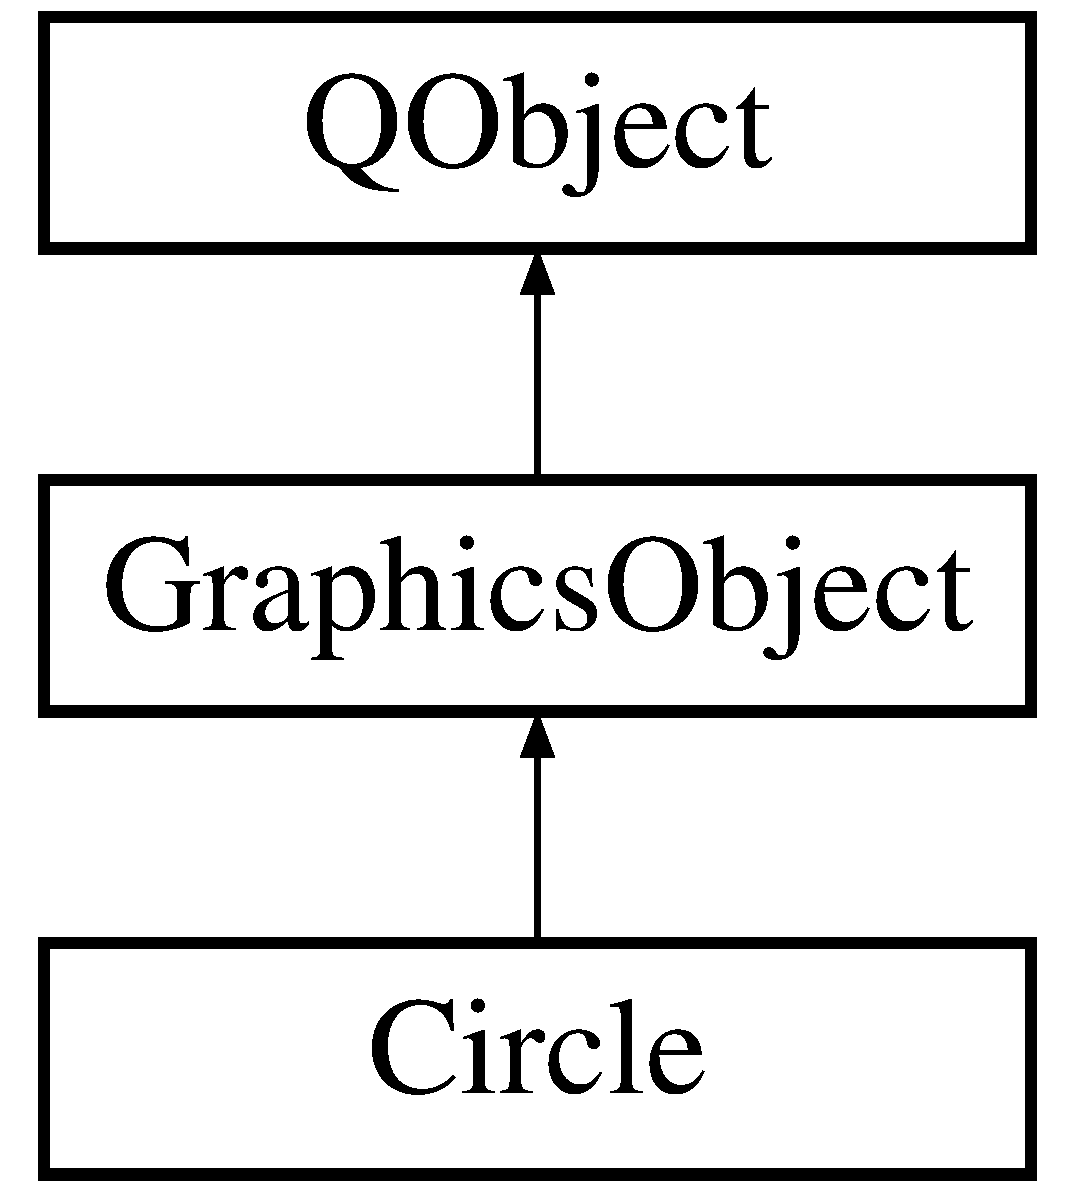
\includegraphics[height=3.000000cm]{class_circle}
\end{center}
\end{figure}
\subsection*{Public Member Functions}
\begin{DoxyCompactItemize}
\item 
\hyperlink{class_circle_a9851632042d96e4e534bebbec65e92c3}{Circle} (Q\+Object $\ast$parent=nullptr)
\begin{DoxyCompactList}\small\item\em \hyperlink{class_circle}{Circle} Kontruktor wid so geändert dass ein Q\+Object $\ast$parent -\/ Parameter erwartet wird. \end{DoxyCompactList}\item 
\hyperlink{class_circle_ae3f30436e645d73e368e8ee55f8d1650}{$\sim$\+Circle} ()
\begin{DoxyCompactList}\small\item\em \hyperlink{class_circle_ae3f30436e645d73e368e8ee55f8d1650}{Circle\+::$\sim$\+Circle} Dekonstruktor. \end{DoxyCompactList}\item 
\hyperlink{class_circle_a4e15e9f73da6961e60965dd2fdb0d19a}{Circle} (qreal xkoord, qreal ykoord, qreal width, qreal height, Q\+Color fill, Q\+Color border)
\begin{DoxyCompactList}\small\item\em \hyperlink{class_circle}{Circle}. \end{DoxyCompactList}\item 
virtual Q\+Abstract\+Graphics\+Shape\+Item $\ast$ \hyperlink{class_circle_a2c6dda8b50d9e19448d2e328b74430ce}{graphic\+Shape\+Item} () const
\begin{DoxyCompactList}\small\item\em graphic\+Shape\+Item \end{DoxyCompactList}\item 
virtual Q\+String \hyperlink{class_circle_a2fea55f4310daa23eb8c103bdcdcabd6}{to\+String} ()
\begin{DoxyCompactList}\small\item\em to\+String \end{DoxyCompactList}\end{DoxyCompactItemize}
\subsection*{Protected Attributes}
\begin{DoxyCompactItemize}
\item 
Q\+Graphics\+Ellipse\+Item $\ast$ \hyperlink{class_circle_aad3490d575b91461697136e1cad4e6a5}{m\+\_\+graphics\+Ellipse}
\end{DoxyCompactItemize}
\subsection*{Static Protected Attributes}
\begin{DoxyCompactItemize}
\item 
static unsigned long \hyperlink{class_circle_a0cd7c4ac1de2acb420970134f30075b2}{m\+\_\+circle\+Counter} = 0
\begin{DoxyCompactList}\small\item\em Initialisiert m\+\_\+circle\+Counter auf 0. \end{DoxyCompactList}\end{DoxyCompactItemize}


\subsection{Detailed Description}
The \hyperlink{class_circle}{Circle} class -\/ Kreis Klasse. 

\subsection{Constructor \& Destructor Documentation}
\mbox{\Hypertarget{class_circle_a9851632042d96e4e534bebbec65e92c3}\label{class_circle_a9851632042d96e4e534bebbec65e92c3}} 
\index{Circle@{Circle}!Circle@{Circle}}
\index{Circle@{Circle}!Circle@{Circle}}
\subsubsection{\texorpdfstring{Circle()}{Circle()}\hspace{0.1cm}{\footnotesize\ttfamily [1/2]}}
{\footnotesize\ttfamily Circle\+::\+Circle (\begin{DoxyParamCaption}\item[{Q\+Object $\ast$}]{parent = {\ttfamily nullptr} }\end{DoxyParamCaption})}



\hyperlink{class_circle}{Circle} Kontruktor wid so geändert dass ein Q\+Object $\ast$parent -\/ Parameter erwartet wird. 

\hyperlink{class_circle_a9851632042d96e4e534bebbec65e92c3}{Circle\+::\+Circle} Konstruktor.


\begin{DoxyParams}{Parameters}
{\em parent} & \\
\hline
\end{DoxyParams}
\mbox{\Hypertarget{class_circle_ae3f30436e645d73e368e8ee55f8d1650}\label{class_circle_ae3f30436e645d73e368e8ee55f8d1650}} 
\index{Circle@{Circle}!````~Circle@{$\sim$\+Circle}}
\index{````~Circle@{$\sim$\+Circle}!Circle@{Circle}}
\subsubsection{\texorpdfstring{$\sim$\+Circle()}{~Circle()}}
{\footnotesize\ttfamily Circle\+::$\sim$\+Circle (\begin{DoxyParamCaption}{ }\end{DoxyParamCaption})}



\hyperlink{class_circle_ae3f30436e645d73e368e8ee55f8d1650}{Circle\+::$\sim$\+Circle} Dekonstruktor. 

\mbox{\Hypertarget{class_circle_a4e15e9f73da6961e60965dd2fdb0d19a}\label{class_circle_a4e15e9f73da6961e60965dd2fdb0d19a}} 
\index{Circle@{Circle}!Circle@{Circle}}
\index{Circle@{Circle}!Circle@{Circle}}
\subsubsection{\texorpdfstring{Circle()}{Circle()}\hspace{0.1cm}{\footnotesize\ttfamily [2/2]}}
{\footnotesize\ttfamily Circle\+::\+Circle (\begin{DoxyParamCaption}\item[{qreal}]{xkoord,  }\item[{qreal}]{ykoord,  }\item[{qreal}]{width,  }\item[{qreal}]{height,  }\item[{Q\+Color}]{fill,  }\item[{Q\+Color}]{border }\end{DoxyParamCaption})}



\hyperlink{class_circle}{Circle}. 

\hyperlink{class_circle_a9851632042d96e4e534bebbec65e92c3}{Circle\+::\+Circle} Konstruktor, in dem ein Q\+Graphic\+Ellipse\+Item erstellt wird.


\begin{DoxyParams}{Parameters}
{\em xkoord} & \\
\hline
{\em ykoord} & \\
\hline
{\em width} & \\
\hline
{\em height} & \\
\hline
{\em fill} & \\
\hline
{\em border} & \\
\hline
\end{DoxyParams}


\subsection{Member Function Documentation}
\mbox{\Hypertarget{class_circle_a2c6dda8b50d9e19448d2e328b74430ce}\label{class_circle_a2c6dda8b50d9e19448d2e328b74430ce}} 
\index{Circle@{Circle}!graphic\+Shape\+Item@{graphic\+Shape\+Item}}
\index{graphic\+Shape\+Item@{graphic\+Shape\+Item}!Circle@{Circle}}
\subsubsection{\texorpdfstring{graphic\+Shape\+Item()}{graphicShapeItem()}}
{\footnotesize\ttfamily Q\+Abstract\+Graphics\+Shape\+Item $\ast$ Circle\+::graphic\+Shape\+Item (\begin{DoxyParamCaption}{ }\end{DoxyParamCaption}) const\hspace{0.3cm}{\ttfamily [virtual]}}



graphic\+Shape\+Item 

\hyperlink{class_circle_a2c6dda8b50d9e19448d2e328b74430ce}{Circle\+::graphic\+Shape\+Item}.

\begin{DoxyReturn}{Returns}


m\+\_\+graphics\+Ellipse 
\end{DoxyReturn}


Reimplemented from \hyperlink{class_graphics_object_ad898be2fdbcc4c57f908cdd6a3feaa44}{Graphics\+Object}.

\mbox{\Hypertarget{class_circle_a2fea55f4310daa23eb8c103bdcdcabd6}\label{class_circle_a2fea55f4310daa23eb8c103bdcdcabd6}} 
\index{Circle@{Circle}!to\+String@{to\+String}}
\index{to\+String@{to\+String}!Circle@{Circle}}
\subsubsection{\texorpdfstring{to\+String()}{toString()}}
{\footnotesize\ttfamily Q\+String Circle\+::to\+String (\begin{DoxyParamCaption}{ }\end{DoxyParamCaption})\hspace{0.3cm}{\ttfamily [virtual]}}



to\+String 

\hyperlink{class_circle_a2fea55f4310daa23eb8c103bdcdcabd6}{Circle\+::to\+String} gibt alle Daten des Q\+Graphic\+Object aus.

\begin{DoxyReturn}{Returns}

\end{DoxyReturn}


Reimplemented from \hyperlink{class_graphics_object_ad985316df1516a5a7311161250b5e233}{Graphics\+Object}.



\subsection{Member Data Documentation}
\mbox{\Hypertarget{class_circle_a0cd7c4ac1de2acb420970134f30075b2}\label{class_circle_a0cd7c4ac1de2acb420970134f30075b2}} 
\index{Circle@{Circle}!m\+\_\+circle\+Counter@{m\+\_\+circle\+Counter}}
\index{m\+\_\+circle\+Counter@{m\+\_\+circle\+Counter}!Circle@{Circle}}
\subsubsection{\texorpdfstring{m\+\_\+circle\+Counter}{m\_circleCounter}}
{\footnotesize\ttfamily unsigned long Circle\+::m\+\_\+circle\+Counter = 0\hspace{0.3cm}{\ttfamily [static]}, {\ttfamily [protected]}}



Initialisiert m\+\_\+circle\+Counter auf 0. 

\mbox{\Hypertarget{class_circle_aad3490d575b91461697136e1cad4e6a5}\label{class_circle_aad3490d575b91461697136e1cad4e6a5}} 
\index{Circle@{Circle}!m\+\_\+graphics\+Ellipse@{m\+\_\+graphics\+Ellipse}}
\index{m\+\_\+graphics\+Ellipse@{m\+\_\+graphics\+Ellipse}!Circle@{Circle}}
\subsubsection{\texorpdfstring{m\+\_\+graphics\+Ellipse}{m\_graphicsEllipse}}
{\footnotesize\ttfamily Q\+Graphics\+Ellipse\+Item$\ast$ Circle\+::m\+\_\+graphics\+Ellipse\hspace{0.3cm}{\ttfamily [protected]}}



The documentation for this class was generated from the following files\+:\begin{DoxyCompactItemize}
\item 
C\+:/\+Users/tranb/\+Desktop/\+Sciebo/\+Studium/\+Qt Projekte/\+Graphic\+Obj/\hyperlink{circle_8h}{circle.\+h}\item 
C\+:/\+Users/tranb/\+Desktop/\+Sciebo/\+Studium/\+Qt Projekte/\+Graphic\+Obj/\hyperlink{circle_8cpp}{circle.\+cpp}\end{DoxyCompactItemize}

\hypertarget{class_color_button}{}\section{Color\+Button Class Reference}
\label{class_color_button}\index{Color\+Button@{Color\+Button}}


The \hyperlink{class_color_button}{Color\+Button} class -\/ Klasse für die Farb Buttons abgeleitet von Q\+Push\+Button.  




{\ttfamily \#include $<$colorbutton.\+h$>$}

Inheritance diagram for Color\+Button\+:\begin{figure}[H]
\begin{center}
\leavevmode
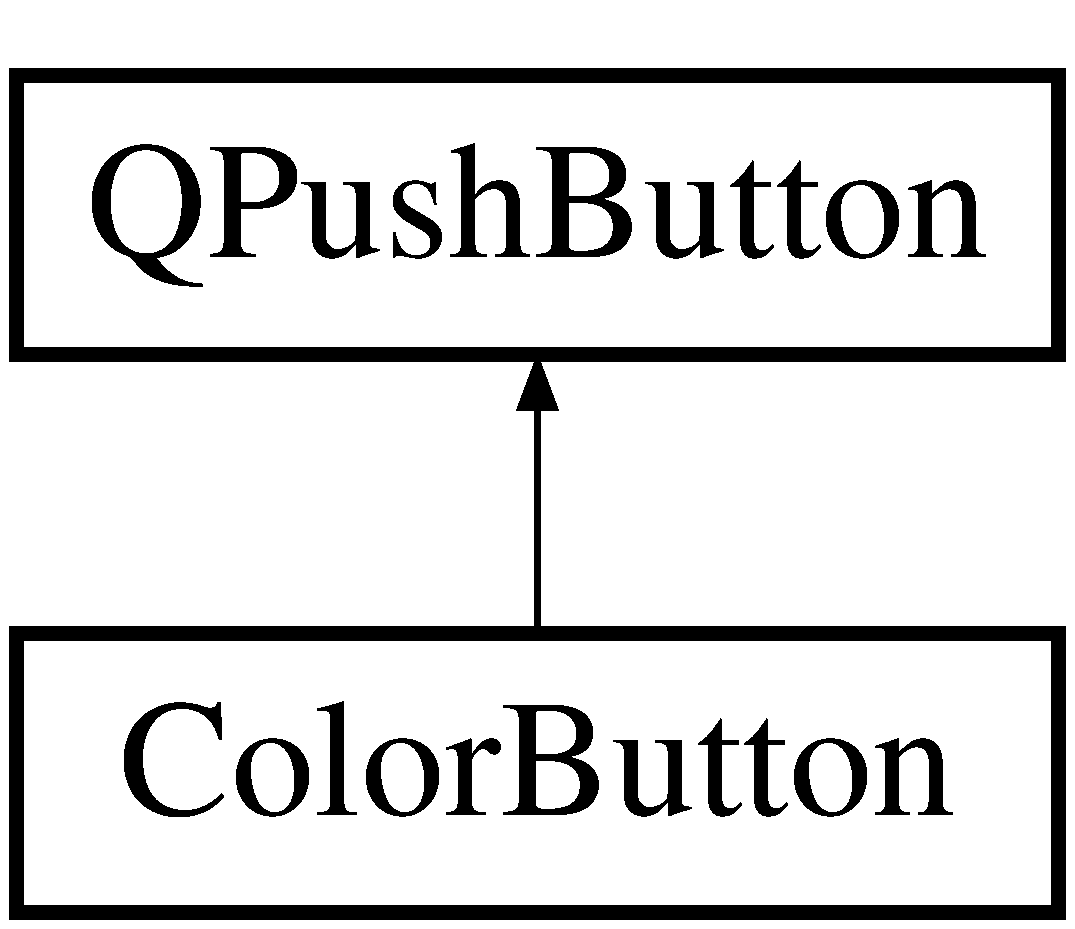
\includegraphics[height=2.000000cm]{class_color_button}
\end{center}
\end{figure}
\subsection*{Public Member Functions}
\begin{DoxyCompactItemize}
\item 
\hyperlink{class_color_button_a128b21900f22efdc9d71d0bffa0b64f8}{Color\+Button} (Q\+Widget $\ast$parent=0)
\begin{DoxyCompactList}\small\item\em \hyperlink{class_color_button_a128b21900f22efdc9d71d0bffa0b64f8}{Color\+Button\+::\+Color\+Button}. \end{DoxyCompactList}\item 
\hyperlink{class_color_button_a16f9cc31b3476fc5cb900e3692d4f49c}{Color\+Button} (Q\+Color \hyperlink{class_color_button_a7583a20c9a126ba93e344ea728c19954}{color}, Q\+Widget $\ast$parent=0)
\begin{DoxyCompactList}\small\item\em \hyperlink{class_color_button_a128b21900f22efdc9d71d0bffa0b64f8}{Color\+Button\+::\+Color\+Button}. \end{DoxyCompactList}\item 
void \hyperlink{class_color_button_ae7b2847c9974fb52f80d54dafc7a0f00}{paint\+Event} (Q\+Paint\+Event $\ast$)
\begin{DoxyCompactList}\small\item\em paint\+Event \end{DoxyCompactList}\item 
Q\+Color \hyperlink{class_color_button_a7583a20c9a126ba93e344ea728c19954}{color} () const
\begin{DoxyCompactList}\small\item\em Getter -\/ Methode für m\+\_\+color. \end{DoxyCompactList}\item 
void \hyperlink{class_color_button_ad0d3747c9ceb3ed57d3f513f42fd4cf2}{set\+Color} (const Q\+Color \&\hyperlink{class_color_button_a7583a20c9a126ba93e344ea728c19954}{color})
\begin{DoxyCompactList}\small\item\em Setter -\/ Methode für m\+\_\+color. \end{DoxyCompactList}\end{DoxyCompactItemize}
\subsection*{Protected Attributes}
\begin{DoxyCompactItemize}
\item 
Q\+Color \hyperlink{class_color_button_aa4408cd251575659e5e8417802f276e4}{m\+\_\+color}
\end{DoxyCompactItemize}


\subsection{Detailed Description}
The \hyperlink{class_color_button}{Color\+Button} class -\/ Klasse für die Farb Buttons abgeleitet von Q\+Push\+Button. 

\subsection{Constructor \& Destructor Documentation}
\mbox{\Hypertarget{class_color_button_a128b21900f22efdc9d71d0bffa0b64f8}\label{class_color_button_a128b21900f22efdc9d71d0bffa0b64f8}} 
\index{Color\+Button@{Color\+Button}!Color\+Button@{Color\+Button}}
\index{Color\+Button@{Color\+Button}!Color\+Button@{Color\+Button}}
\subsubsection{\texorpdfstring{Color\+Button()}{ColorButton()}\hspace{0.1cm}{\footnotesize\ttfamily [1/2]}}
{\footnotesize\ttfamily Color\+Button\+::\+Color\+Button (\begin{DoxyParamCaption}\item[{Q\+Widget $\ast$}]{parent = {\ttfamily 0} }\end{DoxyParamCaption})\hspace{0.3cm}{\ttfamily [explicit]}}



\hyperlink{class_color_button_a128b21900f22efdc9d71d0bffa0b64f8}{Color\+Button\+::\+Color\+Button}. 


\begin{DoxyParams}{Parameters}
{\em parent} & \\
\hline
\end{DoxyParams}
\mbox{\Hypertarget{class_color_button_a16f9cc31b3476fc5cb900e3692d4f49c}\label{class_color_button_a16f9cc31b3476fc5cb900e3692d4f49c}} 
\index{Color\+Button@{Color\+Button}!Color\+Button@{Color\+Button}}
\index{Color\+Button@{Color\+Button}!Color\+Button@{Color\+Button}}
\subsubsection{\texorpdfstring{Color\+Button()}{ColorButton()}\hspace{0.1cm}{\footnotesize\ttfamily [2/2]}}
{\footnotesize\ttfamily Color\+Button\+::\+Color\+Button (\begin{DoxyParamCaption}\item[{Q\+Color}]{color,  }\item[{Q\+Widget $\ast$}]{parent = {\ttfamily 0} }\end{DoxyParamCaption})\hspace{0.3cm}{\ttfamily [explicit]}}



\hyperlink{class_color_button_a128b21900f22efdc9d71d0bffa0b64f8}{Color\+Button\+::\+Color\+Button}. 


\begin{DoxyParams}{Parameters}
{\em color} & \\
\hline
{\em parent} & \\
\hline
\end{DoxyParams}


\subsection{Member Function Documentation}
\mbox{\Hypertarget{class_color_button_a7583a20c9a126ba93e344ea728c19954}\label{class_color_button_a7583a20c9a126ba93e344ea728c19954}} 
\index{Color\+Button@{Color\+Button}!color@{color}}
\index{color@{color}!Color\+Button@{Color\+Button}}
\subsubsection{\texorpdfstring{color()}{color()}}
{\footnotesize\ttfamily Q\+Color Color\+Button\+::color (\begin{DoxyParamCaption}{ }\end{DoxyParamCaption}) const}



Getter -\/ Methode für m\+\_\+color. 

\hyperlink{class_color_button_a7583a20c9a126ba93e344ea728c19954}{Color\+Button\+::color}.

\begin{DoxyReturn}{Returns}


m\+\_\+color 
\end{DoxyReturn}
\mbox{\Hypertarget{class_color_button_ae7b2847c9974fb52f80d54dafc7a0f00}\label{class_color_button_ae7b2847c9974fb52f80d54dafc7a0f00}} 
\index{Color\+Button@{Color\+Button}!paint\+Event@{paint\+Event}}
\index{paint\+Event@{paint\+Event}!Color\+Button@{Color\+Button}}
\subsubsection{\texorpdfstring{paint\+Event()}{paintEvent()}}
{\footnotesize\ttfamily void Color\+Button\+::paint\+Event (\begin{DoxyParamCaption}\item[{Q\+Paint\+Event $\ast$}]{paint }\end{DoxyParamCaption})}



paint\+Event 

\hyperlink{class_color_button_ae7b2847c9974fb52f80d54dafc7a0f00}{Color\+Button\+::paint\+Event}.


\begin{DoxyParams}{Parameters}
{\em paint} & \\
\hline
\end{DoxyParams}
Rechteck mit schwarzen Rahmen wird hier erstellt und bei der Breite und Höhe wird etwas abgezogen, damit das individuelle Rechteck kleiner ist als der Button x und y Werte werden auf 10 gesetzt damit das individuelle Rechteck Mittig liegt.

Individuelle Rechteck wird mit Farbe gefüllt und zwar mit der Farbe die vom Benutzer ausgewählt wid.\mbox{\Hypertarget{class_color_button_ad0d3747c9ceb3ed57d3f513f42fd4cf2}\label{class_color_button_ad0d3747c9ceb3ed57d3f513f42fd4cf2}} 
\index{Color\+Button@{Color\+Button}!set\+Color@{set\+Color}}
\index{set\+Color@{set\+Color}!Color\+Button@{Color\+Button}}
\subsubsection{\texorpdfstring{set\+Color()}{setColor()}}
{\footnotesize\ttfamily void Color\+Button\+::set\+Color (\begin{DoxyParamCaption}\item[{const Q\+Color \&}]{color }\end{DoxyParamCaption})}



Setter -\/ Methode für m\+\_\+color. 

\hyperlink{class_color_button_ad0d3747c9ceb3ed57d3f513f42fd4cf2}{Color\+Button\+::set\+Color}.


\begin{DoxyParams}{Parameters}
{\em color} & \\
\hline
\end{DoxyParams}


\subsection{Member Data Documentation}
\mbox{\Hypertarget{class_color_button_aa4408cd251575659e5e8417802f276e4}\label{class_color_button_aa4408cd251575659e5e8417802f276e4}} 
\index{Color\+Button@{Color\+Button}!m\+\_\+color@{m\+\_\+color}}
\index{m\+\_\+color@{m\+\_\+color}!Color\+Button@{Color\+Button}}
\subsubsection{\texorpdfstring{m\+\_\+color}{m\_color}}
{\footnotesize\ttfamily Q\+Color Color\+Button\+::m\+\_\+color\hspace{0.3cm}{\ttfamily [protected]}}



The documentation for this class was generated from the following files\+:\begin{DoxyCompactItemize}
\item 
C\+:/\+Users/tranb/\+Desktop/\+Sciebo/\+Studium/\+Qt Projekte/\+Graphic\+Obj/\hyperlink{colorbutton_8h}{colorbutton.\+h}\item 
C\+:/\+Users/tranb/\+Desktop/\+Sciebo/\+Studium/\+Qt Projekte/\+Graphic\+Obj/\hyperlink{colorbutton_8cpp}{colorbutton.\+cpp}\end{DoxyCompactItemize}

\hypertarget{class_color_selector}{}\section{Color\+Selector Class Reference}
\label{class_color_selector}\index{Color\+Selector@{Color\+Selector}}


The \hyperlink{class_color_selector}{Color\+Selector} class -\/ Eigenes Zusammengestelltes Widget für Farbwahl.  




{\ttfamily \#include $<$colorselector.\+h$>$}

Inheritance diagram for Color\+Selector\+:\begin{figure}[H]
\begin{center}
\leavevmode
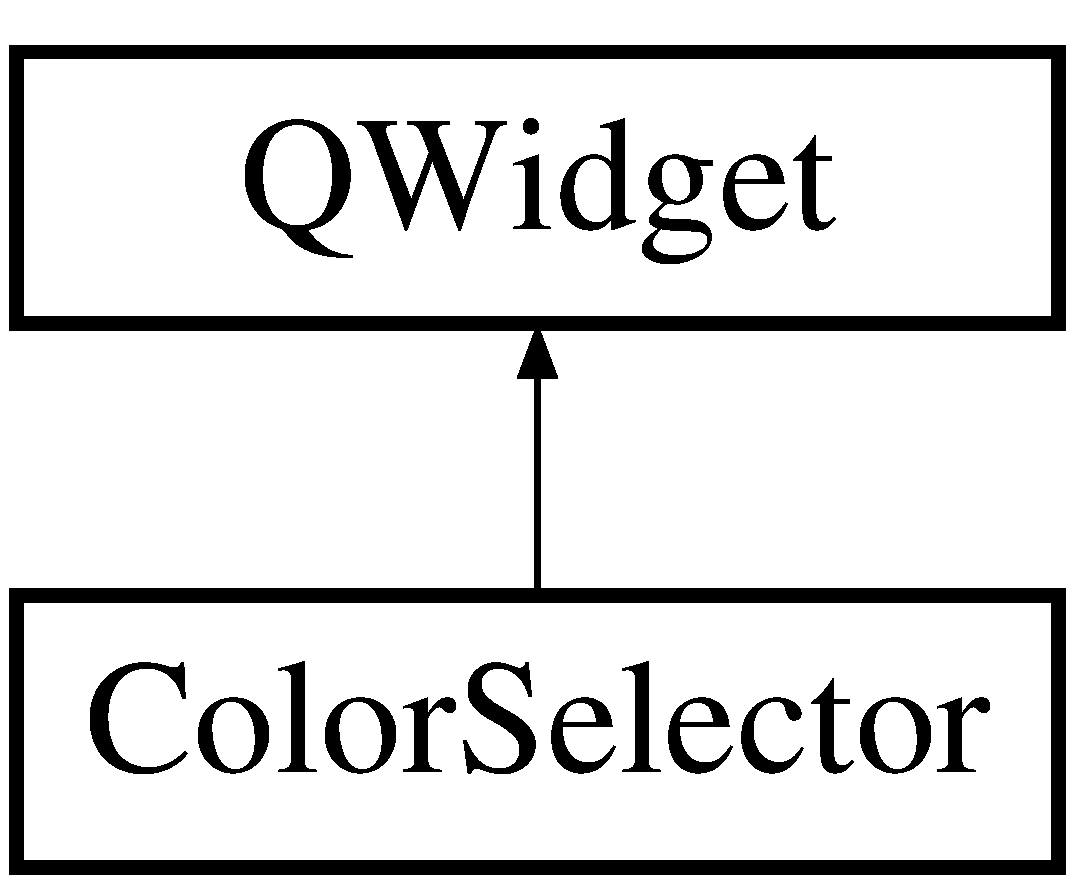
\includegraphics[height=2.000000cm]{class_color_selector}
\end{center}
\end{figure}
\subsection*{Signals}
\begin{DoxyCompactItemize}
\item 
void \hyperlink{class_color_selector_a3ba85a89666dd1ccb6e4274550e60e84}{active\+Border\+Color\+Changed} (Q\+Color color)
\begin{DoxyCompactList}\small\item\em active\+Border\+Color\+Changed -\/ Signal, um zu vermitteln, dass die Rahmenfarbe geändert wurde. \end{DoxyCompactList}\item 
void \hyperlink{class_color_selector_a62847504579be68c5bdb138ef7033b20}{active\+Fill\+Color\+Changed} (Q\+Color color)
\begin{DoxyCompactList}\small\item\em active\+Fill\+Color\+Changed -\/ Signal, um zu vermitteln, dass die Füllfarbe geändert wurde \end{DoxyCompactList}\end{DoxyCompactItemize}
\subsection*{Public Member Functions}
\begin{DoxyCompactItemize}
\item 
\hyperlink{class_color_selector_aa8669eb9e5da7ca151ef84fba84a5f34}{Color\+Selector} (Q\+Widget $\ast$parent=0)
\begin{DoxyCompactList}\small\item\em \hyperlink{class_color_selector_aa8669eb9e5da7ca151ef84fba84a5f34}{Color\+Selector\+::\+Color\+Selector}. \end{DoxyCompactList}\item 
\hyperlink{class_color_selector_a8c5de1d7bf1515c11ba0157e2b11aff4}{$\sim$\+Color\+Selector} ()
\begin{DoxyCompactList}\small\item\em \hyperlink{class_color_selector_a8c5de1d7bf1515c11ba0157e2b11aff4}{Color\+Selector\+::$\sim$\+Color\+Selector}. \end{DoxyCompactList}\end{DoxyCompactItemize}


\subsection{Detailed Description}
The \hyperlink{class_color_selector}{Color\+Selector} class -\/ Eigenes Zusammengestelltes Widget für Farbwahl. 

\subsection{Constructor \& Destructor Documentation}
\mbox{\Hypertarget{class_color_selector_aa8669eb9e5da7ca151ef84fba84a5f34}\label{class_color_selector_aa8669eb9e5da7ca151ef84fba84a5f34}} 
\index{Color\+Selector@{Color\+Selector}!Color\+Selector@{Color\+Selector}}
\index{Color\+Selector@{Color\+Selector}!Color\+Selector@{Color\+Selector}}
\subsubsection{\texorpdfstring{Color\+Selector()}{ColorSelector()}}
{\footnotesize\ttfamily Color\+Selector\+::\+Color\+Selector (\begin{DoxyParamCaption}\item[{Q\+Widget $\ast$}]{parent = {\ttfamily 0} }\end{DoxyParamCaption})\hspace{0.3cm}{\ttfamily [explicit]}}



\hyperlink{class_color_selector_aa8669eb9e5da7ca151ef84fba84a5f34}{Color\+Selector\+::\+Color\+Selector}. 


\begin{DoxyParams}{Parameters}
{\em parent} & \\
\hline
\end{DoxyParams}
\mbox{\Hypertarget{class_color_selector_a8c5de1d7bf1515c11ba0157e2b11aff4}\label{class_color_selector_a8c5de1d7bf1515c11ba0157e2b11aff4}} 
\index{Color\+Selector@{Color\+Selector}!````~Color\+Selector@{$\sim$\+Color\+Selector}}
\index{````~Color\+Selector@{$\sim$\+Color\+Selector}!Color\+Selector@{Color\+Selector}}
\subsubsection{\texorpdfstring{$\sim$\+Color\+Selector()}{~ColorSelector()}}
{\footnotesize\ttfamily Color\+Selector\+::$\sim$\+Color\+Selector (\begin{DoxyParamCaption}{ }\end{DoxyParamCaption})}



\hyperlink{class_color_selector_a8c5de1d7bf1515c11ba0157e2b11aff4}{Color\+Selector\+::$\sim$\+Color\+Selector}. 



\subsection{Member Function Documentation}
\mbox{\Hypertarget{class_color_selector_a3ba85a89666dd1ccb6e4274550e60e84}\label{class_color_selector_a3ba85a89666dd1ccb6e4274550e60e84}} 
\index{Color\+Selector@{Color\+Selector}!active\+Border\+Color\+Changed@{active\+Border\+Color\+Changed}}
\index{active\+Border\+Color\+Changed@{active\+Border\+Color\+Changed}!Color\+Selector@{Color\+Selector}}
\subsubsection{\texorpdfstring{active\+Border\+Color\+Changed}{activeBorderColorChanged}}
{\footnotesize\ttfamily void Color\+Selector\+::active\+Border\+Color\+Changed (\begin{DoxyParamCaption}\item[{Q\+Color}]{color }\end{DoxyParamCaption})\hspace{0.3cm}{\ttfamily [signal]}}



active\+Border\+Color\+Changed -\/ Signal, um zu vermitteln, dass die Rahmenfarbe geändert wurde. 


\begin{DoxyParams}{Parameters}
{\em color} & \\
\hline
\end{DoxyParams}
\mbox{\Hypertarget{class_color_selector_a62847504579be68c5bdb138ef7033b20}\label{class_color_selector_a62847504579be68c5bdb138ef7033b20}} 
\index{Color\+Selector@{Color\+Selector}!active\+Fill\+Color\+Changed@{active\+Fill\+Color\+Changed}}
\index{active\+Fill\+Color\+Changed@{active\+Fill\+Color\+Changed}!Color\+Selector@{Color\+Selector}}
\subsubsection{\texorpdfstring{active\+Fill\+Color\+Changed}{activeFillColorChanged}}
{\footnotesize\ttfamily void Color\+Selector\+::active\+Fill\+Color\+Changed (\begin{DoxyParamCaption}\item[{Q\+Color}]{color }\end{DoxyParamCaption})\hspace{0.3cm}{\ttfamily [signal]}}



active\+Fill\+Color\+Changed -\/ Signal, um zu vermitteln, dass die Füllfarbe geändert wurde 


\begin{DoxyParams}{Parameters}
{\em color} & \\
\hline
\end{DoxyParams}


The documentation for this class was generated from the following files\+:\begin{DoxyCompactItemize}
\item 
C\+:/\+Users/tranb/\+Desktop/\+Sciebo/\+Studium/\+Qt Projekte/\+Graphic\+Obj/\hyperlink{colorselector_8h}{colorselector.\+h}\item 
C\+:/\+Users/tranb/\+Desktop/\+Sciebo/\+Studium/\+Qt Projekte/\+Graphic\+Obj/\hyperlink{colorselector_8cpp}{colorselector.\+cpp}\end{DoxyCompactItemize}

\hypertarget{class_drawing_tool_selector}{}\section{Drawing\+Tool\+Selector Class Reference}
\label{class_drawing_tool_selector}\index{Drawing\+Tool\+Selector@{Drawing\+Tool\+Selector}}


The \hyperlink{class_drawing_tool_selector}{Drawing\+Tool\+Selector} class -\/ Eigenes zusammengestelltes Widget für die Auswahl an Zeichenoptionen.  




{\ttfamily \#include $<$drawingtoolselector.\+h$>$}

Inheritance diagram for Drawing\+Tool\+Selector\+:\begin{figure}[H]
\begin{center}
\leavevmode
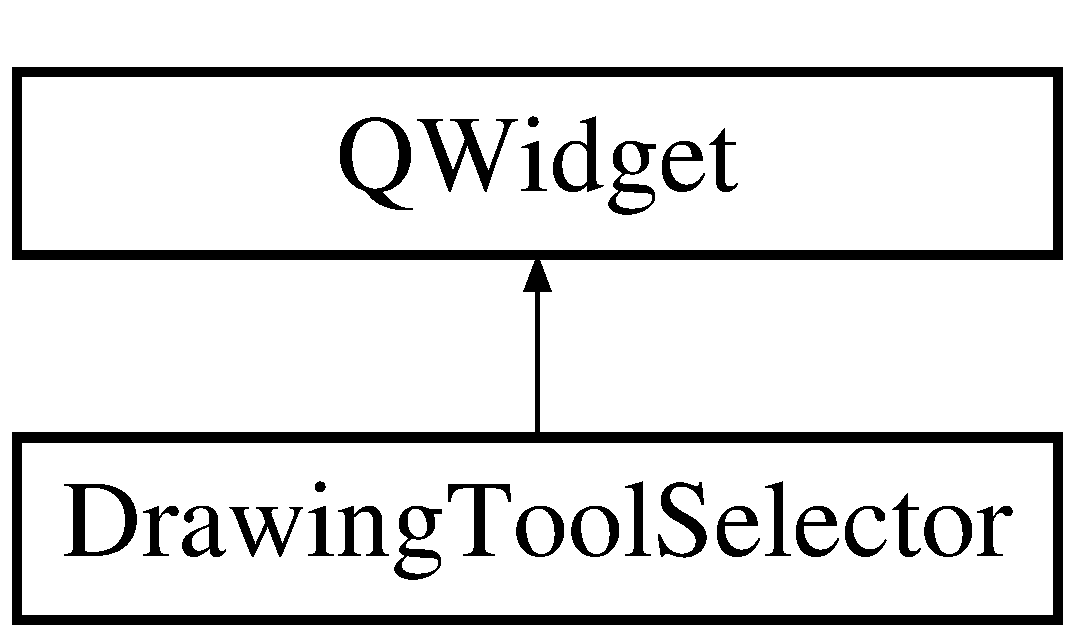
\includegraphics[height=2.000000cm]{class_drawing_tool_selector}
\end{center}
\end{figure}
\subsection*{Signals}
\begin{DoxyCompactItemize}
\item 
void \hyperlink{class_drawing_tool_selector_afd6c053c93d273fc110e8f11c0631ff3}{active\+Drawing\+Tool\+Changed} (\hyperlink{class_tools_ab031688a77e89a80ce8b5db7014684a3}{Tools\+::\+Draw\+Tool} active\+Drawing\+Tool)
\begin{DoxyCompactList}\small\item\em active\+Drawing\+Tool\+Changed -\/ Signal um zu vemitteln, dass das Zeichenwerkzeug geändert wurde. \end{DoxyCompactList}\item 
void \hyperlink{class_drawing_tool_selector_a062791d4a8183a6f20ecd12975ddc72d}{active\+Option\+Tool\+Changed} (\hyperlink{class_tools_a4b55b2ca4eef4d80ae1042233832bb8b}{Tools\+::\+Option\+Tool} active\+Option\+Tool)
\begin{DoxyCompactList}\small\item\em active\+Option\+Tool\+Changed \end{DoxyCompactList}\end{DoxyCompactItemize}
\subsection*{Public Member Functions}
\begin{DoxyCompactItemize}
\item 
\hyperlink{class_drawing_tool_selector_a04f21c51c1c8eefe90c7974d1551ba7e}{Drawing\+Tool\+Selector} (Q\+Widget $\ast$parent=0)
\item 
\hyperlink{class_drawing_tool_selector_ad5f2e810c40bbeb995711860f6a22394}{$\sim$\+Drawing\+Tool\+Selector} ()
\begin{DoxyCompactList}\small\item\em \hyperlink{class_drawing_tool_selector_ad5f2e810c40bbeb995711860f6a22394}{Drawing\+Tool\+Selector\+::$\sim$\+Drawing\+Tool\+Selector}. \end{DoxyCompactList}\end{DoxyCompactItemize}


\subsection{Detailed Description}
The \hyperlink{class_drawing_tool_selector}{Drawing\+Tool\+Selector} class -\/ Eigenes zusammengestelltes Widget für die Auswahl an Zeichenoptionen. 

\subsection{Constructor \& Destructor Documentation}
\mbox{\Hypertarget{class_drawing_tool_selector_a04f21c51c1c8eefe90c7974d1551ba7e}\label{class_drawing_tool_selector_a04f21c51c1c8eefe90c7974d1551ba7e}} 
\index{Drawing\+Tool\+Selector@{Drawing\+Tool\+Selector}!Drawing\+Tool\+Selector@{Drawing\+Tool\+Selector}}
\index{Drawing\+Tool\+Selector@{Drawing\+Tool\+Selector}!Drawing\+Tool\+Selector@{Drawing\+Tool\+Selector}}
\subsubsection{\texorpdfstring{Drawing\+Tool\+Selector()}{DrawingToolSelector()}}
{\footnotesize\ttfamily Drawing\+Tool\+Selector\+::\+Drawing\+Tool\+Selector (\begin{DoxyParamCaption}\item[{Q\+Widget $\ast$}]{parent = {\ttfamily 0} }\end{DoxyParamCaption})\hspace{0.3cm}{\ttfamily [explicit]}}

$<$ Default Set\+Up für m\+\_\+active\+Drawing\+Tool

$<$Default Set\+Up für m\+\_\+active\+Option\+Tool \mbox{\Hypertarget{class_drawing_tool_selector_ad5f2e810c40bbeb995711860f6a22394}\label{class_drawing_tool_selector_ad5f2e810c40bbeb995711860f6a22394}} 
\index{Drawing\+Tool\+Selector@{Drawing\+Tool\+Selector}!````~Drawing\+Tool\+Selector@{$\sim$\+Drawing\+Tool\+Selector}}
\index{````~Drawing\+Tool\+Selector@{$\sim$\+Drawing\+Tool\+Selector}!Drawing\+Tool\+Selector@{Drawing\+Tool\+Selector}}
\subsubsection{\texorpdfstring{$\sim$\+Drawing\+Tool\+Selector()}{~DrawingToolSelector()}}
{\footnotesize\ttfamily Drawing\+Tool\+Selector\+::$\sim$\+Drawing\+Tool\+Selector (\begin{DoxyParamCaption}{ }\end{DoxyParamCaption})}



\hyperlink{class_drawing_tool_selector_ad5f2e810c40bbeb995711860f6a22394}{Drawing\+Tool\+Selector\+::$\sim$\+Drawing\+Tool\+Selector}. 



\subsection{Member Function Documentation}
\mbox{\Hypertarget{class_drawing_tool_selector_afd6c053c93d273fc110e8f11c0631ff3}\label{class_drawing_tool_selector_afd6c053c93d273fc110e8f11c0631ff3}} 
\index{Drawing\+Tool\+Selector@{Drawing\+Tool\+Selector}!active\+Drawing\+Tool\+Changed@{active\+Drawing\+Tool\+Changed}}
\index{active\+Drawing\+Tool\+Changed@{active\+Drawing\+Tool\+Changed}!Drawing\+Tool\+Selector@{Drawing\+Tool\+Selector}}
\subsubsection{\texorpdfstring{active\+Drawing\+Tool\+Changed}{activeDrawingToolChanged}}
{\footnotesize\ttfamily void Drawing\+Tool\+Selector\+::active\+Drawing\+Tool\+Changed (\begin{DoxyParamCaption}\item[{\hyperlink{class_tools_ab031688a77e89a80ce8b5db7014684a3}{Tools\+::\+Draw\+Tool}}]{active\+Drawing\+Tool }\end{DoxyParamCaption})\hspace{0.3cm}{\ttfamily [signal]}}



active\+Drawing\+Tool\+Changed -\/ Signal um zu vemitteln, dass das Zeichenwerkzeug geändert wurde. 


\begin{DoxyParams}{Parameters}
{\em active\+Drawing\+Tool} & \\
\hline
\end{DoxyParams}
\mbox{\Hypertarget{class_drawing_tool_selector_a062791d4a8183a6f20ecd12975ddc72d}\label{class_drawing_tool_selector_a062791d4a8183a6f20ecd12975ddc72d}} 
\index{Drawing\+Tool\+Selector@{Drawing\+Tool\+Selector}!active\+Option\+Tool\+Changed@{active\+Option\+Tool\+Changed}}
\index{active\+Option\+Tool\+Changed@{active\+Option\+Tool\+Changed}!Drawing\+Tool\+Selector@{Drawing\+Tool\+Selector}}
\subsubsection{\texorpdfstring{active\+Option\+Tool\+Changed}{activeOptionToolChanged}}
{\footnotesize\ttfamily void Drawing\+Tool\+Selector\+::active\+Option\+Tool\+Changed (\begin{DoxyParamCaption}\item[{\hyperlink{class_tools_a4b55b2ca4eef4d80ae1042233832bb8b}{Tools\+::\+Option\+Tool}}]{active\+Option\+Tool }\end{DoxyParamCaption})\hspace{0.3cm}{\ttfamily [signal]}}



active\+Option\+Tool\+Changed 


\begin{DoxyParams}{Parameters}
{\em active\+Option\+Tool} & \\
\hline
\end{DoxyParams}


The documentation for this class was generated from the following files\+:\begin{DoxyCompactItemize}
\item 
C\+:/\+Users/tranb/\+Desktop/\+Sciebo/\+Studium/\+Qt Projekte/\+Graphic\+Obj/\hyperlink{drawingtoolselector_8h}{drawingtoolselector.\+h}\item 
C\+:/\+Users/tranb/\+Desktop/\+Sciebo/\+Studium/\+Qt Projekte/\+Graphic\+Obj/\hyperlink{drawingtoolselector_8cpp}{drawingtoolselector.\+cpp}\end{DoxyCompactItemize}

\hypertarget{class_graphics_object}{}\section{Graphics\+Object Class Reference}
\label{class_graphics_object}\index{Graphics\+Object@{Graphics\+Object}}


The \hyperlink{class_graphics_object}{Graphics\+Object} class -\/ Klass für das Grafik Objekt abgeleitet von Q\+Object.  




{\ttfamily \#include $<$graphicsobject.\+h$>$}

Inheritance diagram for Graphics\+Object\+:\begin{figure}[H]
\begin{center}
\leavevmode
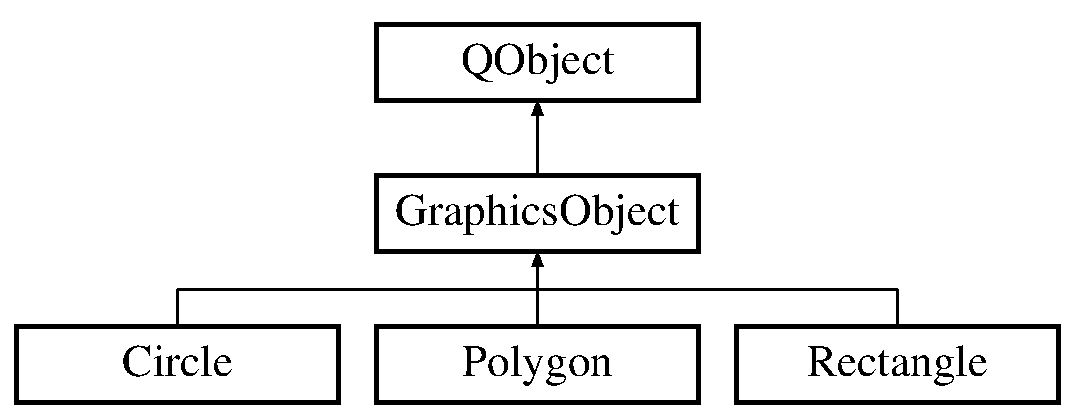
\includegraphics[height=3.000000cm]{class_graphics_object}
\end{center}
\end{figure}
\subsection*{Public Member Functions}
\begin{DoxyCompactItemize}
\item 
\hyperlink{class_graphics_object_a82fb630ff536190739e347b68716f603}{Graphics\+Object} (Q\+Object $\ast$parent=nullptr)
\begin{DoxyCompactList}\small\item\em \hyperlink{class_graphics_object_a82fb630ff536190739e347b68716f603}{Graphics\+Object\+::\+Graphics\+Object}. \end{DoxyCompactList}\item 
Q\+String \hyperlink{class_graphics_object_ac5591ff2b8009451c593d1197ce7a162}{name} () const
\begin{DoxyCompactList}\small\item\em Getter -\/ Methode für name. \end{DoxyCompactList}\item 
void \hyperlink{class_graphics_object_a1b0c7c7f87e86833a9a23ab1a2b6f685}{set\+Name} (const Q\+String \&\hyperlink{class_graphics_object_ac5591ff2b8009451c593d1197ce7a162}{name})
\begin{DoxyCompactList}\small\item\em set\+Name -\/ Methode \end{DoxyCompactList}\item 
virtual Q\+Abstract\+Graphics\+Shape\+Item $\ast$ \hyperlink{class_graphics_object_ad898be2fdbcc4c57f908cdd6a3feaa44}{graphic\+Shape\+Item} () const
\begin{DoxyCompactList}\small\item\em graphic\+Shape\+Item \end{DoxyCompactList}\item 
virtual Q\+String \hyperlink{class_graphics_object_ad985316df1516a5a7311161250b5e233}{to\+String} ()
\begin{DoxyCompactList}\small\item\em to\+String \end{DoxyCompactList}\end{DoxyCompactItemize}
\subsection*{Protected Attributes}
\begin{DoxyCompactItemize}
\item 
Q\+String \hyperlink{class_graphics_object_aaa6fae9a6fac8fd912b3bf5b3c98fc26}{m\+\_\+name}
\end{DoxyCompactItemize}
\subsection*{Static Protected Attributes}
\begin{DoxyCompactItemize}
\item 
static unsigned long \hyperlink{class_graphics_object_a09b02b61e4f9c5aefed46c3625cb98ed}{m\+\_\+graphics\+Object\+Counter} = 0
\begin{DoxyCompactList}\small\item\em Graphics\+Object\+Counter wird initialisiert. \end{DoxyCompactList}\end{DoxyCompactItemize}


\subsection{Detailed Description}
The \hyperlink{class_graphics_object}{Graphics\+Object} class -\/ Klass für das Grafik Objekt abgeleitet von Q\+Object. 

\subsection{Constructor \& Destructor Documentation}
\mbox{\Hypertarget{class_graphics_object_a82fb630ff536190739e347b68716f603}\label{class_graphics_object_a82fb630ff536190739e347b68716f603}} 
\index{Graphics\+Object@{Graphics\+Object}!Graphics\+Object@{Graphics\+Object}}
\index{Graphics\+Object@{Graphics\+Object}!Graphics\+Object@{Graphics\+Object}}
\subsubsection{\texorpdfstring{Graphics\+Object()}{GraphicsObject()}}
{\footnotesize\ttfamily Graphics\+Object\+::\+Graphics\+Object (\begin{DoxyParamCaption}\item[{Q\+Object $\ast$}]{parent = {\ttfamily nullptr} }\end{DoxyParamCaption})\hspace{0.3cm}{\ttfamily [explicit]}}



\hyperlink{class_graphics_object_a82fb630ff536190739e347b68716f603}{Graphics\+Object\+::\+Graphics\+Object}. 


\begin{DoxyParams}{Parameters}
{\em parent} & \\
\hline
\end{DoxyParams}


\subsection{Member Function Documentation}
\mbox{\Hypertarget{class_graphics_object_ad898be2fdbcc4c57f908cdd6a3feaa44}\label{class_graphics_object_ad898be2fdbcc4c57f908cdd6a3feaa44}} 
\index{Graphics\+Object@{Graphics\+Object}!graphic\+Shape\+Item@{graphic\+Shape\+Item}}
\index{graphic\+Shape\+Item@{graphic\+Shape\+Item}!Graphics\+Object@{Graphics\+Object}}
\subsubsection{\texorpdfstring{graphic\+Shape\+Item()}{graphicShapeItem()}}
{\footnotesize\ttfamily Q\+Abstract\+Graphics\+Shape\+Item $\ast$ Graphics\+Object\+::graphic\+Shape\+Item (\begin{DoxyParamCaption}{ }\end{DoxyParamCaption}) const\hspace{0.3cm}{\ttfamily [virtual]}}



graphic\+Shape\+Item 

\hyperlink{class_graphics_object_ad898be2fdbcc4c57f908cdd6a3feaa44}{Graphics\+Object\+::graphic\+Shape\+Item}.

\begin{DoxyReturn}{Returns}


0 
\end{DoxyReturn}


Reimplemented in \hyperlink{class_polygon_aebf0f177dbc4da17a1822be5a0063b25}{Polygon}, \hyperlink{class_rectangle_aeafbe16d72e37bb155c78a122408d3dc}{Rectangle}, and \hyperlink{class_circle_a2c6dda8b50d9e19448d2e328b74430ce}{Circle}.

\mbox{\Hypertarget{class_graphics_object_ac5591ff2b8009451c593d1197ce7a162}\label{class_graphics_object_ac5591ff2b8009451c593d1197ce7a162}} 
\index{Graphics\+Object@{Graphics\+Object}!name@{name}}
\index{name@{name}!Graphics\+Object@{Graphics\+Object}}
\subsubsection{\texorpdfstring{name()}{name()}}
{\footnotesize\ttfamily Q\+String Graphics\+Object\+::name (\begin{DoxyParamCaption}{ }\end{DoxyParamCaption}) const}



Getter -\/ Methode für name. 

Getter -\/ Methode für den Namen des \hyperlink{class_graphics_object}{Graphics\+Object} -\/ Objekt.

\begin{DoxyReturn}{Returns}
m\+\_\+name 
\end{DoxyReturn}
\mbox{\Hypertarget{class_graphics_object_a1b0c7c7f87e86833a9a23ab1a2b6f685}\label{class_graphics_object_a1b0c7c7f87e86833a9a23ab1a2b6f685}} 
\index{Graphics\+Object@{Graphics\+Object}!set\+Name@{set\+Name}}
\index{set\+Name@{set\+Name}!Graphics\+Object@{Graphics\+Object}}
\subsubsection{\texorpdfstring{set\+Name()}{setName()}}
{\footnotesize\ttfamily void Graphics\+Object\+::set\+Name (\begin{DoxyParamCaption}\item[{const Q\+String \&}]{name }\end{DoxyParamCaption})}



set\+Name -\/ Methode 

Setter -\/ Methode für Name des \hyperlink{class_graphics_object}{Graphics\+Object} -\/ Objekt.


\begin{DoxyParams}{Parameters}
{\em name} & \\
\hline
\end{DoxyParams}
$<$to\+Utf8 gibt die Q\+String werte als Schrift aus. \mbox{\Hypertarget{class_graphics_object_ad985316df1516a5a7311161250b5e233}\label{class_graphics_object_ad985316df1516a5a7311161250b5e233}} 
\index{Graphics\+Object@{Graphics\+Object}!to\+String@{to\+String}}
\index{to\+String@{to\+String}!Graphics\+Object@{Graphics\+Object}}
\subsubsection{\texorpdfstring{to\+String()}{toString()}}
{\footnotesize\ttfamily Q\+String Graphics\+Object\+::to\+String (\begin{DoxyParamCaption}{ }\end{DoxyParamCaption})\hspace{0.3cm}{\ttfamily [virtual]}}



to\+String 

\hyperlink{class_graphics_object_ad985316df1516a5a7311161250b5e233}{Graphics\+Object\+::to\+String}.

\begin{DoxyReturn}{Returns}


m\+\_\+name. 
\end{DoxyReturn}


Reimplemented in \hyperlink{class_polygon_a588df36c92bfa626e0a16acb07162fa3}{Polygon}, \hyperlink{class_rectangle_a75b1e77ef828ff8de86cfcf6b03bfadb}{Rectangle}, and \hyperlink{class_circle_a2fea55f4310daa23eb8c103bdcdcabd6}{Circle}.



\subsection{Member Data Documentation}
\mbox{\Hypertarget{class_graphics_object_a09b02b61e4f9c5aefed46c3625cb98ed}\label{class_graphics_object_a09b02b61e4f9c5aefed46c3625cb98ed}} 
\index{Graphics\+Object@{Graphics\+Object}!m\+\_\+graphics\+Object\+Counter@{m\+\_\+graphics\+Object\+Counter}}
\index{m\+\_\+graphics\+Object\+Counter@{m\+\_\+graphics\+Object\+Counter}!Graphics\+Object@{Graphics\+Object}}
\subsubsection{\texorpdfstring{m\+\_\+graphics\+Object\+Counter}{m\_graphicsObjectCounter}}
{\footnotesize\ttfamily unsigned long Graphics\+Object\+::m\+\_\+graphics\+Object\+Counter = 0\hspace{0.3cm}{\ttfamily [static]}, {\ttfamily [protected]}}



Graphics\+Object\+Counter wird initialisiert. 

\mbox{\Hypertarget{class_graphics_object_aaa6fae9a6fac8fd912b3bf5b3c98fc26}\label{class_graphics_object_aaa6fae9a6fac8fd912b3bf5b3c98fc26}} 
\index{Graphics\+Object@{Graphics\+Object}!m\+\_\+name@{m\+\_\+name}}
\index{m\+\_\+name@{m\+\_\+name}!Graphics\+Object@{Graphics\+Object}}
\subsubsection{\texorpdfstring{m\+\_\+name}{m\_name}}
{\footnotesize\ttfamily Q\+String Graphics\+Object\+::m\+\_\+name\hspace{0.3cm}{\ttfamily [protected]}}



The documentation for this class was generated from the following files\+:\begin{DoxyCompactItemize}
\item 
C\+:/\+Users/tranb/\+Desktop/\+Sciebo/\+Studium/\+Qt Projekte/\+Graphic\+Obj/\hyperlink{graphicsobject_8h}{graphicsobject.\+h}\item 
C\+:/\+Users/tranb/\+Desktop/\+Sciebo/\+Studium/\+Qt Projekte/\+Graphic\+Obj/\hyperlink{graphicsobject_8cpp}{graphicsobject.\+cpp}\end{DoxyCompactItemize}

\hypertarget{class_graphics_objects_map}{}\section{Graphics\+Objects\+Map Class Reference}
\label{class_graphics_objects_map}\index{Graphics\+Objects\+Map@{Graphics\+Objects\+Map}}


The \hyperlink{class_graphics_objects_map}{Graphics\+Objects\+Map} class -\/ Klasse für die \hyperlink{class_graphics_objects_map}{Graphics\+Objects\+Map}.  




{\ttfamily \#include $<$graphicsobjectsmap.\+h$>$}

Inheritance diagram for Graphics\+Objects\+Map\+:\begin{figure}[H]
\begin{center}
\leavevmode
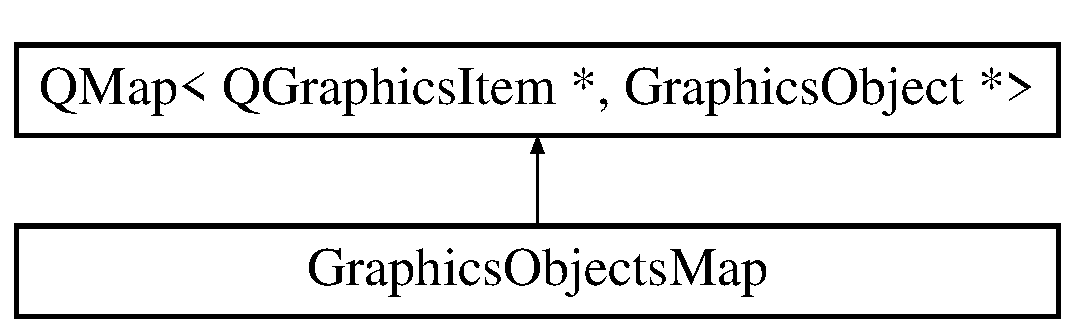
\includegraphics[height=2.000000cm]{class_graphics_objects_map}
\end{center}
\end{figure}
\subsection*{Public Member Functions}
\begin{DoxyCompactItemize}
\item 
\hyperlink{class_graphics_objects_map_a15a79dc2d1a2ab517cf5c5ccce3f05bc}{Graphics\+Objects\+Map} ()
\begin{DoxyCompactList}\small\item\em \hyperlink{class_graphics_objects_map}{Graphics\+Objects\+Map}. \end{DoxyCompactList}\end{DoxyCompactItemize}


\subsection{Detailed Description}
The \hyperlink{class_graphics_objects_map}{Graphics\+Objects\+Map} class -\/ Klasse für die \hyperlink{class_graphics_objects_map}{Graphics\+Objects\+Map}. 

\subsection{Constructor \& Destructor Documentation}
\mbox{\Hypertarget{class_graphics_objects_map_a15a79dc2d1a2ab517cf5c5ccce3f05bc}\label{class_graphics_objects_map_a15a79dc2d1a2ab517cf5c5ccce3f05bc}} 
\index{Graphics\+Objects\+Map@{Graphics\+Objects\+Map}!Graphics\+Objects\+Map@{Graphics\+Objects\+Map}}
\index{Graphics\+Objects\+Map@{Graphics\+Objects\+Map}!Graphics\+Objects\+Map@{Graphics\+Objects\+Map}}
\subsubsection{\texorpdfstring{Graphics\+Objects\+Map()}{GraphicsObjectsMap()}}
{\footnotesize\ttfamily Graphics\+Objects\+Map\+::\+Graphics\+Objects\+Map (\begin{DoxyParamCaption}{ }\end{DoxyParamCaption})}



\hyperlink{class_graphics_objects_map}{Graphics\+Objects\+Map}. 

\hyperlink{class_graphics_objects_map_a15a79dc2d1a2ab517cf5c5ccce3f05bc}{Graphics\+Objects\+Map\+::\+Graphics\+Objects\+Map}. Liste in der die Objekte gespeichert werden. 

The documentation for this class was generated from the following files\+:\begin{DoxyCompactItemize}
\item 
C\+:/\+Users/tranb/\+Desktop/\+Sciebo/\+Studium/\+Qt Projekte/\+Graphic\+Obj/\hyperlink{graphicsobjectsmap_8h}{graphicsobjectsmap.\+h}\item 
C\+:/\+Users/tranb/\+Desktop/\+Sciebo/\+Studium/\+Qt Projekte/\+Graphic\+Obj/\hyperlink{graphicsobjectsmap_8cpp}{graphicsobjectsmap.\+cpp}\end{DoxyCompactItemize}

\hypertarget{class_graphics_scene}{}\section{Graphics\+Scene Class Reference}
\label{class_graphics_scene}\index{Graphics\+Scene@{Graphics\+Scene}}


The \hyperlink{class_graphics_scene}{Graphics\+Scene} class -\/ Klasse für die \hyperlink{class_graphics_scene}{Graphics\+Scene} abgeleitet von Q\+Graphics\+Scene.  




{\ttfamily \#include $<$graphicsscene.\+h$>$}

Inheritance diagram for Graphics\+Scene\+:\begin{figure}[H]
\begin{center}
\leavevmode
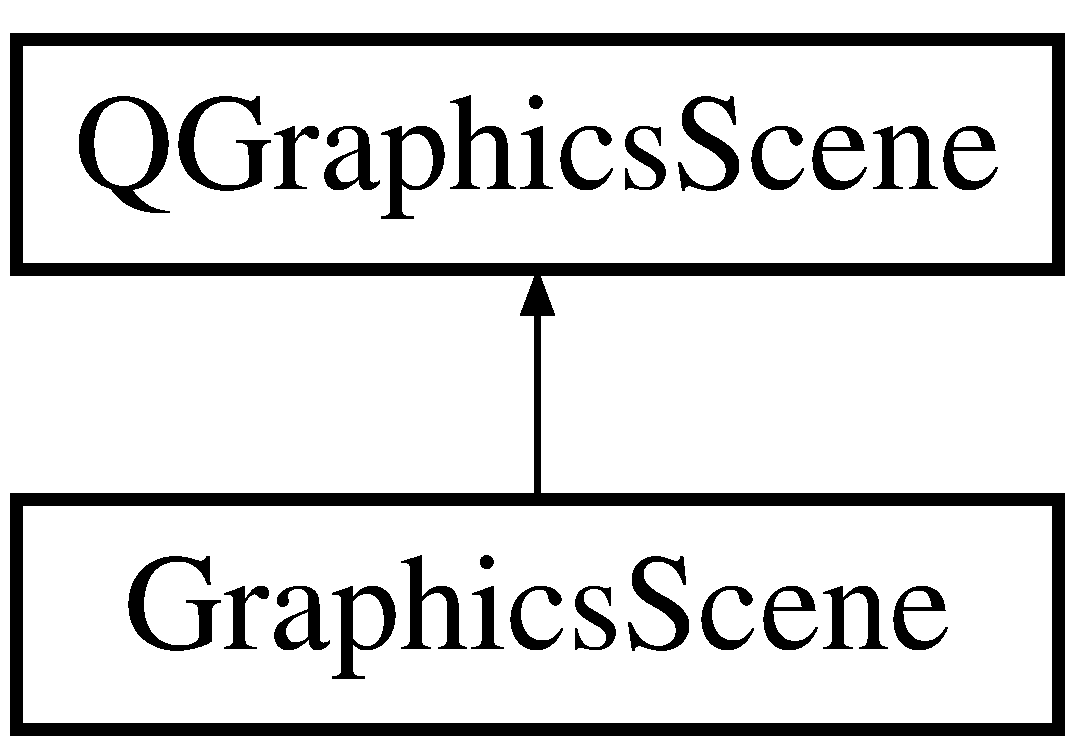
\includegraphics[height=2.000000cm]{class_graphics_scene}
\end{center}
\end{figure}
\subsection*{Signals}
\begin{DoxyCompactItemize}
\item 
void \hyperlink{class_graphics_scene_aee2d967bd98adf009edf0ecd08cec189}{send\+Mouse\+Position} (Q\+PointF mouse\+\_\+position)
\begin{DoxyCompactList}\small\item\em send\+Mouse\+Position -\/ Signal, dass die Positionsdaten des Cursors aussendet. \end{DoxyCompactList}\item 
void \hyperlink{class_graphics_scene_ac781d598feae85b0a0c6a90c30f914bd}{send\+Mouse\+Clicked\+Position} (Q\+PointF mouse\+\_\+clicked\+\_\+position)
\begin{DoxyCompactList}\small\item\em send\+Mouse\+Clicked\+Position -\/ Signal, dass die Positionsdaten des Cursors aussenden sobald geklickt wird. \end{DoxyCompactList}\end{DoxyCompactItemize}
\subsection*{Public Member Functions}
\begin{DoxyCompactItemize}
\item 
\hyperlink{class_graphics_scene_a5a6ac24fb693cce13e3d69c0c38311c9}{Graphics\+Scene} ()
\begin{DoxyCompactList}\small\item\em \hyperlink{class_graphics_scene_a5a6ac24fb693cce13e3d69c0c38311c9}{Graphics\+Scene\+::\+Graphics\+Scene}. Scene in der die Rechteck \& Kreis -\/ Objekte erstellt werden. \end{DoxyCompactList}\item 
void \hyperlink{class_graphics_scene_a68d455a648fe4a6717a1771c7fe04f31}{mouse\+Press\+Event} (Q\+Graphics\+Scene\+Mouse\+Event $\ast$mouse\+Event)
\begin{DoxyCompactList}\small\item\em mouse\+Press\+Event \end{DoxyCompactList}\item 
void \hyperlink{class_graphics_scene_aadc9534ab8b8fbb5e7c02a0b761c750a}{mouse\+Release\+Event} (Q\+Graphics\+Scene\+Mouse\+Event $\ast$mouse\+Event)
\begin{DoxyCompactList}\small\item\em mouse\+Release\+Event \end{DoxyCompactList}\item 
void \hyperlink{class_graphics_scene_a85927a0baa140f37d2c918866c6879f1}{mouse\+Move\+Event} (Q\+Graphics\+Scene\+Mouse\+Event $\ast$mouse\+Event)
\begin{DoxyCompactList}\small\item\em mouse\+Move\+Event \end{DoxyCompactList}\end{DoxyCompactItemize}
\subsection*{Protected Attributes}
\begin{DoxyCompactItemize}
\item 
\hyperlink{class_tools_ab031688a77e89a80ce8b5db7014684a3}{Tools\+::\+Draw\+Tool} \hyperlink{class_graphics_scene_aea13f23ba3e463916435ec72eb381207}{m\+\_\+active\+Tool}
\item 
\hyperlink{class_tools_a4b55b2ca4eef4d80ae1042233832bb8b}{Tools\+::\+Option\+Tool} \hyperlink{class_graphics_scene_ad17292fb79972e11c2a829da9baf3dca}{m\+\_\+active\+Option\+Tool}
\end{DoxyCompactItemize}


\subsection{Detailed Description}
The \hyperlink{class_graphics_scene}{Graphics\+Scene} class -\/ Klasse für die \hyperlink{class_graphics_scene}{Graphics\+Scene} abgeleitet von Q\+Graphics\+Scene. 

\subsection{Constructor \& Destructor Documentation}
\mbox{\Hypertarget{class_graphics_scene_a5a6ac24fb693cce13e3d69c0c38311c9}\label{class_graphics_scene_a5a6ac24fb693cce13e3d69c0c38311c9}} 
\index{Graphics\+Scene@{Graphics\+Scene}!Graphics\+Scene@{Graphics\+Scene}}
\index{Graphics\+Scene@{Graphics\+Scene}!Graphics\+Scene@{Graphics\+Scene}}
\subsubsection{\texorpdfstring{Graphics\+Scene()}{GraphicsScene()}}
{\footnotesize\ttfamily Graphics\+Scene\+::\+Graphics\+Scene (\begin{DoxyParamCaption}{ }\end{DoxyParamCaption})}



\hyperlink{class_graphics_scene_a5a6ac24fb693cce13e3d69c0c38311c9}{Graphics\+Scene\+::\+Graphics\+Scene}. Scene in der die Rechteck \& Kreis -\/ Objekte erstellt werden. 



\subsection{Member Function Documentation}
\mbox{\Hypertarget{class_graphics_scene_a85927a0baa140f37d2c918866c6879f1}\label{class_graphics_scene_a85927a0baa140f37d2c918866c6879f1}} 
\index{Graphics\+Scene@{Graphics\+Scene}!mouse\+Move\+Event@{mouse\+Move\+Event}}
\index{mouse\+Move\+Event@{mouse\+Move\+Event}!Graphics\+Scene@{Graphics\+Scene}}
\subsubsection{\texorpdfstring{mouse\+Move\+Event()}{mouseMoveEvent()}}
{\footnotesize\ttfamily void Graphics\+Scene\+::mouse\+Move\+Event (\begin{DoxyParamCaption}\item[{Q\+Graphics\+Scene\+Mouse\+Event $\ast$}]{mouse\+Event }\end{DoxyParamCaption})}



mouse\+Move\+Event 

\hyperlink{class_graphics_scene_a85927a0baa140f37d2c918866c6879f1}{Graphics\+Scene\+::mouse\+Move\+Event} -\/ Methode die ausgeführt wird wenn sich die Maus innerhalb der \hyperlink{class_graphics_scene}{Graphics\+Scene} bewegt.


\begin{DoxyParams}{Parameters}
{\em mouse\+Event} & \\
\hline
\end{DoxyParams}
$<$Sendet Signal aus mit den Positionsdaten des Cursors \mbox{\Hypertarget{class_graphics_scene_a68d455a648fe4a6717a1771c7fe04f31}\label{class_graphics_scene_a68d455a648fe4a6717a1771c7fe04f31}} 
\index{Graphics\+Scene@{Graphics\+Scene}!mouse\+Press\+Event@{mouse\+Press\+Event}}
\index{mouse\+Press\+Event@{mouse\+Press\+Event}!Graphics\+Scene@{Graphics\+Scene}}
\subsubsection{\texorpdfstring{mouse\+Press\+Event()}{mousePressEvent()}}
{\footnotesize\ttfamily void Graphics\+Scene\+::mouse\+Press\+Event (\begin{DoxyParamCaption}\item[{Q\+Graphics\+Scene\+Mouse\+Event $\ast$}]{mouse\+Event }\end{DoxyParamCaption})}



mouse\+Press\+Event 

\hyperlink{class_graphics_scene_a68d455a648fe4a6717a1771c7fe04f31}{Graphics\+Scene\+::mouse\+Press\+Event}.


\begin{DoxyParams}{Parameters}
{\em mouse\+Event} & \\
\hline
\end{DoxyParams}
button() gibt den Button zurück der das Event ausgelöst hat. Diese if -\/ Anweisung wird aufgerufen wenn die linke Maustaste gedrückt wird

Fall, sobald das \hyperlink{class_polygon}{Polygon} ausgwählt wurde und auf der Scene mit der Maus geklickt wird.\mbox{\Hypertarget{class_graphics_scene_aadc9534ab8b8fbb5e7c02a0b761c750a}\label{class_graphics_scene_aadc9534ab8b8fbb5e7c02a0b761c750a}} 
\index{Graphics\+Scene@{Graphics\+Scene}!mouse\+Release\+Event@{mouse\+Release\+Event}}
\index{mouse\+Release\+Event@{mouse\+Release\+Event}!Graphics\+Scene@{Graphics\+Scene}}
\subsubsection{\texorpdfstring{mouse\+Release\+Event()}{mouseReleaseEvent()}}
{\footnotesize\ttfamily void Graphics\+Scene\+::mouse\+Release\+Event (\begin{DoxyParamCaption}\item[{Q\+Graphics\+Scene\+Mouse\+Event $\ast$}]{mouse\+Event }\end{DoxyParamCaption})}



mouse\+Release\+Event 

\hyperlink{class_graphics_scene_aadc9534ab8b8fbb5e7c02a0b761c750a}{Graphics\+Scene\+::mouse\+Release\+Event}.


\begin{DoxyParams}{Parameters}
{\em mouse\+Event} & \\
\hline
\end{DoxyParams}
button() gibt den Button zurück der das Event ausgelöst hat. Wenn dieser Button der Linke Maus\+Button war dann wird der q\+Debug ausgegeben.\mbox{\Hypertarget{class_graphics_scene_ac781d598feae85b0a0c6a90c30f914bd}\label{class_graphics_scene_ac781d598feae85b0a0c6a90c30f914bd}} 
\index{Graphics\+Scene@{Graphics\+Scene}!send\+Mouse\+Clicked\+Position@{send\+Mouse\+Clicked\+Position}}
\index{send\+Mouse\+Clicked\+Position@{send\+Mouse\+Clicked\+Position}!Graphics\+Scene@{Graphics\+Scene}}
\subsubsection{\texorpdfstring{send\+Mouse\+Clicked\+Position}{sendMouseClickedPosition}}
{\footnotesize\ttfamily void Graphics\+Scene\+::send\+Mouse\+Clicked\+Position (\begin{DoxyParamCaption}\item[{Q\+PointF}]{mouse\+\_\+clicked\+\_\+position }\end{DoxyParamCaption})\hspace{0.3cm}{\ttfamily [signal]}}



send\+Mouse\+Clicked\+Position -\/ Signal, dass die Positionsdaten des Cursors aussenden sobald geklickt wird. 


\begin{DoxyParams}{Parameters}
{\em mouse\+\_\+clicked\+\_\+position} & \\
\hline
\end{DoxyParams}
\mbox{\Hypertarget{class_graphics_scene_aee2d967bd98adf009edf0ecd08cec189}\label{class_graphics_scene_aee2d967bd98adf009edf0ecd08cec189}} 
\index{Graphics\+Scene@{Graphics\+Scene}!send\+Mouse\+Position@{send\+Mouse\+Position}}
\index{send\+Mouse\+Position@{send\+Mouse\+Position}!Graphics\+Scene@{Graphics\+Scene}}
\subsubsection{\texorpdfstring{send\+Mouse\+Position}{sendMousePosition}}
{\footnotesize\ttfamily void Graphics\+Scene\+::send\+Mouse\+Position (\begin{DoxyParamCaption}\item[{Q\+PointF}]{mouse\+\_\+position }\end{DoxyParamCaption})\hspace{0.3cm}{\ttfamily [signal]}}



send\+Mouse\+Position -\/ Signal, dass die Positionsdaten des Cursors aussendet. 


\begin{DoxyParams}{Parameters}
{\em mouse\+\_\+position} & \\
\hline
\end{DoxyParams}


\subsection{Member Data Documentation}
\mbox{\Hypertarget{class_graphics_scene_ad17292fb79972e11c2a829da9baf3dca}\label{class_graphics_scene_ad17292fb79972e11c2a829da9baf3dca}} 
\index{Graphics\+Scene@{Graphics\+Scene}!m\+\_\+active\+Option\+Tool@{m\+\_\+active\+Option\+Tool}}
\index{m\+\_\+active\+Option\+Tool@{m\+\_\+active\+Option\+Tool}!Graphics\+Scene@{Graphics\+Scene}}
\subsubsection{\texorpdfstring{m\+\_\+active\+Option\+Tool}{m\_activeOptionTool}}
{\footnotesize\ttfamily \hyperlink{class_tools_a4b55b2ca4eef4d80ae1042233832bb8b}{Tools\+::\+Option\+Tool} Graphics\+Scene\+::m\+\_\+active\+Option\+Tool\hspace{0.3cm}{\ttfamily [protected]}}

\mbox{\Hypertarget{class_graphics_scene_aea13f23ba3e463916435ec72eb381207}\label{class_graphics_scene_aea13f23ba3e463916435ec72eb381207}} 
\index{Graphics\+Scene@{Graphics\+Scene}!m\+\_\+active\+Tool@{m\+\_\+active\+Tool}}
\index{m\+\_\+active\+Tool@{m\+\_\+active\+Tool}!Graphics\+Scene@{Graphics\+Scene}}
\subsubsection{\texorpdfstring{m\+\_\+active\+Tool}{m\_activeTool}}
{\footnotesize\ttfamily \hyperlink{class_tools_ab031688a77e89a80ce8b5db7014684a3}{Tools\+::\+Draw\+Tool} Graphics\+Scene\+::m\+\_\+active\+Tool\hspace{0.3cm}{\ttfamily [protected]}}



The documentation for this class was generated from the following files\+:\begin{DoxyCompactItemize}
\item 
C\+:/\+Users/tranb/\+Desktop/\+Sciebo/\+Studium/\+Qt Projekte/\+Graphic\+Obj/\hyperlink{graphicsscene_8h}{graphicsscene.\+h}\item 
C\+:/\+Users/tranb/\+Desktop/\+Sciebo/\+Studium/\+Qt Projekte/\+Graphic\+Obj/\hyperlink{graphicsscene_8cpp}{graphicsscene.\+cpp}\end{DoxyCompactItemize}

\hypertarget{class_main_window}{}\section{Main\+Window Class Reference}
\label{class_main_window}\index{Main\+Window@{Main\+Window}}


The \hyperlink{class_main_window}{Main\+Window} class -\/ \hyperlink{class_main_window}{Main\+Window} Klasse.  




{\ttfamily \#include $<$mainwindow.\+h$>$}

Inheritance diagram for Main\+Window\+:\begin{figure}[H]
\begin{center}
\leavevmode
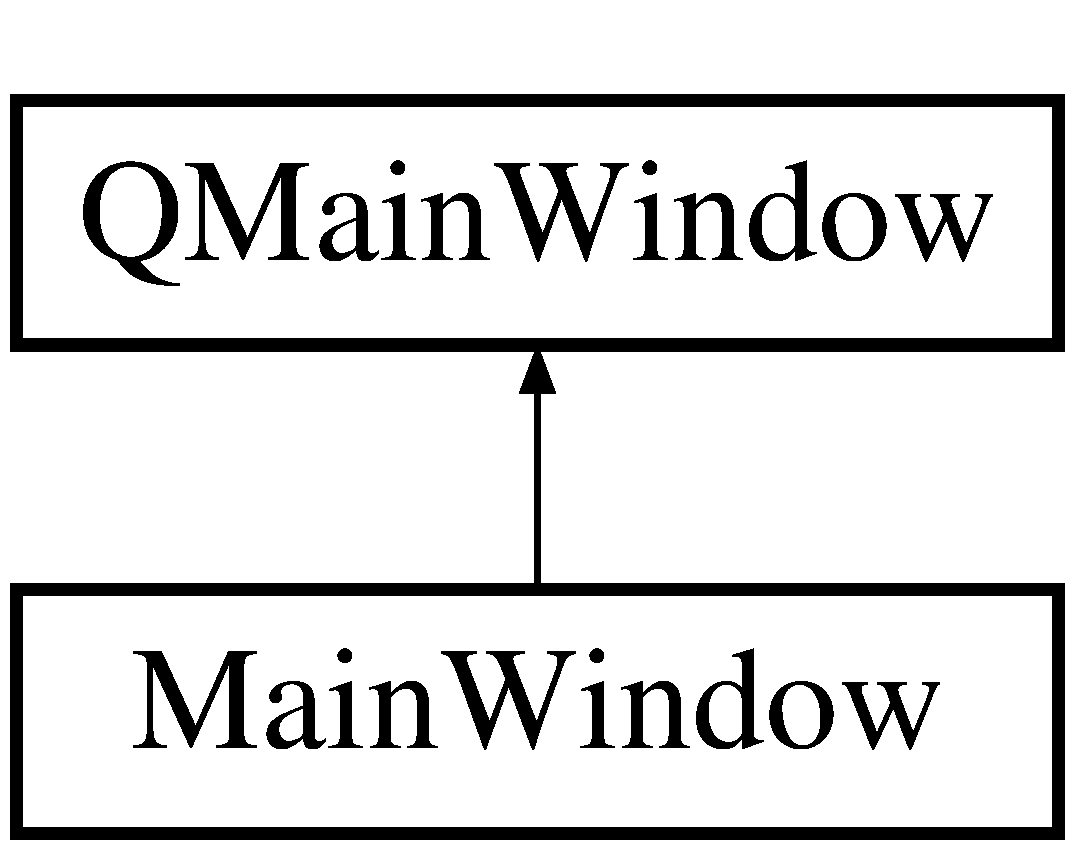
\includegraphics[height=2.000000cm]{class_main_window}
\end{center}
\end{figure}
\subsection*{Public Slots}
\begin{DoxyCompactItemize}
\item 
void \hyperlink{class_main_window_a965877b0ba4c3f18035232a9eb7b98e0}{recieve\+Mouse\+Position} (Q\+PointF mouse\+\_\+position)
\begin{DoxyCompactList}\small\item\em recieve\+Mouse\+Position -\/ Slot für das Empfangen der Maus Position. \end{DoxyCompactList}\item 
void \hyperlink{class_main_window_a3ea2675e6bd470873d7569db47a5bd2a}{recieve\+Mouse\+Clicked\+Position} (Q\+PointF mouse\+\_\+clicked\+\_\+position)
\begin{DoxyCompactList}\small\item\em recieve\+Mouse\+Clicked\+Position -\/ Slot für das Empfangen der Maus Position, wenn auf der Scene geklickt wird. \end{DoxyCompactList}\item 
void \hyperlink{class_main_window_aee13312aef8f1fc2a4c7ff2f8837234c}{recieve\+Focused\+Item} (qreal x, qreal y, qreal height, qreal width)
\end{DoxyCompactItemize}
\subsection*{Public Member Functions}
\begin{DoxyCompactItemize}
\item 
\hyperlink{class_main_window_a8b244be8b7b7db1b08de2a2acb9409db}{Main\+Window} (Q\+Widget $\ast$parent=0)
\begin{DoxyCompactList}\small\item\em \hyperlink{class_main_window}{Main\+Window}. \end{DoxyCompactList}\item 
\hyperlink{class_main_window_ae98d00a93bc118200eeef9f9bba1dba7}{$\sim$\+Main\+Window} ()
\begin{DoxyCompactList}\small\item\em \hyperlink{class_main_window_ae98d00a93bc118200eeef9f9bba1dba7}{Main\+Window\+::$\sim$\+Main\+Window} ist der Dekonstruktor. \end{DoxyCompactList}\end{DoxyCompactItemize}


\subsection{Detailed Description}
The \hyperlink{class_main_window}{Main\+Window} class -\/ \hyperlink{class_main_window}{Main\+Window} Klasse. 

\subsection{Constructor \& Destructor Documentation}
\mbox{\Hypertarget{class_main_window_a8b244be8b7b7db1b08de2a2acb9409db}\label{class_main_window_a8b244be8b7b7db1b08de2a2acb9409db}} 
\index{Main\+Window@{Main\+Window}!Main\+Window@{Main\+Window}}
\index{Main\+Window@{Main\+Window}!Main\+Window@{Main\+Window}}
\subsubsection{\texorpdfstring{Main\+Window()}{MainWindow()}}
{\footnotesize\ttfamily Main\+Window\+::\+Main\+Window (\begin{DoxyParamCaption}\item[{Q\+Widget $\ast$}]{parent = {\ttfamily 0} }\end{DoxyParamCaption})\hspace{0.3cm}{\ttfamily [explicit]}}



\hyperlink{class_main_window}{Main\+Window}. 

\hyperlink{class_main_window_a8b244be8b7b7db1b08de2a2acb9409db}{Main\+Window\+::\+Main\+Window}.


\begin{DoxyParams}{Parameters}
{\em parent} & \\
\hline
\end{DoxyParams}
$<$User Interface wird aufgerufen

$<$\hyperlink{class_tools}{Tools} -\/ Objekt wird erstellt und Default -\/ Werte werden gesetzt.

$<$Setzt Systemtypisches Icon für Menüpunkt \char`\"{}\+Open\char`\"{}

$<$Setzt Systemtypisches Icon für Menüpunkt \char`\"{}\+Save\char`\"{}

$<$Setzt Systemtypische Shortcut für den Menüpunkt \char`\"{}\+Open\char`\"{}

$<$Setzt Systemtypische Shortcut für den Menüpunkt \char`\"{}\+Save\char`\"{}

$<$Setzt Systemtypische Shortcut für den Menüpunkt \char`\"{}\+Print\char`\"{}

Damit das hier funktioniert, muss erst ein Label dem Central\+Widget hinzugefügt werden. (im G\+UI -\/ Creator)

$<$Das Label wird hiermit der Statusbar beigefügt.

$<$Graphic\+Scene -\/ Objekt wird erstellt

$<$Das Graphic\+Scene -\/ Objekt wird dem graphics\+View -\/ Widget übergeben

$<$Größe der Graphic\+Scene wird gesetzt.

$<$Graut Add\+Object -\/ Button aus.

$<$Macht Positionen / Dimensionen Feld unsichtbar (Default)

$<$Graut Menüpunkt Add\+Object aus

connect Verbindung zwischen dem tool\+Object aus \hyperlink{class_main_window}{Main\+Window} und dem eigenem Widget für Zeichenwerkzeuge Richtung\+: tool\+Object zu eigenem Widget.

connect Verbindung zwischen dem eigenem Widget für Zeichenwerkzeuge und dem tool\+Object aus \hyperlink{class_main_window}{Main\+Window} Richtung\+: eigenes Widget zu tool\+Object

connect Verbindung zwischen tool\+Object und dem eigenem Widget zur Farbauswahl für die Rahmenfarbe Richtung\+: tool\+Object zu eigenem Widget

connect Verbindung zwischen eigenem Widget zur Farbauswahl für die Rahmenfarbe und dem tool\+Object Richtung\+: eigenes Widget zu tool\+Object

connect Verbindung zwischen dem tool\+Object und dem eigenem Widget zur Farbauswahl für die Füllfarbe Richtung\+: tool\+Object zu eigenem Widget

connect Verbindung zwischen dem eigenem Widget für die Füllfarbe zu dem tool\+Object Richtung\+: eigenes Widget zu tool\+Object.

connect Verbindung zwischen dem eigenem Widget und dem \hyperlink{class_main_window}{Main\+Window}. Richtung\+: eigenes Widget zu \hyperlink{class_main_window}{Main\+Window}.

connect Verbindung zwischen der Scene und dem \hyperlink{class_main_window}{Main\+Window} (Cursor\+Koordinaten werden an Statusbar gesendet) Richtung\+: Scene zu \hyperlink{class_main_window}{Main\+Window}

connect Verbindung zwischen dem \hyperlink{class_drawing_tool_selector}{Drawing\+Tool\+Selector} und der Graphicsscene. Richtung\+: \hyperlink{class_drawing_tool_selector}{Drawing\+Tool\+Selector} zu Scene

connect Verbindung zwischen der Scene und dem \hyperlink{class_main_window}{Main\+Window} für die Mausposition wenn mit der Maus auf die Scene geklickt wird. Richtung\+: Scene zu \hyperlink{class_main_window}{Main\+Window} (funktioniert nur, wenn Polygon\+Tool ausgewählt wurde.)

connect Verbindung zwischen dem Drawin\+Tool\+Selector und dem Tool\+Object für die Wahl zwischen Grundriss und Moebel. Richtung\+: Drawingtool\+Selector zu tool\+Object\mbox{\Hypertarget{class_main_window_ae98d00a93bc118200eeef9f9bba1dba7}\label{class_main_window_ae98d00a93bc118200eeef9f9bba1dba7}} 
\index{Main\+Window@{Main\+Window}!````~Main\+Window@{$\sim$\+Main\+Window}}
\index{````~Main\+Window@{$\sim$\+Main\+Window}!Main\+Window@{Main\+Window}}
\subsubsection{\texorpdfstring{$\sim$\+Main\+Window()}{~MainWindow()}}
{\footnotesize\ttfamily Main\+Window\+::$\sim$\+Main\+Window (\begin{DoxyParamCaption}{ }\end{DoxyParamCaption})}



\hyperlink{class_main_window_ae98d00a93bc118200eeef9f9bba1dba7}{Main\+Window\+::$\sim$\+Main\+Window} ist der Dekonstruktor. 



\subsection{Member Function Documentation}
\mbox{\Hypertarget{class_main_window_aee13312aef8f1fc2a4c7ff2f8837234c}\label{class_main_window_aee13312aef8f1fc2a4c7ff2f8837234c}} 
\index{Main\+Window@{Main\+Window}!recieve\+Focused\+Item@{recieve\+Focused\+Item}}
\index{recieve\+Focused\+Item@{recieve\+Focused\+Item}!Main\+Window@{Main\+Window}}
\subsubsection{\texorpdfstring{recieve\+Focused\+Item}{recieveFocusedItem}}
{\footnotesize\ttfamily void Main\+Window\+::recieve\+Focused\+Item (\begin{DoxyParamCaption}\item[{qreal}]{x,  }\item[{qreal}]{y,  }\item[{qreal}]{height,  }\item[{qreal}]{width }\end{DoxyParamCaption})\hspace{0.3cm}{\ttfamily [slot]}}

\mbox{\Hypertarget{class_main_window_a3ea2675e6bd470873d7569db47a5bd2a}\label{class_main_window_a3ea2675e6bd470873d7569db47a5bd2a}} 
\index{Main\+Window@{Main\+Window}!recieve\+Mouse\+Clicked\+Position@{recieve\+Mouse\+Clicked\+Position}}
\index{recieve\+Mouse\+Clicked\+Position@{recieve\+Mouse\+Clicked\+Position}!Main\+Window@{Main\+Window}}
\subsubsection{\texorpdfstring{recieve\+Mouse\+Clicked\+Position}{recieveMouseClickedPosition}}
{\footnotesize\ttfamily void Main\+Window\+::recieve\+Mouse\+Clicked\+Position (\begin{DoxyParamCaption}\item[{Q\+PointF}]{mouse\+\_\+clicked\+\_\+position }\end{DoxyParamCaption})\hspace{0.3cm}{\ttfamily [slot]}}



recieve\+Mouse\+Clicked\+Position -\/ Slot für das Empfangen der Maus Position, wenn auf der Scene geklickt wird. 

\hyperlink{class_main_window_a3ea2675e6bd470873d7569db47a5bd2a}{Main\+Window\+::recieve\+Mouse\+Clicked\+Position} -\/ Methode, um die gewünschten Eckpunkte des Polygons auf die Scene zu malen und die Punkte in die Polygon\+Liste hinzuzufügen. Diese wird später zum Verbinden der Punkte benötigt.


\begin{DoxyParams}{Parameters}
{\em mouse\+\_\+clicked\+\_\+position} & \\
\hline
\end{DoxyParams}
$<$Setzt einen Punkt an der gewünschten Position

$<$Fügt die Koordinaten der \char`\"{}\+Hilfskreise\char`\"{} in die Liste ein.

$<$Fügt die \char`\"{}\+Hilfskreise\char`\"{} in die dafür vorhandene Liste.

$<$Malt den Punkt auf die Scene \mbox{\Hypertarget{class_main_window_a965877b0ba4c3f18035232a9eb7b98e0}\label{class_main_window_a965877b0ba4c3f18035232a9eb7b98e0}} 
\index{Main\+Window@{Main\+Window}!recieve\+Mouse\+Position@{recieve\+Mouse\+Position}}
\index{recieve\+Mouse\+Position@{recieve\+Mouse\+Position}!Main\+Window@{Main\+Window}}
\subsubsection{\texorpdfstring{recieve\+Mouse\+Position}{recieveMousePosition}}
{\footnotesize\ttfamily void Main\+Window\+::recieve\+Mouse\+Position (\begin{DoxyParamCaption}\item[{Q\+PointF}]{mouse\+\_\+position }\end{DoxyParamCaption})\hspace{0.3cm}{\ttfamily [slot]}}



recieve\+Mouse\+Position -\/ Slot für das Empfangen der Maus Position. 

\hyperlink{class_main_window_a965877b0ba4c3f18035232a9eb7b98e0}{Main\+Window\+::recieve\+Mouse\+Position}.


\begin{DoxyParams}{Parameters}
{\em mouse\+\_\+position} & \\
\hline
{\em mouse\+\_\+position} & Der Slot der vom dem Signal(send\+Mouse\+Position) aus Graphicsscene die Mouse Position empfängt. Dem Label auf der Statusbar werden dann die Maus Positionen beigefügt. \\
\hline
\end{DoxyParams}
$<$Setzt den Text des Labels

$<$Fügt x\+Koordinate hinzu

$<$Fügt y\+Koordinate hinzu 

The documentation for this class was generated from the following files\+:\begin{DoxyCompactItemize}
\item 
C\+:/\+Users/tranb/\+Desktop/\+Sciebo/\+Studium/\+Qt Projekte/\+Graphic\+Obj/\hyperlink{mainwindow_8h}{mainwindow.\+h}\item 
C\+:/\+Users/tranb/\+Desktop/\+Sciebo/\+Studium/\+Qt Projekte/\+Graphic\+Obj/\hyperlink{mainwindow_8cpp}{mainwindow.\+cpp}\end{DoxyCompactItemize}

\hypertarget{class_object_options}{}\section{Object\+Options Class Reference}
\label{class_object_options}\index{Object\+Options@{Object\+Options}}


The \hyperlink{class_object_options}{Object\+Options} class -\/ Eigenes zusammengestelltes Widget für die Dimensonen und Position.  




{\ttfamily \#include $<$objectoptions.\+h$>$}

Inheritance diagram for Object\+Options\+:\begin{figure}[H]
\begin{center}
\leavevmode
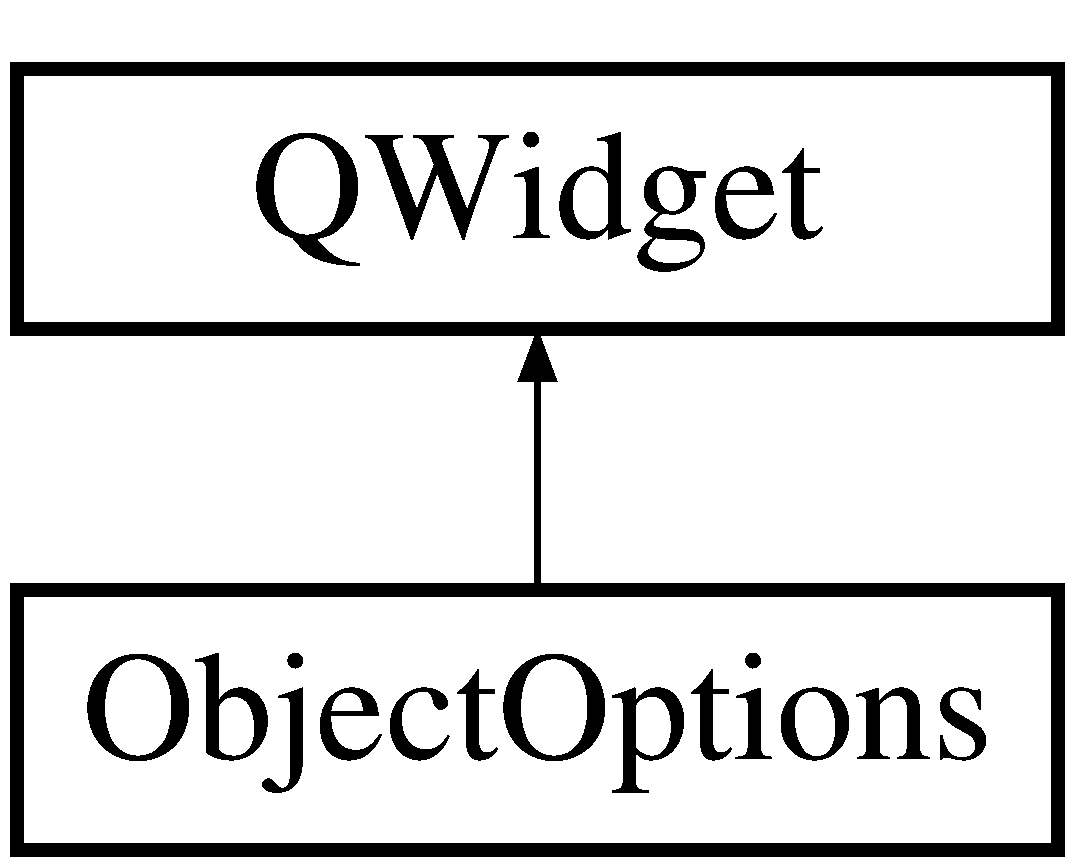
\includegraphics[height=2.000000cm]{class_object_options}
\end{center}
\end{figure}
\subsection*{Public Member Functions}
\begin{DoxyCompactItemize}
\item 
\hyperlink{class_object_options_aec863b929bf4ccba84210b58ab23e530}{Object\+Options} (Q\+Widget $\ast$parent=0)
\item 
\hyperlink{class_object_options_a93a5c0da34ad8420c19b65d76296f9c0}{$\sim$\+Object\+Options} ()
\item 
int \hyperlink{class_object_options_a738e07899e3eff5aeb2f998bf527b804}{xkoord} () const
\begin{DoxyCompactList}\small\item\em Getter Methode für m\+\_\+xkoord. \end{DoxyCompactList}\item 
int \hyperlink{class_object_options_a3306979371a1f706724d2e5a449d3f72}{ykoord} () const
\begin{DoxyCompactList}\small\item\em Getter Methode für m\+\_\+ykoord. \end{DoxyCompactList}\item 
int \hyperlink{class_object_options_af520e91fb7c4980c04e21f1a306264b1}{height} () const
\begin{DoxyCompactList}\small\item\em Getter Methode für m\+\_\+height. \end{DoxyCompactList}\item 
int \hyperlink{class_object_options_a57594cc38acb8ebf466bb41538a35a8b}{width} () const
\begin{DoxyCompactList}\small\item\em Getter Methode für m\+\_\+width. \end{DoxyCompactList}\item 
void \hyperlink{class_object_options_acdb5c1b9952fda67ac8393055acfd756}{set\+Xkoord} (int \hyperlink{class_object_options_a738e07899e3eff5aeb2f998bf527b804}{xkoord})
\item 
void \hyperlink{class_object_options_a32b59030cadbd75a09ed0056df03d342}{set\+Ykoord} (int \hyperlink{class_object_options_a3306979371a1f706724d2e5a449d3f72}{ykoord})
\item 
void \hyperlink{class_object_options_a7e490c997a49ddd45317598dc851f473}{set\+Height} (int \hyperlink{class_object_options_af520e91fb7c4980c04e21f1a306264b1}{height})
\item 
void \hyperlink{class_object_options_a33cd9c2ae781069d22babab1ac346af9}{set\+Width} (int \hyperlink{class_object_options_a57594cc38acb8ebf466bb41538a35a8b}{width})
\end{DoxyCompactItemize}


\subsection{Detailed Description}
The \hyperlink{class_object_options}{Object\+Options} class -\/ Eigenes zusammengestelltes Widget für die Dimensonen und Position. 

\subsection{Constructor \& Destructor Documentation}
\mbox{\Hypertarget{class_object_options_aec863b929bf4ccba84210b58ab23e530}\label{class_object_options_aec863b929bf4ccba84210b58ab23e530}} 
\index{Object\+Options@{Object\+Options}!Object\+Options@{Object\+Options}}
\index{Object\+Options@{Object\+Options}!Object\+Options@{Object\+Options}}
\subsubsection{\texorpdfstring{Object\+Options()}{ObjectOptions()}}
{\footnotesize\ttfamily Object\+Options\+::\+Object\+Options (\begin{DoxyParamCaption}\item[{Q\+Widget $\ast$}]{parent = {\ttfamily 0} }\end{DoxyParamCaption})\hspace{0.3cm}{\ttfamily [explicit]}}

Hier werden Default -\/ Werte für die einzelnen Member -\/ Variablen gesetzt. Damit auch wenn beim Position/\+Dimensionen Feld nichts eingegeben wird bei manchen optionen das gewählte Objekt trotzdem gezeichnet werden kann.\mbox{\Hypertarget{class_object_options_a93a5c0da34ad8420c19b65d76296f9c0}\label{class_object_options_a93a5c0da34ad8420c19b65d76296f9c0}} 
\index{Object\+Options@{Object\+Options}!````~Object\+Options@{$\sim$\+Object\+Options}}
\index{````~Object\+Options@{$\sim$\+Object\+Options}!Object\+Options@{Object\+Options}}
\subsubsection{\texorpdfstring{$\sim$\+Object\+Options()}{~ObjectOptions()}}
{\footnotesize\ttfamily Object\+Options\+::$\sim$\+Object\+Options (\begin{DoxyParamCaption}{ }\end{DoxyParamCaption})}



\subsection{Member Function Documentation}
\mbox{\Hypertarget{class_object_options_af520e91fb7c4980c04e21f1a306264b1}\label{class_object_options_af520e91fb7c4980c04e21f1a306264b1}} 
\index{Object\+Options@{Object\+Options}!height@{height}}
\index{height@{height}!Object\+Options@{Object\+Options}}
\subsubsection{\texorpdfstring{height()}{height()}}
{\footnotesize\ttfamily int Object\+Options\+::height (\begin{DoxyParamCaption}{ }\end{DoxyParamCaption}) const}



Getter Methode für m\+\_\+height. 

\hyperlink{class_object_options_af520e91fb7c4980c04e21f1a306264b1}{Object\+Options\+::height} -\/ Getter -\/ Methode für m\+\_\+height.

\begin{DoxyReturn}{Returns}
m\+\_\+height


\end{DoxyReturn}
\mbox{\Hypertarget{class_object_options_a7e490c997a49ddd45317598dc851f473}\label{class_object_options_a7e490c997a49ddd45317598dc851f473}} 
\index{Object\+Options@{Object\+Options}!set\+Height@{set\+Height}}
\index{set\+Height@{set\+Height}!Object\+Options@{Object\+Options}}
\subsubsection{\texorpdfstring{set\+Height()}{setHeight()}}
{\footnotesize\ttfamily void Object\+Options\+::set\+Height (\begin{DoxyParamCaption}\item[{int}]{height }\end{DoxyParamCaption})}

\mbox{\Hypertarget{class_object_options_a33cd9c2ae781069d22babab1ac346af9}\label{class_object_options_a33cd9c2ae781069d22babab1ac346af9}} 
\index{Object\+Options@{Object\+Options}!set\+Width@{set\+Width}}
\index{set\+Width@{set\+Width}!Object\+Options@{Object\+Options}}
\subsubsection{\texorpdfstring{set\+Width()}{setWidth()}}
{\footnotesize\ttfamily void Object\+Options\+::set\+Width (\begin{DoxyParamCaption}\item[{int}]{width }\end{DoxyParamCaption})}

\mbox{\Hypertarget{class_object_options_acdb5c1b9952fda67ac8393055acfd756}\label{class_object_options_acdb5c1b9952fda67ac8393055acfd756}} 
\index{Object\+Options@{Object\+Options}!set\+Xkoord@{set\+Xkoord}}
\index{set\+Xkoord@{set\+Xkoord}!Object\+Options@{Object\+Options}}
\subsubsection{\texorpdfstring{set\+Xkoord()}{setXkoord()}}
{\footnotesize\ttfamily void Object\+Options\+::set\+Xkoord (\begin{DoxyParamCaption}\item[{int}]{xkoord }\end{DoxyParamCaption})}

\mbox{\Hypertarget{class_object_options_a32b59030cadbd75a09ed0056df03d342}\label{class_object_options_a32b59030cadbd75a09ed0056df03d342}} 
\index{Object\+Options@{Object\+Options}!set\+Ykoord@{set\+Ykoord}}
\index{set\+Ykoord@{set\+Ykoord}!Object\+Options@{Object\+Options}}
\subsubsection{\texorpdfstring{set\+Ykoord()}{setYkoord()}}
{\footnotesize\ttfamily void Object\+Options\+::set\+Ykoord (\begin{DoxyParamCaption}\item[{int}]{ykoord }\end{DoxyParamCaption})}

\mbox{\Hypertarget{class_object_options_a57594cc38acb8ebf466bb41538a35a8b}\label{class_object_options_a57594cc38acb8ebf466bb41538a35a8b}} 
\index{Object\+Options@{Object\+Options}!width@{width}}
\index{width@{width}!Object\+Options@{Object\+Options}}
\subsubsection{\texorpdfstring{width()}{width()}}
{\footnotesize\ttfamily int Object\+Options\+::width (\begin{DoxyParamCaption}{ }\end{DoxyParamCaption}) const}



Getter Methode für m\+\_\+width. 

\hyperlink{class_object_options_a57594cc38acb8ebf466bb41538a35a8b}{Object\+Options\+::width} -\/ Getter -\/ Methode für m\+\_\+width.

\begin{DoxyReturn}{Returns}
m\+\_\+width


\end{DoxyReturn}
\mbox{\Hypertarget{class_object_options_a738e07899e3eff5aeb2f998bf527b804}\label{class_object_options_a738e07899e3eff5aeb2f998bf527b804}} 
\index{Object\+Options@{Object\+Options}!xkoord@{xkoord}}
\index{xkoord@{xkoord}!Object\+Options@{Object\+Options}}
\subsubsection{\texorpdfstring{xkoord()}{xkoord()}}
{\footnotesize\ttfamily int Object\+Options\+::xkoord (\begin{DoxyParamCaption}{ }\end{DoxyParamCaption}) const}



Getter Methode für m\+\_\+xkoord. 

\hyperlink{class_object_options_a738e07899e3eff5aeb2f998bf527b804}{Object\+Options\+::xkoord} -\/ Getter -\/ Methode für m\+\_\+xkoord.

\begin{DoxyReturn}{Returns}
m\+\_\+xkoord


\end{DoxyReturn}
\mbox{\Hypertarget{class_object_options_a3306979371a1f706724d2e5a449d3f72}\label{class_object_options_a3306979371a1f706724d2e5a449d3f72}} 
\index{Object\+Options@{Object\+Options}!ykoord@{ykoord}}
\index{ykoord@{ykoord}!Object\+Options@{Object\+Options}}
\subsubsection{\texorpdfstring{ykoord()}{ykoord()}}
{\footnotesize\ttfamily int Object\+Options\+::ykoord (\begin{DoxyParamCaption}{ }\end{DoxyParamCaption}) const}



Getter Methode für m\+\_\+ykoord. 

\hyperlink{class_object_options_a3306979371a1f706724d2e5a449d3f72}{Object\+Options\+::ykoord} -\/ Getter -\/ Methode für m\+\_\+ykoord.

\begin{DoxyReturn}{Returns}
m\+\_\+ykoord


\end{DoxyReturn}


The documentation for this class was generated from the following files\+:\begin{DoxyCompactItemize}
\item 
C\+:/\+Users/tranb/\+Desktop/\+Sciebo/\+Studium/\+Qt Projekte/\+Graphic\+Obj/\hyperlink{objectoptions_8h}{objectoptions.\+h}\item 
C\+:/\+Users/tranb/\+Desktop/\+Sciebo/\+Studium/\+Qt Projekte/\+Graphic\+Obj/\hyperlink{objectoptions_8cpp}{objectoptions.\+cpp}\end{DoxyCompactItemize}

\hypertarget{class_polygon}{}\section{Polygon Class Reference}
\label{class_polygon}\index{Polygon@{Polygon}}


The \hyperlink{class_polygon}{Polygon} class -\/ Klasse für das \hyperlink{class_polygon}{Polygon} Objekt abgeleitet von Graphic Objekt.  




{\ttfamily \#include $<$polygon.\+h$>$}

Inheritance diagram for Polygon\+:\begin{figure}[H]
\begin{center}
\leavevmode
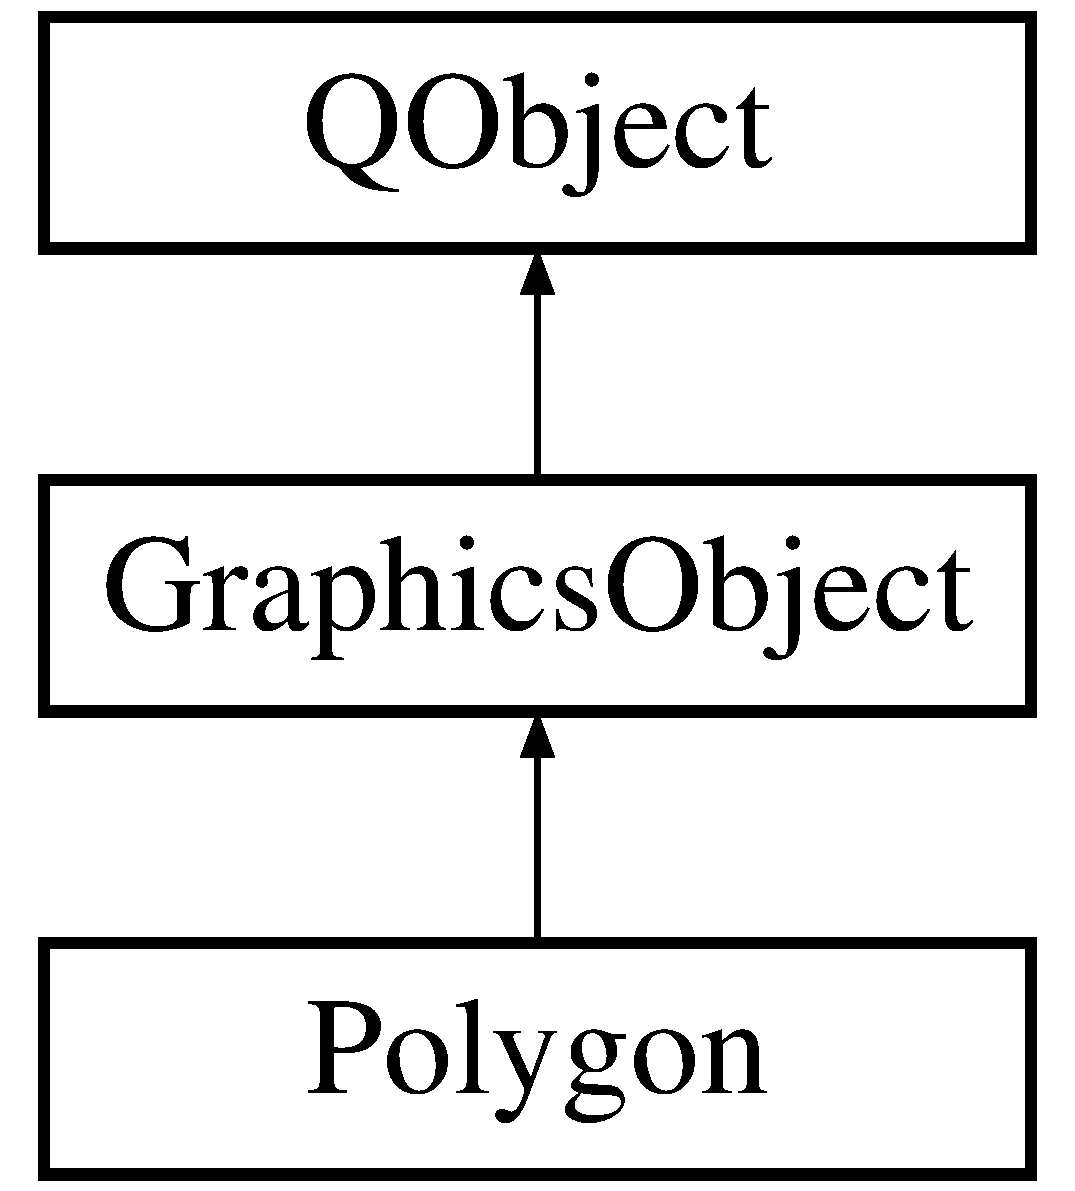
\includegraphics[height=3.000000cm]{class_polygon}
\end{center}
\end{figure}
\subsection*{Public Member Functions}
\begin{DoxyCompactItemize}
\item 
\hyperlink{class_polygon_acca8d3957dfbd44bb27c4519d2bfeb83}{Polygon} (Q\+Object $\ast$parent=nullptr)
\begin{DoxyCompactList}\small\item\em \hyperlink{class_polygon}{Polygon} -\/ Default Konstruktor für das \hyperlink{class_polygon}{Polygon} Objekt. \end{DoxyCompactList}\item 
\hyperlink{class_polygon_ace39c67107966db12e13a183f496c3b0}{$\sim$\+Polygon} ()
\begin{DoxyCompactList}\small\item\em \hyperlink{class_polygon}{Polygon} -\/ Destruktor. \end{DoxyCompactList}\item 
\hyperlink{class_polygon_a848d8c9194ace0906ae31bb9c26e3829}{Polygon} (Q\+Polygon polygon, Q\+Color pen, Q\+Color brush)
\begin{DoxyCompactList}\small\item\em \hyperlink{class_polygon}{Polygon} -\/ Selbst erstellter Konstruktor für das \hyperlink{class_polygon}{Polygon} Objekt. \end{DoxyCompactList}\item 
virtual Q\+Abstract\+Graphics\+Shape\+Item $\ast$ \hyperlink{class_polygon_aebf0f177dbc4da17a1822be5a0063b25}{graphic\+Shape\+Item} () const
\begin{DoxyCompactList}\small\item\em graphic\+Shape\+Item -\/ Gibt das Q\+Graphics\+Poygon\+Item zurück. \end{DoxyCompactList}\item 
virtual Q\+String \hyperlink{class_polygon_a588df36c92bfa626e0a16acb07162fa3}{to\+String} ()
\begin{DoxyCompactList}\small\item\em to\+String -\/ Methode für das \hyperlink{class_polygon}{Polygon} Objekt. \end{DoxyCompactList}\end{DoxyCompactItemize}
\subsection*{Protected Attributes}
\begin{DoxyCompactItemize}
\item 
Q\+Graphics\+Polygon\+Item $\ast$ \hyperlink{class_polygon_a464037e9e2eb2a1fa131eed357d02f83}{m\+\_\+graphics\+Polygon}
\end{DoxyCompactItemize}
\subsection*{Static Protected Attributes}
\begin{DoxyCompactItemize}
\item 
static unsigned long \hyperlink{class_polygon_a20f77e208065a18ac17b5b0cd5bd0dce}{m\+\_\+polygon\+Counter} = 0
\end{DoxyCompactItemize}


\subsection{Detailed Description}
The \hyperlink{class_polygon}{Polygon} class -\/ Klasse für das \hyperlink{class_polygon}{Polygon} Objekt abgeleitet von Graphic Objekt. 

\subsection{Constructor \& Destructor Documentation}
\mbox{\Hypertarget{class_polygon_acca8d3957dfbd44bb27c4519d2bfeb83}\label{class_polygon_acca8d3957dfbd44bb27c4519d2bfeb83}} 
\index{Polygon@{Polygon}!Polygon@{Polygon}}
\index{Polygon@{Polygon}!Polygon@{Polygon}}
\subsubsection{\texorpdfstring{Polygon()}{Polygon()}\hspace{0.1cm}{\footnotesize\ttfamily [1/2]}}
{\footnotesize\ttfamily Polygon\+::\+Polygon (\begin{DoxyParamCaption}\item[{Q\+Object $\ast$}]{parent = {\ttfamily nullptr} }\end{DoxyParamCaption})}



\hyperlink{class_polygon}{Polygon} -\/ Default Konstruktor für das \hyperlink{class_polygon}{Polygon} Objekt. 

\hyperlink{class_polygon_acca8d3957dfbd44bb27c4519d2bfeb83}{Polygon\+::\+Polygon} -\/ Default Konstrukor für das \hyperlink{class_polygon}{Polygon} Objekt.


\begin{DoxyParams}{Parameters}
{\em parent} & \\
\hline
\end{DoxyParams}
\mbox{\Hypertarget{class_polygon_ace39c67107966db12e13a183f496c3b0}\label{class_polygon_ace39c67107966db12e13a183f496c3b0}} 
\index{Polygon@{Polygon}!````~Polygon@{$\sim$\+Polygon}}
\index{````~Polygon@{$\sim$\+Polygon}!Polygon@{Polygon}}
\subsubsection{\texorpdfstring{$\sim$\+Polygon()}{~Polygon()}}
{\footnotesize\ttfamily Polygon\+::$\sim$\+Polygon (\begin{DoxyParamCaption}{ }\end{DoxyParamCaption})}



\hyperlink{class_polygon}{Polygon} -\/ Destruktor. 

\hyperlink{class_polygon_ace39c67107966db12e13a183f496c3b0}{Polygon\+::$\sim$\+Polygon} -\/ Destruktor für das \hyperlink{class_polygon}{Polygon} Objekt. \mbox{\Hypertarget{class_polygon_a848d8c9194ace0906ae31bb9c26e3829}\label{class_polygon_a848d8c9194ace0906ae31bb9c26e3829}} 
\index{Polygon@{Polygon}!Polygon@{Polygon}}
\index{Polygon@{Polygon}!Polygon@{Polygon}}
\subsubsection{\texorpdfstring{Polygon()}{Polygon()}\hspace{0.1cm}{\footnotesize\ttfamily [2/2]}}
{\footnotesize\ttfamily Polygon\+::\+Polygon (\begin{DoxyParamCaption}\item[{Q\+Polygon}]{polygon,  }\item[{Q\+Color}]{pen,  }\item[{Q\+Color}]{brush }\end{DoxyParamCaption})}



\hyperlink{class_polygon}{Polygon} -\/ Selbst erstellter Konstruktor für das \hyperlink{class_polygon}{Polygon} Objekt. 

\hyperlink{class_polygon_acca8d3957dfbd44bb27c4519d2bfeb83}{Polygon\+::\+Polygon} -\/ selbst erstellter Konstruktor für das \hyperlink{class_polygon}{Polygon} Objekt.


\begin{DoxyParams}{Parameters}
{\em polygon} & \\
\hline
{\em pen} & \\
\hline
{\em brush} & \\
\hline
\end{DoxyParams}


\subsection{Member Function Documentation}
\mbox{\Hypertarget{class_polygon_aebf0f177dbc4da17a1822be5a0063b25}\label{class_polygon_aebf0f177dbc4da17a1822be5a0063b25}} 
\index{Polygon@{Polygon}!graphic\+Shape\+Item@{graphic\+Shape\+Item}}
\index{graphic\+Shape\+Item@{graphic\+Shape\+Item}!Polygon@{Polygon}}
\subsubsection{\texorpdfstring{graphic\+Shape\+Item()}{graphicShapeItem()}}
{\footnotesize\ttfamily Q\+Abstract\+Graphics\+Shape\+Item $\ast$ Polygon\+::graphic\+Shape\+Item (\begin{DoxyParamCaption}{ }\end{DoxyParamCaption}) const\hspace{0.3cm}{\ttfamily [virtual]}}



graphic\+Shape\+Item -\/ Gibt das Q\+Graphics\+Poygon\+Item zurück. 

\hyperlink{class_polygon_aebf0f177dbc4da17a1822be5a0063b25}{Polygon\+::graphic\+Shape\+Item} -\/ Gibt das Q\+Graphics\+Polygon\+Item zurück.

\begin{DoxyReturn}{Returns}
m\+\_\+graphics\+Polygon


\end{DoxyReturn}


Reimplemented from \hyperlink{class_graphics_object_ad898be2fdbcc4c57f908cdd6a3feaa44}{Graphics\+Object}.

\mbox{\Hypertarget{class_polygon_a588df36c92bfa626e0a16acb07162fa3}\label{class_polygon_a588df36c92bfa626e0a16acb07162fa3}} 
\index{Polygon@{Polygon}!to\+String@{to\+String}}
\index{to\+String@{to\+String}!Polygon@{Polygon}}
\subsubsection{\texorpdfstring{to\+String()}{toString()}}
{\footnotesize\ttfamily Q\+String Polygon\+::to\+String (\begin{DoxyParamCaption}{ }\end{DoxyParamCaption})\hspace{0.3cm}{\ttfamily [virtual]}}



to\+String -\/ Methode für das \hyperlink{class_polygon}{Polygon} Objekt. 

\hyperlink{class_polygon_a588df36c92bfa626e0a16acb07162fa3}{Polygon\+::to\+String} -\/ Methode für das \hyperlink{class_polygon}{Polygon} Objekt.

\begin{DoxyReturn}{Returns}
Eigenschaften des Polygons

Eigenschaften des Polygons. 
\end{DoxyReturn}


Reimplemented from \hyperlink{class_graphics_object_ad985316df1516a5a7311161250b5e233}{Graphics\+Object}.



\subsection{Member Data Documentation}
\mbox{\Hypertarget{class_polygon_a464037e9e2eb2a1fa131eed357d02f83}\label{class_polygon_a464037e9e2eb2a1fa131eed357d02f83}} 
\index{Polygon@{Polygon}!m\+\_\+graphics\+Polygon@{m\+\_\+graphics\+Polygon}}
\index{m\+\_\+graphics\+Polygon@{m\+\_\+graphics\+Polygon}!Polygon@{Polygon}}
\subsubsection{\texorpdfstring{m\+\_\+graphics\+Polygon}{m\_graphicsPolygon}}
{\footnotesize\ttfamily Q\+Graphics\+Polygon\+Item$\ast$ Polygon\+::m\+\_\+graphics\+Polygon\hspace{0.3cm}{\ttfamily [protected]}}

\mbox{\Hypertarget{class_polygon_a20f77e208065a18ac17b5b0cd5bd0dce}\label{class_polygon_a20f77e208065a18ac17b5b0cd5bd0dce}} 
\index{Polygon@{Polygon}!m\+\_\+polygon\+Counter@{m\+\_\+polygon\+Counter}}
\index{m\+\_\+polygon\+Counter@{m\+\_\+polygon\+Counter}!Polygon@{Polygon}}
\subsubsection{\texorpdfstring{m\+\_\+polygon\+Counter}{m\_polygonCounter}}
{\footnotesize\ttfamily unsigned long Polygon\+::m\+\_\+polygon\+Counter = 0\hspace{0.3cm}{\ttfamily [static]}, {\ttfamily [protected]}}



The documentation for this class was generated from the following files\+:\begin{DoxyCompactItemize}
\item 
C\+:/\+Users/tranb/\+Desktop/\+Sciebo/\+Studium/\+Qt Projekte/\+Graphic\+Obj/\hyperlink{polygon_8h}{polygon.\+h}\item 
C\+:/\+Users/tranb/\+Desktop/\+Sciebo/\+Studium/\+Qt Projekte/\+Graphic\+Obj/\hyperlink{polygon_8cpp}{polygon.\+cpp}\end{DoxyCompactItemize}

\hypertarget{class_rectangle}{}\section{Rectangle Class Reference}
\label{class_rectangle}\index{Rectangle@{Rectangle}}


The \hyperlink{class_rectangle}{Rectangle} class -\/ Klasse für das Rechteck Objekt abgeleitet von Graphic Objekt.  




{\ttfamily \#include $<$rectangle.\+h$>$}

Inheritance diagram for Rectangle\+:\begin{figure}[H]
\begin{center}
\leavevmode
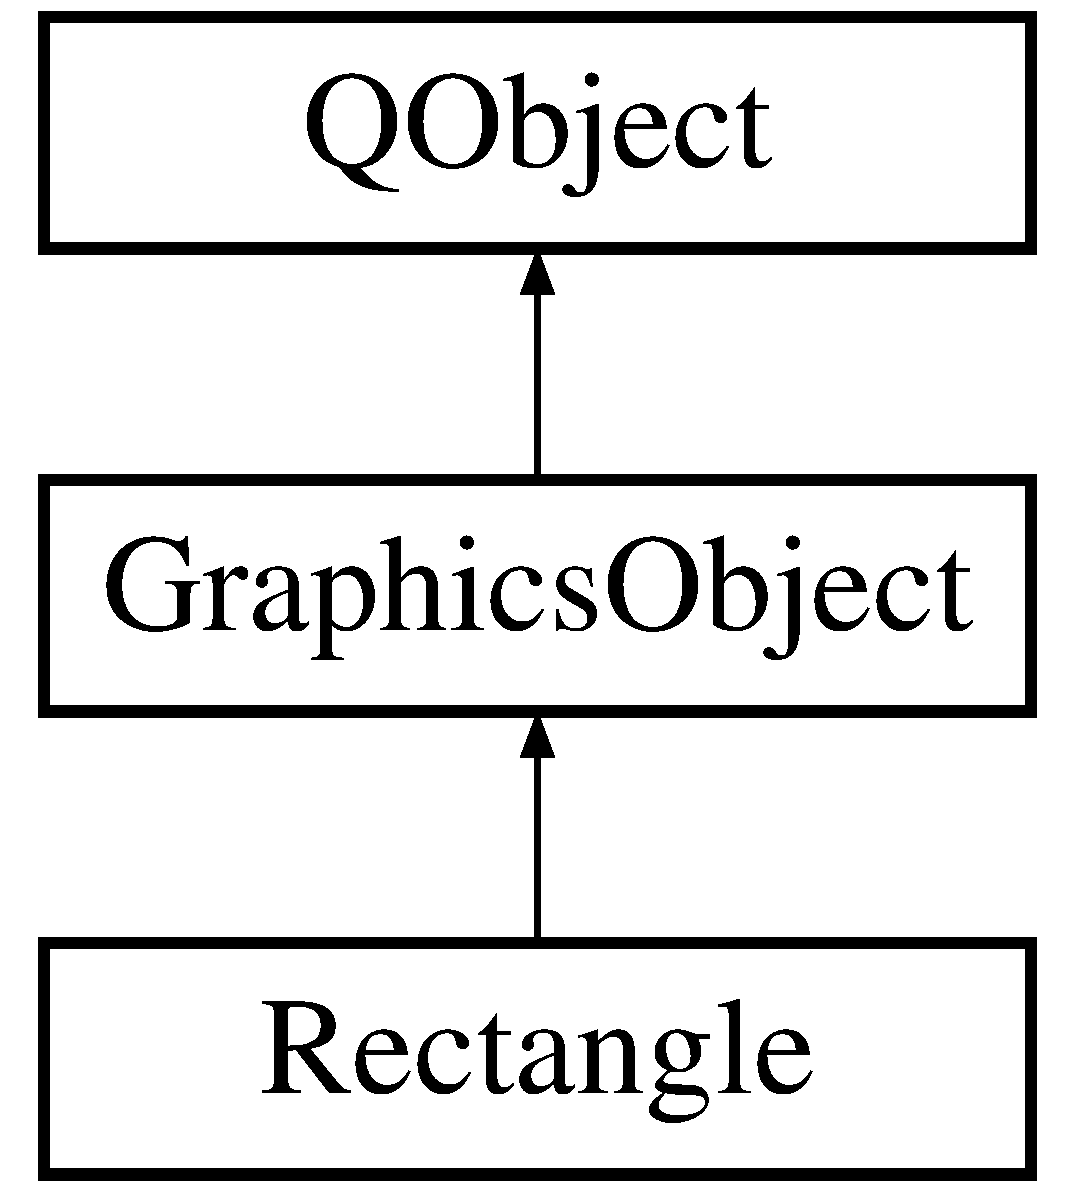
\includegraphics[height=3.000000cm]{class_rectangle}
\end{center}
\end{figure}
\subsection*{Public Member Functions}
\begin{DoxyCompactItemize}
\item 
\hyperlink{class_rectangle_a3a431eeb9b63f2108f171416b205f302}{Rectangle} (Q\+Object $\ast$parent=nullptr)
\begin{DoxyCompactList}\small\item\em \hyperlink{class_rectangle}{Rectangle} Kontruktor wid so geändert dass ein Q\+Object $\ast$parent -\/ Parameter erwartet wird. \end{DoxyCompactList}\item 
\hyperlink{class_rectangle_a07eb215e78b898b77cb843ceb497b46a}{Rectangle} (qreal xkoord, qreal ykoord, qreal width, qreal height, Q\+Color fill, Q\+Color border)
\begin{DoxyCompactList}\small\item\em \hyperlink{class_rectangle}{Rectangle} Konstruktor. \end{DoxyCompactList}\item 
\hyperlink{class_rectangle_a494c076b13aadf26efdce07d23c61ddd}{$\sim$\+Rectangle} ()
\begin{DoxyCompactList}\small\item\em \hyperlink{class_rectangle}{Rectangle} Destruktor. \end{DoxyCompactList}\item 
virtual Q\+Abstract\+Graphics\+Shape\+Item $\ast$ \hyperlink{class_rectangle_aeafbe16d72e37bb155c78a122408d3dc}{graphic\+Shape\+Item} () const
\begin{DoxyCompactList}\small\item\em graphic\+Shape\+Item \end{DoxyCompactList}\item 
virtual Q\+String \hyperlink{class_rectangle_a75b1e77ef828ff8de86cfcf6b03bfadb}{to\+String} ()
\begin{DoxyCompactList}\small\item\em to\+String \end{DoxyCompactList}\end{DoxyCompactItemize}
\subsection*{Protected Attributes}
\begin{DoxyCompactItemize}
\item 
Q\+Graphics\+Rect\+Item $\ast$ \hyperlink{class_rectangle_a4d7f03c65f5e27a63a3299aac6da3954}{m\+\_\+graphics\+Rect}
\end{DoxyCompactItemize}
\subsection*{Static Protected Attributes}
\begin{DoxyCompactItemize}
\item 
static unsigned long \hyperlink{class_rectangle_aa5a0b5d899df185e221e17d032472352}{m\+\_\+rectangle\+Counter} = 0
\end{DoxyCompactItemize}


\subsection{Detailed Description}
The \hyperlink{class_rectangle}{Rectangle} class -\/ Klasse für das Rechteck Objekt abgeleitet von Graphic Objekt. 

\subsection{Constructor \& Destructor Documentation}
\mbox{\Hypertarget{class_rectangle_a3a431eeb9b63f2108f171416b205f302}\label{class_rectangle_a3a431eeb9b63f2108f171416b205f302}} 
\index{Rectangle@{Rectangle}!Rectangle@{Rectangle}}
\index{Rectangle@{Rectangle}!Rectangle@{Rectangle}}
\subsubsection{\texorpdfstring{Rectangle()}{Rectangle()}\hspace{0.1cm}{\footnotesize\ttfamily [1/2]}}
{\footnotesize\ttfamily Rectangle\+::\+Rectangle (\begin{DoxyParamCaption}\item[{Q\+Object $\ast$}]{parent = {\ttfamily nullptr} }\end{DoxyParamCaption})}



\hyperlink{class_rectangle}{Rectangle} Kontruktor wid so geändert dass ein Q\+Object $\ast$parent -\/ Parameter erwartet wird. 

Konstruktor vom Objekt \hyperlink{class_rectangle}{Rectangle}.


\begin{DoxyParams}{Parameters}
{\em parent} & \\
\hline
\end{DoxyParams}
\mbox{\Hypertarget{class_rectangle_a07eb215e78b898b77cb843ceb497b46a}\label{class_rectangle_a07eb215e78b898b77cb843ceb497b46a}} 
\index{Rectangle@{Rectangle}!Rectangle@{Rectangle}}
\index{Rectangle@{Rectangle}!Rectangle@{Rectangle}}
\subsubsection{\texorpdfstring{Rectangle()}{Rectangle()}\hspace{0.1cm}{\footnotesize\ttfamily [2/2]}}
{\footnotesize\ttfamily Rectangle\+::\+Rectangle (\begin{DoxyParamCaption}\item[{qreal}]{xkoord,  }\item[{qreal}]{ykoord,  }\item[{qreal}]{width,  }\item[{qreal}]{height,  }\item[{Q\+Color}]{fill,  }\item[{Q\+Color}]{border }\end{DoxyParamCaption})}



\hyperlink{class_rectangle}{Rectangle} Konstruktor. 

Dieser Konstruktor ist dafür gemacht, um ein aus den übergebenen Werten ein Q\+Graphic\+Rect\+Item zu machen.


\begin{DoxyParams}{Parameters}
{\em position} & \\
\hline
{\em dimension} & \\
\hline
{\em fill} & \\
\hline
{\em border} & \\
\hline
{\em xkoord} & \\
\hline
{\em ykoord} & \\
\hline
{\em width} & \\
\hline
{\em height} & \\
\hline
{\em fill} & \\
\hline
{\em border} & \\
\hline
\end{DoxyParams}
\mbox{\Hypertarget{class_rectangle_a494c076b13aadf26efdce07d23c61ddd}\label{class_rectangle_a494c076b13aadf26efdce07d23c61ddd}} 
\index{Rectangle@{Rectangle}!````~Rectangle@{$\sim$\+Rectangle}}
\index{````~Rectangle@{$\sim$\+Rectangle}!Rectangle@{Rectangle}}
\subsubsection{\texorpdfstring{$\sim$\+Rectangle()}{~Rectangle()}}
{\footnotesize\ttfamily Rectangle\+::$\sim$\+Rectangle (\begin{DoxyParamCaption}{ }\end{DoxyParamCaption})}



\hyperlink{class_rectangle}{Rectangle} Destruktor. 

Destruktor vom Objekt \hyperlink{class_rectangle}{Rectangle}. 

\subsection{Member Function Documentation}
\mbox{\Hypertarget{class_rectangle_aeafbe16d72e37bb155c78a122408d3dc}\label{class_rectangle_aeafbe16d72e37bb155c78a122408d3dc}} 
\index{Rectangle@{Rectangle}!graphic\+Shape\+Item@{graphic\+Shape\+Item}}
\index{graphic\+Shape\+Item@{graphic\+Shape\+Item}!Rectangle@{Rectangle}}
\subsubsection{\texorpdfstring{graphic\+Shape\+Item()}{graphicShapeItem()}}
{\footnotesize\ttfamily Q\+Abstract\+Graphics\+Shape\+Item $\ast$ Rectangle\+::graphic\+Shape\+Item (\begin{DoxyParamCaption}{ }\end{DoxyParamCaption}) const\hspace{0.3cm}{\ttfamily [virtual]}}



graphic\+Shape\+Item 

virtuelle Methode, um das Q\+Graphic\+Rect\+Item wiederzugeben.

\begin{DoxyReturn}{Returns}


m\+\_\+graphics\+Rect 
\end{DoxyReturn}


Reimplemented from \hyperlink{class_graphics_object_ad898be2fdbcc4c57f908cdd6a3feaa44}{Graphics\+Object}.

\mbox{\Hypertarget{class_rectangle_a75b1e77ef828ff8de86cfcf6b03bfadb}\label{class_rectangle_a75b1e77ef828ff8de86cfcf6b03bfadb}} 
\index{Rectangle@{Rectangle}!to\+String@{to\+String}}
\index{to\+String@{to\+String}!Rectangle@{Rectangle}}
\subsubsection{\texorpdfstring{to\+String()}{toString()}}
{\footnotesize\ttfamily Q\+String Rectangle\+::to\+String (\begin{DoxyParamCaption}{ }\end{DoxyParamCaption})\hspace{0.3cm}{\ttfamily [virtual]}}



to\+String 

\hyperlink{class_rectangle_a75b1e77ef828ff8de86cfcf6b03bfadb}{Rectangle\+::to\+String} -\/ Methode, gibt alle Eigenschaften des Rechtecks aus.

\begin{DoxyReturn}{Returns}

\end{DoxyReturn}


Reimplemented from \hyperlink{class_graphics_object_ad985316df1516a5a7311161250b5e233}{Graphics\+Object}.



\subsection{Member Data Documentation}
\mbox{\Hypertarget{class_rectangle_a4d7f03c65f5e27a63a3299aac6da3954}\label{class_rectangle_a4d7f03c65f5e27a63a3299aac6da3954}} 
\index{Rectangle@{Rectangle}!m\+\_\+graphics\+Rect@{m\+\_\+graphics\+Rect}}
\index{m\+\_\+graphics\+Rect@{m\+\_\+graphics\+Rect}!Rectangle@{Rectangle}}
\subsubsection{\texorpdfstring{m\+\_\+graphics\+Rect}{m\_graphicsRect}}
{\footnotesize\ttfamily Q\+Graphics\+Rect\+Item$\ast$ Rectangle\+::m\+\_\+graphics\+Rect\hspace{0.3cm}{\ttfamily [protected]}}

\mbox{\Hypertarget{class_rectangle_aa5a0b5d899df185e221e17d032472352}\label{class_rectangle_aa5a0b5d899df185e221e17d032472352}} 
\index{Rectangle@{Rectangle}!m\+\_\+rectangle\+Counter@{m\+\_\+rectangle\+Counter}}
\index{m\+\_\+rectangle\+Counter@{m\+\_\+rectangle\+Counter}!Rectangle@{Rectangle}}
\subsubsection{\texorpdfstring{m\+\_\+rectangle\+Counter}{m\_rectangleCounter}}
{\footnotesize\ttfamily unsigned long Rectangle\+::m\+\_\+rectangle\+Counter = 0\hspace{0.3cm}{\ttfamily [static]}, {\ttfamily [protected]}}



The documentation for this class was generated from the following files\+:\begin{DoxyCompactItemize}
\item 
C\+:/\+Users/tranb/\+Desktop/\+Sciebo/\+Studium/\+Qt Projekte/\+Graphic\+Obj/\hyperlink{rectangle_8h}{rectangle.\+h}\item 
C\+:/\+Users/tranb/\+Desktop/\+Sciebo/\+Studium/\+Qt Projekte/\+Graphic\+Obj/\hyperlink{rectangle_8cpp}{rectangle.\+cpp}\end{DoxyCompactItemize}

\hypertarget{class_tools}{}\section{Tools Class Reference}
\label{class_tools}\index{Tools@{Tools}}


The \hyperlink{class_tools}{Tools} class -\/ Klasse für die Zeichenwerkzeuge und Einstellung von Füllfarbe und Rahmenfarbe.  




{\ttfamily \#include $<$tools.\+h$>$}

Inheritance diagram for Tools\+:\begin{figure}[H]
\begin{center}
\leavevmode
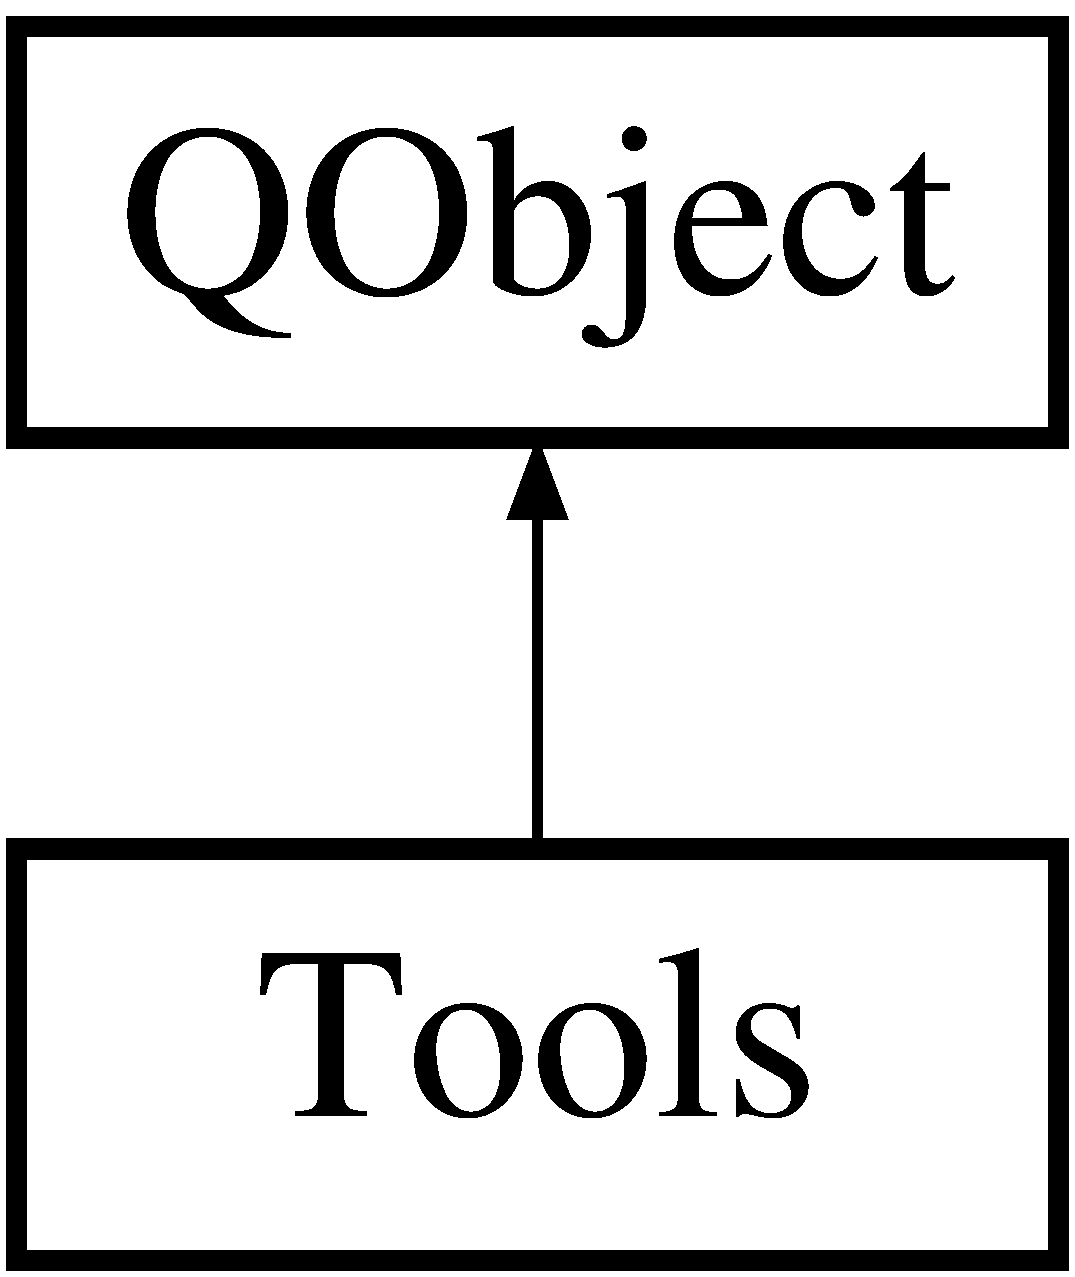
\includegraphics[height=2.000000cm]{class_tools}
\end{center}
\end{figure}
\subsection*{Public Types}
\begin{DoxyCompactItemize}
\item 
enum \hyperlink{class_tools_a2847c269682818722541d9002fdf0824}{State} \{ \hyperlink{class_tools_a2847c269682818722541d9002fdf0824a39a562c65ff6fde1589fd79d63b16b31}{N\+O\+N\+E\+\_\+\+A\+C\+T\+I\+VE}, 
\hyperlink{class_tools_a2847c269682818722541d9002fdf0824ad6c9098c08b610749e430f97f83f95bd}{G\+R\+A\+B\+B\+E\+R\+\_\+\+A\+C\+T\+I\+VE}, 
\hyperlink{class_tools_a2847c269682818722541d9002fdf0824a19672b3e28d4946b8edd3b42bd20508a}{R\+E\+C\+T\+\_\+\+A\+C\+T\+I\+VE}, 
\hyperlink{class_tools_a2847c269682818722541d9002fdf0824af205a7ab0929002ae4bec7fae92a31e1}{C\+I\+R\+C\+\_\+\+A\+C\+T\+I\+VE}
 \}\begin{DoxyCompactList}\small\item\em The State enum. \end{DoxyCompactList}
\item 
enum \hyperlink{class_tools_ab031688a77e89a80ce8b5db7014684a3}{Draw\+Tool} \{ \hyperlink{class_tools_ab031688a77e89a80ce8b5db7014684a3a563beaca84fc18e79f568499ee8fdee7}{G\+R\+A\+B\+B\+ER}, 
\hyperlink{class_tools_ab031688a77e89a80ce8b5db7014684a3a7608a149cc544834de7d2274fa175237}{C\+I\+R\+C\+LE}, 
\hyperlink{class_tools_ab031688a77e89a80ce8b5db7014684a3abc11dd73d5c7e1996dbcf0aab00d095b}{R\+E\+C\+T\+A\+N\+G\+LE}, 
\hyperlink{class_tools_ab031688a77e89a80ce8b5db7014684a3a883ff4bc5dc9f42f40f091328bcf1907}{P\+O\+L\+Y\+G\+ON}
 \}\begin{DoxyCompactList}\small\item\em The Draw\+Tool enum. \end{DoxyCompactList}
\item 
enum \hyperlink{class_tools_a4b55b2ca4eef4d80ae1042233832bb8b}{Option\+Tool} \{ \hyperlink{class_tools_a4b55b2ca4eef4d80ae1042233832bb8ba670c67a855fba32a19f09a8e794d1b8e}{G\+R\+U\+N\+D\+R\+I\+SS}, 
\hyperlink{class_tools_a4b55b2ca4eef4d80ae1042233832bb8ba53d0273a369699f49786930287a5e675}{M\+O\+E\+B\+EL}
 \}\begin{DoxyCompactList}\small\item\em The Option\+Tool enum. \end{DoxyCompactList}
\end{DoxyCompactItemize}
\subsection*{Public Slots}
\begin{DoxyCompactItemize}
\item 
void \hyperlink{class_tools_a4912994771a4424b9aec1a7b16d31176}{set\+Fill\+Color} (const Q\+Color \&value)
\begin{DoxyCompactList}\small\item\em set\+Fill\+Color -\/ Setter Methode für Füllfarbe \end{DoxyCompactList}\item 
void \hyperlink{class_tools_a94304e05407643ce69f20ba93538d3d5}{set\+Border\+Color} (const Q\+Color \&value)
\begin{DoxyCompactList}\small\item\em set\+Border\+Color -\/ Setter Methode für Rahmenfarbe \end{DoxyCompactList}\item 
void \hyperlink{class_tools_abdf68db9740ba504701fe00d97a031e2}{set\+State} (\hyperlink{class_tools_a2847c269682818722541d9002fdf0824}{State} state)
\begin{DoxyCompactList}\small\item\em set\+State -\/ Setter Methode für State \end{DoxyCompactList}\item 
void \hyperlink{class_tools_aa53c7186fb6cd6104ff42014b6f44f93}{set\+Draw\+Tool} (const \hyperlink{class_tools_ab031688a77e89a80ce8b5db7014684a3}{Tools\+::\+Draw\+Tool} drawtool)
\begin{DoxyCompactList}\small\item\em set\+Draw\+Tool -\/ Setter Methode für das Auswahlwerkzeug \end{DoxyCompactList}\item 
void \hyperlink{class_tools_af69d4aa896ef3e1b06ce65e5df53f060}{set\+Option\+Tool} (const \hyperlink{class_tools_a4b55b2ca4eef4d80ae1042233832bb8b}{Tools\+::\+Option\+Tool} option\+Tool)
\begin{DoxyCompactList}\small\item\em set\+Option\+Tool -\/ Setter Methode für das Option\+Tool Werkzeug. \end{DoxyCompactList}\end{DoxyCompactItemize}
\subsection*{Signals}
\begin{DoxyCompactItemize}
\item 
void \hyperlink{class_tools_ab5d002810a63050d8a7fd2e1b19b2ba0}{active\+Draw\+Tool\+Changed} (const \hyperlink{class_tools_ab031688a77e89a80ce8b5db7014684a3}{Tools\+::\+Draw\+Tool} \&value)
\begin{DoxyCompactList}\small\item\em active\+Draw\+Tool\+Changed -\/ Signal, das aussendet wenn ein Auswahlwerkzeug geändert wurde. \end{DoxyCompactList}\item 
void \hyperlink{class_tools_a3feb94811769e2b47a1e9ad543bda1f8}{active\+Border\+Color\+Changed} (Q\+Color color)
\begin{DoxyCompactList}\small\item\em active\+Border\+Color\+Changed -\/ Signal, das aussendet wenn die Rahmenfarbe geändert wurde \end{DoxyCompactList}\item 
void \hyperlink{class_tools_a1330acf72b4e751cb873d6538cc5ef2d}{active\+Fill\+Color\+Changed} (Q\+Color color)
\begin{DoxyCompactList}\small\item\em active\+Fill\+Color\+Changed -\/\+Signal, das aussendet wenn die Füllfarbe geänert wurde \end{DoxyCompactList}\item 
void \hyperlink{class_tools_a6ea189495868e06c89d79b36d09b43d7}{active\+Option\+Tool\+Changed} (const \hyperlink{class_tools_a4b55b2ca4eef4d80ae1042233832bb8b}{Tools\+::\+Option\+Tool} \&value)
\begin{DoxyCompactList}\small\item\em active\+Option\+Tool\+Changed -\/ Getter -\/ Methode für das Option\+Tool Werkzeug. \end{DoxyCompactList}\end{DoxyCompactItemize}
\subsection*{Public Member Functions}
\begin{DoxyCompactItemize}
\item 
\hyperlink{class_tools_a33adedcb5a43ffd5a1b62515b4a3db2c}{Tools} (Q\+Object $\ast$parent=nullptr)
\begin{DoxyCompactList}\small\item\em \hyperlink{class_tools_a33adedcb5a43ffd5a1b62515b4a3db2c}{Tools\+::\+Tools} Konstruktor. \end{DoxyCompactList}\item 
Q\+Color \hyperlink{class_tools_a263df3826bfd5975d1e379060ea554dc}{get\+Border\+Color} () const
\begin{DoxyCompactList}\small\item\em Getter -\/ Methode für Border\+Color. \end{DoxyCompactList}\item 
Q\+Color \hyperlink{class_tools_acb1e17bcb34c9290423b55a7f92d9936}{get\+Fill\+Color} () const
\begin{DoxyCompactList}\small\item\em Getter -\/ Methode für Fill\+Color. \end{DoxyCompactList}\item 
\hyperlink{class_tools_a2847c269682818722541d9002fdf0824}{State} \hyperlink{class_tools_ae81ec47ff47279c8a8f319d822c3bb9f}{get\+State} ()
\begin{DoxyCompactList}\small\item\em get\+State \end{DoxyCompactList}\item 
\hyperlink{class_tools_ab031688a77e89a80ce8b5db7014684a3}{Draw\+Tool} \hyperlink{class_tools_a4e8bdc1c74c1d9b5969c6b8afef0f805}{get\+Draw\+Tool} ()
\begin{DoxyCompactList}\small\item\em get\+Draw\+Tool -\/ Setter Methode für das Auswahlwerkzeug \end{DoxyCompactList}\item 
\hyperlink{class_tools_a4b55b2ca4eef4d80ae1042233832bb8b}{Option\+Tool} \hyperlink{class_tools_a45d1e69e6f93c92df35756f3b48092ca}{get\+Option\+Tool} ()
\begin{DoxyCompactList}\small\item\em \hyperlink{class_tools_a45d1e69e6f93c92df35756f3b48092ca}{Tools\+::get\+Option\+Tool} -\/ Getter -\/ Methode, welche das Optionwerkzeug zurückgibt. (Grundriss oder Moebel) \end{DoxyCompactList}\end{DoxyCompactItemize}
\subsection*{Protected Attributes}
\begin{DoxyCompactItemize}
\item 
\hyperlink{class_tools_ab031688a77e89a80ce8b5db7014684a3}{Tools\+::\+Draw\+Tool} \hyperlink{class_tools_a8777299234b214fb917f42c0ef1a0ead}{werkzeug}
\item 
\hyperlink{class_tools_a4b55b2ca4eef4d80ae1042233832bb8b}{Tools\+::\+Option\+Tool} \hyperlink{class_tools_a9bf140c9c0af40044aaa2c115b632399}{option}
\item 
\hyperlink{class_tools_a2847c269682818722541d9002fdf0824}{State} \hyperlink{class_tools_a9ee6b69697a16133db9d1f24346cd838}{status}
\item 
Q\+Color \hyperlink{class_tools_af7de157c4f6575664512accd32d93a43}{border\+Color}
\item 
Q\+Color \hyperlink{class_tools_a522e6149eb1349df97fa1bb7abaec427}{fill\+Color}
\end{DoxyCompactItemize}


\subsection{Detailed Description}
The \hyperlink{class_tools}{Tools} class -\/ Klasse für die Zeichenwerkzeuge und Einstellung von Füllfarbe und Rahmenfarbe. 

\subsection{Member Enumeration Documentation}
\mbox{\Hypertarget{class_tools_ab031688a77e89a80ce8b5db7014684a3}\label{class_tools_ab031688a77e89a80ce8b5db7014684a3}} 
\index{Tools@{Tools}!Draw\+Tool@{Draw\+Tool}}
\index{Draw\+Tool@{Draw\+Tool}!Tools@{Tools}}
\subsubsection{\texorpdfstring{Draw\+Tool}{DrawTool}}
{\footnotesize\ttfamily enum \hyperlink{class_tools_ab031688a77e89a80ce8b5db7014684a3}{Tools\+::\+Draw\+Tool}}



The Draw\+Tool enum. 

\begin{DoxyEnumFields}{Enumerator}
\raisebox{\heightof{T}}[0pt][0pt]{\index{G\+R\+A\+B\+B\+ER@{G\+R\+A\+B\+B\+ER}!Tools@{Tools}}\index{Tools@{Tools}!G\+R\+A\+B\+B\+ER@{G\+R\+A\+B\+B\+ER}}}\mbox{\Hypertarget{class_tools_ab031688a77e89a80ce8b5db7014684a3a563beaca84fc18e79f568499ee8fdee7}\label{class_tools_ab031688a77e89a80ce8b5db7014684a3a563beaca84fc18e79f568499ee8fdee7}} 
G\+R\+A\+B\+B\+ER&\\
\hline

\raisebox{\heightof{T}}[0pt][0pt]{\index{C\+I\+R\+C\+LE@{C\+I\+R\+C\+LE}!Tools@{Tools}}\index{Tools@{Tools}!C\+I\+R\+C\+LE@{C\+I\+R\+C\+LE}}}\mbox{\Hypertarget{class_tools_ab031688a77e89a80ce8b5db7014684a3a7608a149cc544834de7d2274fa175237}\label{class_tools_ab031688a77e89a80ce8b5db7014684a3a7608a149cc544834de7d2274fa175237}} 
C\+I\+R\+C\+LE&\\
\hline

\raisebox{\heightof{T}}[0pt][0pt]{\index{R\+E\+C\+T\+A\+N\+G\+LE@{R\+E\+C\+T\+A\+N\+G\+LE}!Tools@{Tools}}\index{Tools@{Tools}!R\+E\+C\+T\+A\+N\+G\+LE@{R\+E\+C\+T\+A\+N\+G\+LE}}}\mbox{\Hypertarget{class_tools_ab031688a77e89a80ce8b5db7014684a3abc11dd73d5c7e1996dbcf0aab00d095b}\label{class_tools_ab031688a77e89a80ce8b5db7014684a3abc11dd73d5c7e1996dbcf0aab00d095b}} 
R\+E\+C\+T\+A\+N\+G\+LE&\\
\hline

\raisebox{\heightof{T}}[0pt][0pt]{\index{P\+O\+L\+Y\+G\+ON@{P\+O\+L\+Y\+G\+ON}!Tools@{Tools}}\index{Tools@{Tools}!P\+O\+L\+Y\+G\+ON@{P\+O\+L\+Y\+G\+ON}}}\mbox{\Hypertarget{class_tools_ab031688a77e89a80ce8b5db7014684a3a883ff4bc5dc9f42f40f091328bcf1907}\label{class_tools_ab031688a77e89a80ce8b5db7014684a3a883ff4bc5dc9f42f40f091328bcf1907}} 
P\+O\+L\+Y\+G\+ON&\\
\hline

\end{DoxyEnumFields}
\mbox{\Hypertarget{class_tools_a4b55b2ca4eef4d80ae1042233832bb8b}\label{class_tools_a4b55b2ca4eef4d80ae1042233832bb8b}} 
\index{Tools@{Tools}!Option\+Tool@{Option\+Tool}}
\index{Option\+Tool@{Option\+Tool}!Tools@{Tools}}
\subsubsection{\texorpdfstring{Option\+Tool}{OptionTool}}
{\footnotesize\ttfamily enum \hyperlink{class_tools_a4b55b2ca4eef4d80ae1042233832bb8b}{Tools\+::\+Option\+Tool}}



The Option\+Tool enum. 

\begin{DoxyEnumFields}{Enumerator}
\raisebox{\heightof{T}}[0pt][0pt]{\index{G\+R\+U\+N\+D\+R\+I\+SS@{G\+R\+U\+N\+D\+R\+I\+SS}!Tools@{Tools}}\index{Tools@{Tools}!G\+R\+U\+N\+D\+R\+I\+SS@{G\+R\+U\+N\+D\+R\+I\+SS}}}\mbox{\Hypertarget{class_tools_a4b55b2ca4eef4d80ae1042233832bb8ba670c67a855fba32a19f09a8e794d1b8e}\label{class_tools_a4b55b2ca4eef4d80ae1042233832bb8ba670c67a855fba32a19f09a8e794d1b8e}} 
G\+R\+U\+N\+D\+R\+I\+SS&\\
\hline

\raisebox{\heightof{T}}[0pt][0pt]{\index{M\+O\+E\+B\+EL@{M\+O\+E\+B\+EL}!Tools@{Tools}}\index{Tools@{Tools}!M\+O\+E\+B\+EL@{M\+O\+E\+B\+EL}}}\mbox{\Hypertarget{class_tools_a4b55b2ca4eef4d80ae1042233832bb8ba53d0273a369699f49786930287a5e675}\label{class_tools_a4b55b2ca4eef4d80ae1042233832bb8ba53d0273a369699f49786930287a5e675}} 
M\+O\+E\+B\+EL&\\
\hline

\end{DoxyEnumFields}
\mbox{\Hypertarget{class_tools_a2847c269682818722541d9002fdf0824}\label{class_tools_a2847c269682818722541d9002fdf0824}} 
\index{Tools@{Tools}!State@{State}}
\index{State@{State}!Tools@{Tools}}
\subsubsection{\texorpdfstring{State}{State}}
{\footnotesize\ttfamily enum \hyperlink{class_tools_a2847c269682818722541d9002fdf0824}{Tools\+::\+State}}



The State enum. 

\begin{DoxyEnumFields}{Enumerator}
\raisebox{\heightof{T}}[0pt][0pt]{\index{N\+O\+N\+E\+\_\+\+A\+C\+T\+I\+VE@{N\+O\+N\+E\+\_\+\+A\+C\+T\+I\+VE}!Tools@{Tools}}\index{Tools@{Tools}!N\+O\+N\+E\+\_\+\+A\+C\+T\+I\+VE@{N\+O\+N\+E\+\_\+\+A\+C\+T\+I\+VE}}}\mbox{\Hypertarget{class_tools_a2847c269682818722541d9002fdf0824a39a562c65ff6fde1589fd79d63b16b31}\label{class_tools_a2847c269682818722541d9002fdf0824a39a562c65ff6fde1589fd79d63b16b31}} 
N\+O\+N\+E\+\_\+\+A\+C\+T\+I\+VE&\\
\hline

\raisebox{\heightof{T}}[0pt][0pt]{\index{G\+R\+A\+B\+B\+E\+R\+\_\+\+A\+C\+T\+I\+VE@{G\+R\+A\+B\+B\+E\+R\+\_\+\+A\+C\+T\+I\+VE}!Tools@{Tools}}\index{Tools@{Tools}!G\+R\+A\+B\+B\+E\+R\+\_\+\+A\+C\+T\+I\+VE@{G\+R\+A\+B\+B\+E\+R\+\_\+\+A\+C\+T\+I\+VE}}}\mbox{\Hypertarget{class_tools_a2847c269682818722541d9002fdf0824ad6c9098c08b610749e430f97f83f95bd}\label{class_tools_a2847c269682818722541d9002fdf0824ad6c9098c08b610749e430f97f83f95bd}} 
G\+R\+A\+B\+B\+E\+R\+\_\+\+A\+C\+T\+I\+VE&\\
\hline

\raisebox{\heightof{T}}[0pt][0pt]{\index{R\+E\+C\+T\+\_\+\+A\+C\+T\+I\+VE@{R\+E\+C\+T\+\_\+\+A\+C\+T\+I\+VE}!Tools@{Tools}}\index{Tools@{Tools}!R\+E\+C\+T\+\_\+\+A\+C\+T\+I\+VE@{R\+E\+C\+T\+\_\+\+A\+C\+T\+I\+VE}}}\mbox{\Hypertarget{class_tools_a2847c269682818722541d9002fdf0824a19672b3e28d4946b8edd3b42bd20508a}\label{class_tools_a2847c269682818722541d9002fdf0824a19672b3e28d4946b8edd3b42bd20508a}} 
R\+E\+C\+T\+\_\+\+A\+C\+T\+I\+VE&\\
\hline

\raisebox{\heightof{T}}[0pt][0pt]{\index{C\+I\+R\+C\+\_\+\+A\+C\+T\+I\+VE@{C\+I\+R\+C\+\_\+\+A\+C\+T\+I\+VE}!Tools@{Tools}}\index{Tools@{Tools}!C\+I\+R\+C\+\_\+\+A\+C\+T\+I\+VE@{C\+I\+R\+C\+\_\+\+A\+C\+T\+I\+VE}}}\mbox{\Hypertarget{class_tools_a2847c269682818722541d9002fdf0824af205a7ab0929002ae4bec7fae92a31e1}\label{class_tools_a2847c269682818722541d9002fdf0824af205a7ab0929002ae4bec7fae92a31e1}} 
C\+I\+R\+C\+\_\+\+A\+C\+T\+I\+VE&\\
\hline

\end{DoxyEnumFields}


\subsection{Constructor \& Destructor Documentation}
\mbox{\Hypertarget{class_tools_a33adedcb5a43ffd5a1b62515b4a3db2c}\label{class_tools_a33adedcb5a43ffd5a1b62515b4a3db2c}} 
\index{Tools@{Tools}!Tools@{Tools}}
\index{Tools@{Tools}!Tools@{Tools}}
\subsubsection{\texorpdfstring{Tools()}{Tools()}}
{\footnotesize\ttfamily Tools\+::\+Tools (\begin{DoxyParamCaption}\item[{Q\+Object $\ast$}]{parent = {\ttfamily nullptr} }\end{DoxyParamCaption})\hspace{0.3cm}{\ttfamily [explicit]}}



\hyperlink{class_tools_a33adedcb5a43ffd5a1b62515b4a3db2c}{Tools\+::\+Tools} Konstruktor. 


\begin{DoxyParams}{Parameters}
{\em parent} & \\
\hline
\end{DoxyParams}


\subsection{Member Function Documentation}
\mbox{\Hypertarget{class_tools_a3feb94811769e2b47a1e9ad543bda1f8}\label{class_tools_a3feb94811769e2b47a1e9ad543bda1f8}} 
\index{Tools@{Tools}!active\+Border\+Color\+Changed@{active\+Border\+Color\+Changed}}
\index{active\+Border\+Color\+Changed@{active\+Border\+Color\+Changed}!Tools@{Tools}}
\subsubsection{\texorpdfstring{active\+Border\+Color\+Changed}{activeBorderColorChanged}}
{\footnotesize\ttfamily void Tools\+::active\+Border\+Color\+Changed (\begin{DoxyParamCaption}\item[{Q\+Color}]{color }\end{DoxyParamCaption})\hspace{0.3cm}{\ttfamily [signal]}}



active\+Border\+Color\+Changed -\/ Signal, das aussendet wenn die Rahmenfarbe geändert wurde 


\begin{DoxyParams}{Parameters}
{\em color} & \\
\hline
\end{DoxyParams}
\mbox{\Hypertarget{class_tools_ab5d002810a63050d8a7fd2e1b19b2ba0}\label{class_tools_ab5d002810a63050d8a7fd2e1b19b2ba0}} 
\index{Tools@{Tools}!active\+Draw\+Tool\+Changed@{active\+Draw\+Tool\+Changed}}
\index{active\+Draw\+Tool\+Changed@{active\+Draw\+Tool\+Changed}!Tools@{Tools}}
\subsubsection{\texorpdfstring{active\+Draw\+Tool\+Changed}{activeDrawToolChanged}}
{\footnotesize\ttfamily void Tools\+::active\+Draw\+Tool\+Changed (\begin{DoxyParamCaption}\item[{const \hyperlink{class_tools_ab031688a77e89a80ce8b5db7014684a3}{Tools\+::\+Draw\+Tool} \&}]{value }\end{DoxyParamCaption})\hspace{0.3cm}{\ttfamily [signal]}}



active\+Draw\+Tool\+Changed -\/ Signal, das aussendet wenn ein Auswahlwerkzeug geändert wurde. 


\begin{DoxyParams}{Parameters}
{\em value} & \\
\hline
\end{DoxyParams}
\mbox{\Hypertarget{class_tools_a1330acf72b4e751cb873d6538cc5ef2d}\label{class_tools_a1330acf72b4e751cb873d6538cc5ef2d}} 
\index{Tools@{Tools}!active\+Fill\+Color\+Changed@{active\+Fill\+Color\+Changed}}
\index{active\+Fill\+Color\+Changed@{active\+Fill\+Color\+Changed}!Tools@{Tools}}
\subsubsection{\texorpdfstring{active\+Fill\+Color\+Changed}{activeFillColorChanged}}
{\footnotesize\ttfamily void Tools\+::active\+Fill\+Color\+Changed (\begin{DoxyParamCaption}\item[{Q\+Color}]{color }\end{DoxyParamCaption})\hspace{0.3cm}{\ttfamily [signal]}}



active\+Fill\+Color\+Changed -\/\+Signal, das aussendet wenn die Füllfarbe geänert wurde 


\begin{DoxyParams}{Parameters}
{\em color} & \\
\hline
\end{DoxyParams}
\mbox{\Hypertarget{class_tools_a6ea189495868e06c89d79b36d09b43d7}\label{class_tools_a6ea189495868e06c89d79b36d09b43d7}} 
\index{Tools@{Tools}!active\+Option\+Tool\+Changed@{active\+Option\+Tool\+Changed}}
\index{active\+Option\+Tool\+Changed@{active\+Option\+Tool\+Changed}!Tools@{Tools}}
\subsubsection{\texorpdfstring{active\+Option\+Tool\+Changed}{activeOptionToolChanged}}
{\footnotesize\ttfamily void Tools\+::active\+Option\+Tool\+Changed (\begin{DoxyParamCaption}\item[{const \hyperlink{class_tools_a4b55b2ca4eef4d80ae1042233832bb8b}{Tools\+::\+Option\+Tool} \&}]{value }\end{DoxyParamCaption})\hspace{0.3cm}{\ttfamily [signal]}}



active\+Option\+Tool\+Changed -\/ Getter -\/ Methode für das Option\+Tool Werkzeug. 


\begin{DoxyParams}{Parameters}
{\em value} & \\
\hline
\end{DoxyParams}
\mbox{\Hypertarget{class_tools_a263df3826bfd5975d1e379060ea554dc}\label{class_tools_a263df3826bfd5975d1e379060ea554dc}} 
\index{Tools@{Tools}!get\+Border\+Color@{get\+Border\+Color}}
\index{get\+Border\+Color@{get\+Border\+Color}!Tools@{Tools}}
\subsubsection{\texorpdfstring{get\+Border\+Color()}{getBorderColor()}}
{\footnotesize\ttfamily Q\+Color Tools\+::get\+Border\+Color (\begin{DoxyParamCaption}{ }\end{DoxyParamCaption}) const}



Getter -\/ Methode für Border\+Color. 

\hyperlink{class_tools_a263df3826bfd5975d1e379060ea554dc}{Tools\+::get\+Border\+Color}.

\begin{DoxyReturn}{Returns}
border\+Color 
\end{DoxyReturn}
\mbox{\Hypertarget{class_tools_a4e8bdc1c74c1d9b5969c6b8afef0f805}\label{class_tools_a4e8bdc1c74c1d9b5969c6b8afef0f805}} 
\index{Tools@{Tools}!get\+Draw\+Tool@{get\+Draw\+Tool}}
\index{get\+Draw\+Tool@{get\+Draw\+Tool}!Tools@{Tools}}
\subsubsection{\texorpdfstring{get\+Draw\+Tool()}{getDrawTool()}}
{\footnotesize\ttfamily \hyperlink{class_tools_ab031688a77e89a80ce8b5db7014684a3}{Tools\+::\+Draw\+Tool} Tools\+::get\+Draw\+Tool (\begin{DoxyParamCaption}{ }\end{DoxyParamCaption})}



get\+Draw\+Tool -\/ Setter Methode für das Auswahlwerkzeug 

\hyperlink{class_tools_a4e8bdc1c74c1d9b5969c6b8afef0f805}{Tools\+::get\+Draw\+Tool} -\/ Getter -\/ Methode, welche das Zeichenwerkzeug zurückgibt.

\begin{DoxyReturn}{Returns}


werkzeug 
\end{DoxyReturn}
\mbox{\Hypertarget{class_tools_acb1e17bcb34c9290423b55a7f92d9936}\label{class_tools_acb1e17bcb34c9290423b55a7f92d9936}} 
\index{Tools@{Tools}!get\+Fill\+Color@{get\+Fill\+Color}}
\index{get\+Fill\+Color@{get\+Fill\+Color}!Tools@{Tools}}
\subsubsection{\texorpdfstring{get\+Fill\+Color()}{getFillColor()}}
{\footnotesize\ttfamily Q\+Color Tools\+::get\+Fill\+Color (\begin{DoxyParamCaption}{ }\end{DoxyParamCaption}) const}



Getter -\/ Methode für Fill\+Color. 

\hyperlink{class_tools_acb1e17bcb34c9290423b55a7f92d9936}{Tools\+::get\+Fill\+Color}.

\begin{DoxyReturn}{Returns}
fill\+Color 
\end{DoxyReturn}
\mbox{\Hypertarget{class_tools_a45d1e69e6f93c92df35756f3b48092ca}\label{class_tools_a45d1e69e6f93c92df35756f3b48092ca}} 
\index{Tools@{Tools}!get\+Option\+Tool@{get\+Option\+Tool}}
\index{get\+Option\+Tool@{get\+Option\+Tool}!Tools@{Tools}}
\subsubsection{\texorpdfstring{get\+Option\+Tool()}{getOptionTool()}}
{\footnotesize\ttfamily \hyperlink{class_tools_a4b55b2ca4eef4d80ae1042233832bb8b}{Tools\+::\+Option\+Tool} Tools\+::get\+Option\+Tool (\begin{DoxyParamCaption}{ }\end{DoxyParamCaption})}



\hyperlink{class_tools_a45d1e69e6f93c92df35756f3b48092ca}{Tools\+::get\+Option\+Tool} -\/ Getter -\/ Methode, welche das Optionwerkzeug zurückgibt. (Grundriss oder Moebel) 

\begin{DoxyReturn}{Returns}
option 
\end{DoxyReturn}
\mbox{\Hypertarget{class_tools_ae81ec47ff47279c8a8f319d822c3bb9f}\label{class_tools_ae81ec47ff47279c8a8f319d822c3bb9f}} 
\index{Tools@{Tools}!get\+State@{get\+State}}
\index{get\+State@{get\+State}!Tools@{Tools}}
\subsubsection{\texorpdfstring{get\+State()}{getState()}}
{\footnotesize\ttfamily \hyperlink{class_tools_a2847c269682818722541d9002fdf0824}{Tools\+::\+State} Tools\+::get\+State (\begin{DoxyParamCaption}{ }\end{DoxyParamCaption})}



get\+State 

\hyperlink{class_tools_ae81ec47ff47279c8a8f319d822c3bb9f}{Tools\+::get\+State}.

\begin{DoxyReturn}{Returns}


status 
\end{DoxyReturn}
\mbox{\Hypertarget{class_tools_a94304e05407643ce69f20ba93538d3d5}\label{class_tools_a94304e05407643ce69f20ba93538d3d5}} 
\index{Tools@{Tools}!set\+Border\+Color@{set\+Border\+Color}}
\index{set\+Border\+Color@{set\+Border\+Color}!Tools@{Tools}}
\subsubsection{\texorpdfstring{set\+Border\+Color}{setBorderColor}}
{\footnotesize\ttfamily void Tools\+::set\+Border\+Color (\begin{DoxyParamCaption}\item[{const Q\+Color \&}]{value }\end{DoxyParamCaption})\hspace{0.3cm}{\ttfamily [slot]}}



set\+Border\+Color -\/ Setter Methode für Rahmenfarbe 

\hyperlink{class_tools_a94304e05407643ce69f20ba93538d3d5}{Tools\+::set\+Border\+Color}.


\begin{DoxyParams}{Parameters}
{\em value} & \\
\hline
\end{DoxyParams}
\mbox{\Hypertarget{class_tools_aa53c7186fb6cd6104ff42014b6f44f93}\label{class_tools_aa53c7186fb6cd6104ff42014b6f44f93}} 
\index{Tools@{Tools}!set\+Draw\+Tool@{set\+Draw\+Tool}}
\index{set\+Draw\+Tool@{set\+Draw\+Tool}!Tools@{Tools}}
\subsubsection{\texorpdfstring{set\+Draw\+Tool}{setDrawTool}}
{\footnotesize\ttfamily void Tools\+::set\+Draw\+Tool (\begin{DoxyParamCaption}\item[{const \hyperlink{class_tools_ab031688a77e89a80ce8b5db7014684a3}{Tools\+::\+Draw\+Tool}}]{drawtool }\end{DoxyParamCaption})\hspace{0.3cm}{\ttfamily [slot]}}



set\+Draw\+Tool -\/ Setter Methode für das Auswahlwerkzeug 

\hyperlink{class_tools_aa53c7186fb6cd6104ff42014b6f44f93}{Tools\+::set\+Draw\+Tool} -\/ Setzt das Zeichenwerkzeug.


\begin{DoxyParams}{Parameters}
{\em drawtool} & \\
\hline
\end{DoxyParams}
\mbox{\Hypertarget{class_tools_a4912994771a4424b9aec1a7b16d31176}\label{class_tools_a4912994771a4424b9aec1a7b16d31176}} 
\index{Tools@{Tools}!set\+Fill\+Color@{set\+Fill\+Color}}
\index{set\+Fill\+Color@{set\+Fill\+Color}!Tools@{Tools}}
\subsubsection{\texorpdfstring{set\+Fill\+Color}{setFillColor}}
{\footnotesize\ttfamily void Tools\+::set\+Fill\+Color (\begin{DoxyParamCaption}\item[{const Q\+Color \&}]{value }\end{DoxyParamCaption})\hspace{0.3cm}{\ttfamily [slot]}}



set\+Fill\+Color -\/ Setter Methode für Füllfarbe 

\hyperlink{class_tools_a4912994771a4424b9aec1a7b16d31176}{Tools\+::set\+Fill\+Color}.


\begin{DoxyParams}{Parameters}
{\em value} & \\
\hline
\end{DoxyParams}
\mbox{\Hypertarget{class_tools_af69d4aa896ef3e1b06ce65e5df53f060}\label{class_tools_af69d4aa896ef3e1b06ce65e5df53f060}} 
\index{Tools@{Tools}!set\+Option\+Tool@{set\+Option\+Tool}}
\index{set\+Option\+Tool@{set\+Option\+Tool}!Tools@{Tools}}
\subsubsection{\texorpdfstring{set\+Option\+Tool}{setOptionTool}}
{\footnotesize\ttfamily void Tools\+::set\+Option\+Tool (\begin{DoxyParamCaption}\item[{const \hyperlink{class_tools_a4b55b2ca4eef4d80ae1042233832bb8b}{Tools\+::\+Option\+Tool}}]{option\+Tool }\end{DoxyParamCaption})\hspace{0.3cm}{\ttfamily [slot]}}



set\+Option\+Tool -\/ Setter Methode für das Option\+Tool Werkzeug. 

\hyperlink{class_tools_af69d4aa896ef3e1b06ce65e5df53f060}{Tools\+::set\+Option\+Tool} -\/ Setzt das Option\+Tool (Grundriss oder Moebel)


\begin{DoxyParams}{Parameters}
{\em option\+Tool} & \\
\hline
\end{DoxyParams}
\mbox{\Hypertarget{class_tools_abdf68db9740ba504701fe00d97a031e2}\label{class_tools_abdf68db9740ba504701fe00d97a031e2}} 
\index{Tools@{Tools}!set\+State@{set\+State}}
\index{set\+State@{set\+State}!Tools@{Tools}}
\subsubsection{\texorpdfstring{set\+State}{setState}}
{\footnotesize\ttfamily void Tools\+::set\+State (\begin{DoxyParamCaption}\item[{\hyperlink{class_tools_a2847c269682818722541d9002fdf0824}{State}}]{state }\end{DoxyParamCaption})\hspace{0.3cm}{\ttfamily [slot]}}



set\+State -\/ Setter Methode für State 

\hyperlink{class_tools_abdf68db9740ba504701fe00d97a031e2}{Tools\+::set\+State}.


\begin{DoxyParams}{Parameters}
{\em state} & \\
\hline
\end{DoxyParams}


\subsection{Member Data Documentation}
\mbox{\Hypertarget{class_tools_af7de157c4f6575664512accd32d93a43}\label{class_tools_af7de157c4f6575664512accd32d93a43}} 
\index{Tools@{Tools}!border\+Color@{border\+Color}}
\index{border\+Color@{border\+Color}!Tools@{Tools}}
\subsubsection{\texorpdfstring{border\+Color}{borderColor}}
{\footnotesize\ttfamily Q\+Color Tools\+::border\+Color\hspace{0.3cm}{\ttfamily [protected]}}

\mbox{\Hypertarget{class_tools_a522e6149eb1349df97fa1bb7abaec427}\label{class_tools_a522e6149eb1349df97fa1bb7abaec427}} 
\index{Tools@{Tools}!fill\+Color@{fill\+Color}}
\index{fill\+Color@{fill\+Color}!Tools@{Tools}}
\subsubsection{\texorpdfstring{fill\+Color}{fillColor}}
{\footnotesize\ttfamily Q\+Color Tools\+::fill\+Color\hspace{0.3cm}{\ttfamily [protected]}}

\mbox{\Hypertarget{class_tools_a9bf140c9c0af40044aaa2c115b632399}\label{class_tools_a9bf140c9c0af40044aaa2c115b632399}} 
\index{Tools@{Tools}!option@{option}}
\index{option@{option}!Tools@{Tools}}
\subsubsection{\texorpdfstring{option}{option}}
{\footnotesize\ttfamily \hyperlink{class_tools_a4b55b2ca4eef4d80ae1042233832bb8b}{Tools\+::\+Option\+Tool} Tools\+::option\hspace{0.3cm}{\ttfamily [protected]}}

\mbox{\Hypertarget{class_tools_a9ee6b69697a16133db9d1f24346cd838}\label{class_tools_a9ee6b69697a16133db9d1f24346cd838}} 
\index{Tools@{Tools}!status@{status}}
\index{status@{status}!Tools@{Tools}}
\subsubsection{\texorpdfstring{status}{status}}
{\footnotesize\ttfamily \hyperlink{class_tools_a2847c269682818722541d9002fdf0824}{State} Tools\+::status\hspace{0.3cm}{\ttfamily [protected]}}

\mbox{\Hypertarget{class_tools_a8777299234b214fb917f42c0ef1a0ead}\label{class_tools_a8777299234b214fb917f42c0ef1a0ead}} 
\index{Tools@{Tools}!werkzeug@{werkzeug}}
\index{werkzeug@{werkzeug}!Tools@{Tools}}
\subsubsection{\texorpdfstring{werkzeug}{werkzeug}}
{\footnotesize\ttfamily \hyperlink{class_tools_ab031688a77e89a80ce8b5db7014684a3}{Tools\+::\+Draw\+Tool} Tools\+::werkzeug\hspace{0.3cm}{\ttfamily [protected]}}



The documentation for this class was generated from the following files\+:\begin{DoxyCompactItemize}
\item 
C\+:/\+Users/tranb/\+Desktop/\+Sciebo/\+Studium/\+Qt Projekte/\+Graphic\+Obj/\hyperlink{tools_8h}{tools.\+h}\item 
C\+:/\+Users/tranb/\+Desktop/\+Sciebo/\+Studium/\+Qt Projekte/\+Graphic\+Obj/\hyperlink{tools_8cpp}{tools.\+cpp}\end{DoxyCompactItemize}

\chapter{File Documentation}
\hypertarget{circle_8cpp}{}\section{C\+:/\+Users/tranb/\+Desktop/\+Sciebo/\+Studium/\+Qt Projekte/\+Graphic\+Obj/circle.cpp File Reference}
\label{circle_8cpp}\index{C\+:/\+Users/tranb/\+Desktop/\+Sciebo/\+Studium/\+Qt Projekte/\+Graphic\+Obj/circle.\+cpp@{C\+:/\+Users/tranb/\+Desktop/\+Sciebo/\+Studium/\+Qt Projekte/\+Graphic\+Obj/circle.\+cpp}}
{\ttfamily \#include \char`\"{}circle.\+h\char`\"{}}\newline
{\ttfamily \#include $<$Q\+Pen$>$}\newline
{\ttfamily \#include $<$Q\+Brush$>$}\newline
{\ttfamily \#include $<$Q\+Graphics\+Item$>$}\newline

\hypertarget{circle_8h}{}\section{C\+:/\+Users/tranb/\+Desktop/\+Sciebo/\+Studium/\+Qt Projekte/\+Graphic\+Obj/circle.h File Reference}
\label{circle_8h}\index{C\+:/\+Users/tranb/\+Desktop/\+Sciebo/\+Studium/\+Qt Projekte/\+Graphic\+Obj/circle.\+h@{C\+:/\+Users/tranb/\+Desktop/\+Sciebo/\+Studium/\+Qt Projekte/\+Graphic\+Obj/circle.\+h}}
{\ttfamily \#include $<$Q\+Object$>$}\newline
{\ttfamily \#include $<$graphicsobject.\+h$>$}\newline
{\ttfamily \#include $<$Q\+Graphics\+Item$>$}\newline
\subsection*{Classes}
\begin{DoxyCompactItemize}
\item 
class \hyperlink{class_circle}{Circle}
\begin{DoxyCompactList}\small\item\em The \hyperlink{class_circle}{Circle} class -\/ Kreis Klasse. \end{DoxyCompactList}\end{DoxyCompactItemize}

\hypertarget{colorbutton_8cpp}{}\section{C\+:/\+Users/tranb/\+Desktop/\+Sciebo/\+Studium/\+Qt Projekte/\+Graphic\+Obj/colorbutton.cpp File Reference}
\label{colorbutton_8cpp}\index{C\+:/\+Users/tranb/\+Desktop/\+Sciebo/\+Studium/\+Qt Projekte/\+Graphic\+Obj/colorbutton.\+cpp@{C\+:/\+Users/tranb/\+Desktop/\+Sciebo/\+Studium/\+Qt Projekte/\+Graphic\+Obj/colorbutton.\+cpp}}
{\ttfamily \#include \char`\"{}colorbutton.\+h\char`\"{}}\newline
{\ttfamily \#include $<$Q\+Pen$>$}\newline
{\ttfamily \#include $<$Q\+Painter$>$}\newline
{\ttfamily \#include $<$Q\+String$>$}\newline

\hypertarget{colorbutton_8h}{}\section{C\+:/\+Users/tranb/\+Desktop/\+Sciebo/\+Studium/\+Qt Projekte/\+Graphic\+Obj/colorbutton.h File Reference}
\label{colorbutton_8h}\index{C\+:/\+Users/tranb/\+Desktop/\+Sciebo/\+Studium/\+Qt Projekte/\+Graphic\+Obj/colorbutton.\+h@{C\+:/\+Users/tranb/\+Desktop/\+Sciebo/\+Studium/\+Qt Projekte/\+Graphic\+Obj/colorbutton.\+h}}
{\ttfamily \#include $<$Q\+Push\+Button$>$}\newline
\subsection*{Classes}
\begin{DoxyCompactItemize}
\item 
class \hyperlink{class_color_button}{Color\+Button}
\begin{DoxyCompactList}\small\item\em The \hyperlink{class_color_button}{Color\+Button} class -\/ Klasse für die Farb Buttons abgeleitet von Q\+Push\+Button. \end{DoxyCompactList}\end{DoxyCompactItemize}

\hypertarget{colorselector_8cpp}{}\section{C\+:/\+Users/tranb/\+Desktop/\+Sciebo/\+Studium/\+Qt Projekte/\+Graphic\+Obj/colorselector.cpp File Reference}
\label{colorselector_8cpp}\index{C\+:/\+Users/tranb/\+Desktop/\+Sciebo/\+Studium/\+Qt Projekte/\+Graphic\+Obj/colorselector.\+cpp@{C\+:/\+Users/tranb/\+Desktop/\+Sciebo/\+Studium/\+Qt Projekte/\+Graphic\+Obj/colorselector.\+cpp}}
{\ttfamily \#include \char`\"{}colorselector.\+h\char`\"{}}\newline
{\ttfamily \#include \char`\"{}ui\+\_\+colorselector.\+h\char`\"{}}\newline
{\ttfamily \#include $<$Q\+Color\+Dialog$>$}\newline
{\ttfamily \#include $<$Q\+Color$>$}\newline
{\ttfamily \#include $<$Q\+Debug$>$}\newline
{\ttfamily \#include $<$colorbutton.\+h$>$}\newline

\hypertarget{colorselector_8h}{}\section{C\+:/\+Users/tranb/\+Desktop/\+Sciebo/\+Studium/\+Qt Projekte/\+Graphic\+Obj/colorselector.h File Reference}
\label{colorselector_8h}\index{C\+:/\+Users/tranb/\+Desktop/\+Sciebo/\+Studium/\+Qt Projekte/\+Graphic\+Obj/colorselector.\+h@{C\+:/\+Users/tranb/\+Desktop/\+Sciebo/\+Studium/\+Qt Projekte/\+Graphic\+Obj/colorselector.\+h}}
{\ttfamily \#include $<$Q\+Widget$>$}\newline
{\ttfamily \#include $<$Q\+Color$>$}\newline
{\ttfamily \#include $<$colorbutton.\+h$>$}\newline
\subsection*{Classes}
\begin{DoxyCompactItemize}
\item 
class \hyperlink{class_color_selector}{Color\+Selector}
\begin{DoxyCompactList}\small\item\em The \hyperlink{class_color_selector}{Color\+Selector} class -\/ Eigenes Zusammengestelltes Widget für Farbwahl. \end{DoxyCompactList}\end{DoxyCompactItemize}
\subsection*{Namespaces}
\begin{DoxyCompactItemize}
\item 
 \hyperlink{namespace_ui}{Ui}
\end{DoxyCompactItemize}

\hypertarget{drawingtoolselector_8cpp}{}\section{C\+:/\+Users/tranb/\+Desktop/\+Sciebo/\+Studium/\+Qt Projekte/\+Graphic\+Obj/drawingtoolselector.cpp File Reference}
\label{drawingtoolselector_8cpp}\index{C\+:/\+Users/tranb/\+Desktop/\+Sciebo/\+Studium/\+Qt Projekte/\+Graphic\+Obj/drawingtoolselector.\+cpp@{C\+:/\+Users/tranb/\+Desktop/\+Sciebo/\+Studium/\+Qt Projekte/\+Graphic\+Obj/drawingtoolselector.\+cpp}}
{\ttfamily \#include \char`\"{}drawingtoolselector.\+h\char`\"{}}\newline
{\ttfamily \#include \char`\"{}ui\+\_\+drawingtoolselector.\+h\char`\"{}}\newline
{\ttfamily \#include $<$Q\+Debug$>$}\newline

\hypertarget{drawingtoolselector_8h}{}\section{C\+:/\+Users/tranb/\+Desktop/\+Sciebo/\+Studium/\+Qt Projekte/\+Graphic\+Obj/drawingtoolselector.h File Reference}
\label{drawingtoolselector_8h}\index{C\+:/\+Users/tranb/\+Desktop/\+Sciebo/\+Studium/\+Qt Projekte/\+Graphic\+Obj/drawingtoolselector.\+h@{C\+:/\+Users/tranb/\+Desktop/\+Sciebo/\+Studium/\+Qt Projekte/\+Graphic\+Obj/drawingtoolselector.\+h}}
{\ttfamily \#include $<$Q\+Widget$>$}\newline
{\ttfamily \#include $<$tools.\+h$>$}\newline
\subsection*{Classes}
\begin{DoxyCompactItemize}
\item 
class \hyperlink{class_drawing_tool_selector}{Drawing\+Tool\+Selector}
\begin{DoxyCompactList}\small\item\em The \hyperlink{class_drawing_tool_selector}{Drawing\+Tool\+Selector} class -\/ Eigenes zusammengestelltes Widget für die Auswahl an Zeichenoptionen. \end{DoxyCompactList}\end{DoxyCompactItemize}
\subsection*{Namespaces}
\begin{DoxyCompactItemize}
\item 
 \hyperlink{namespace_ui}{Ui}
\end{DoxyCompactItemize}

\hypertarget{graphicsobject_8cpp}{}\section{C\+:/\+Users/tranb/\+Desktop/\+Sciebo/\+Studium/\+Qt Projekte/\+Graphic\+Obj/graphicsobject.cpp File Reference}
\label{graphicsobject_8cpp}\index{C\+:/\+Users/tranb/\+Desktop/\+Sciebo/\+Studium/\+Qt Projekte/\+Graphic\+Obj/graphicsobject.\+cpp@{C\+:/\+Users/tranb/\+Desktop/\+Sciebo/\+Studium/\+Qt Projekte/\+Graphic\+Obj/graphicsobject.\+cpp}}
{\ttfamily \#include \char`\"{}graphicsobject.\+h\char`\"{}}\newline

\hypertarget{graphicsobject_8h}{}\section{C\+:/\+Users/tranb/\+Desktop/\+Sciebo/\+Studium/\+Qt Projekte/\+Graphic\+Obj/graphicsobject.h File Reference}
\label{graphicsobject_8h}\index{C\+:/\+Users/tranb/\+Desktop/\+Sciebo/\+Studium/\+Qt Projekte/\+Graphic\+Obj/graphicsobject.\+h@{C\+:/\+Users/tranb/\+Desktop/\+Sciebo/\+Studium/\+Qt Projekte/\+Graphic\+Obj/graphicsobject.\+h}}
{\ttfamily \#include $<$Q\+Object$>$}\newline
{\ttfamily \#include $<$Q\+String$>$}\newline
{\ttfamily \#include $<$Q\+Abstract\+Graphics\+Shape\+Item$>$}\newline
\subsection*{Classes}
\begin{DoxyCompactItemize}
\item 
class \hyperlink{class_graphics_object}{Graphics\+Object}
\begin{DoxyCompactList}\small\item\em The \hyperlink{class_graphics_object}{Graphics\+Object} class -\/ Klass für das Grafik Objekt abgeleitet von Q\+Object. \end{DoxyCompactList}\end{DoxyCompactItemize}

\hypertarget{graphicsobjectsmap_8cpp}{}\section{C\+:/\+Users/tranb/\+Desktop/\+Sciebo/\+Studium/\+Qt Projekte/\+Graphic\+Obj/graphicsobjectsmap.cpp File Reference}
\label{graphicsobjectsmap_8cpp}\index{C\+:/\+Users/tranb/\+Desktop/\+Sciebo/\+Studium/\+Qt Projekte/\+Graphic\+Obj/graphicsobjectsmap.\+cpp@{C\+:/\+Users/tranb/\+Desktop/\+Sciebo/\+Studium/\+Qt Projekte/\+Graphic\+Obj/graphicsobjectsmap.\+cpp}}
{\ttfamily \#include \char`\"{}graphicsobjectsmap.\+h\char`\"{}}\newline

\hypertarget{graphicsobjectsmap_8h}{}\section{C\+:/\+Users/tranb/\+Desktop/\+Sciebo/\+Studium/\+Qt Projekte/\+Graphic\+Obj/graphicsobjectsmap.h File Reference}
\label{graphicsobjectsmap_8h}\index{C\+:/\+Users/tranb/\+Desktop/\+Sciebo/\+Studium/\+Qt Projekte/\+Graphic\+Obj/graphicsobjectsmap.\+h@{C\+:/\+Users/tranb/\+Desktop/\+Sciebo/\+Studium/\+Qt Projekte/\+Graphic\+Obj/graphicsobjectsmap.\+h}}
{\ttfamily \#include $<$Q\+Map$>$}\newline
{\ttfamily \#include $<$Q\+Graphics\+Item$>$}\newline
{\ttfamily \#include $<$graphicsobject.\+h$>$}\newline
\subsection*{Classes}
\begin{DoxyCompactItemize}
\item 
class \hyperlink{class_graphics_objects_map}{Graphics\+Objects\+Map}
\begin{DoxyCompactList}\small\item\em The \hyperlink{class_graphics_objects_map}{Graphics\+Objects\+Map} class -\/ Klasse für die \hyperlink{class_graphics_objects_map}{Graphics\+Objects\+Map}. \end{DoxyCompactList}\end{DoxyCompactItemize}

\hypertarget{graphicsscene_8cpp}{}\section{C\+:/\+Users/tranb/\+Desktop/\+Sciebo/\+Studium/\+Qt Projekte/\+Graphic\+Obj/graphicsscene.cpp File Reference}
\label{graphicsscene_8cpp}\index{C\+:/\+Users/tranb/\+Desktop/\+Sciebo/\+Studium/\+Qt Projekte/\+Graphic\+Obj/graphicsscene.\+cpp@{C\+:/\+Users/tranb/\+Desktop/\+Sciebo/\+Studium/\+Qt Projekte/\+Graphic\+Obj/graphicsscene.\+cpp}}
{\ttfamily \#include \char`\"{}graphicsscene.\+h\char`\"{}}\newline
{\ttfamily \#include $<$Q\+Mouse\+Event$>$}\newline
{\ttfamily \#include $<$Q\+Debug$>$}\newline
{\ttfamily \#include $<$Q\+Graphics\+Item$>$}\newline

\hypertarget{graphicsscene_8h}{}\section{C\+:/\+Users/tranb/\+Desktop/\+Sciebo/\+Studium/\+Qt Projekte/\+Graphic\+Obj/graphicsscene.h File Reference}
\label{graphicsscene_8h}\index{C\+:/\+Users/tranb/\+Desktop/\+Sciebo/\+Studium/\+Qt Projekte/\+Graphic\+Obj/graphicsscene.\+h@{C\+:/\+Users/tranb/\+Desktop/\+Sciebo/\+Studium/\+Qt Projekte/\+Graphic\+Obj/graphicsscene.\+h}}
{\ttfamily \#include $<$Q\+Graphics\+Scene$>$}\newline
{\ttfamily \#include $<$Q\+Graphics\+Scene\+Mouse\+Event$>$}\newline
{\ttfamily \#include $<$Q\+Mouse\+Event$>$}\newline
{\ttfamily \#include $<$tools.\+h$>$}\newline
\subsection*{Classes}
\begin{DoxyCompactItemize}
\item 
class \hyperlink{class_graphics_scene}{Graphics\+Scene}
\begin{DoxyCompactList}\small\item\em The \hyperlink{class_graphics_scene}{Graphics\+Scene} class -\/ Klasse für die \hyperlink{class_graphics_scene}{Graphics\+Scene} abgeleitet von Q\+Graphics\+Scene. \end{DoxyCompactList}\end{DoxyCompactItemize}

\hypertarget{main_8cpp}{}\section{C\+:/\+Users/tranb/\+Desktop/\+Sciebo/\+Studium/\+Qt Projekte/\+Graphic\+Obj/main.cpp File Reference}
\label{main_8cpp}\index{C\+:/\+Users/tranb/\+Desktop/\+Sciebo/\+Studium/\+Qt Projekte/\+Graphic\+Obj/main.\+cpp@{C\+:/\+Users/tranb/\+Desktop/\+Sciebo/\+Studium/\+Qt Projekte/\+Graphic\+Obj/main.\+cpp}}
{\ttfamily \#include \char`\"{}mainwindow.\+h\char`\"{}}\newline
{\ttfamily \#include $<$Q\+Application$>$}\newline
\subsection*{Functions}
\begin{DoxyCompactItemize}
\item 
int \hyperlink{main_8cpp_a0ddf1224851353fc92bfbff6f499fa97}{main} (int argc, char $\ast$argv\mbox{[}$\,$\mbox{]})
\begin{DoxyCompactList}\small\item\em q\+Main \end{DoxyCompactList}\end{DoxyCompactItemize}


\subsection{Function Documentation}
\mbox{\Hypertarget{main_8cpp_a0ddf1224851353fc92bfbff6f499fa97}\label{main_8cpp_a0ddf1224851353fc92bfbff6f499fa97}} 
\index{main.\+cpp@{main.\+cpp}!main@{main}}
\index{main@{main}!main.\+cpp@{main.\+cpp}}
\subsubsection{\texorpdfstring{main()}{main()}}
{\footnotesize\ttfamily int main (\begin{DoxyParamCaption}\item[{int}]{argc,  }\item[{char $\ast$}]{argv\mbox{[}$\,$\mbox{]} }\end{DoxyParamCaption})}



q\+Main 


\begin{DoxyParams}{Parameters}
{\em argc} & \\
\hline
{\em argv} & \\
\hline
\end{DoxyParams}
\begin{DoxyReturn}{Returns}

\end{DoxyReturn}

\hypertarget{mainwindow_8cpp}{}\section{C\+:/\+Users/tranb/\+Desktop/\+Sciebo/\+Studium/\+Qt Projekte/\+Graphic\+Obj/mainwindow.cpp File Reference}
\label{mainwindow_8cpp}\index{C\+:/\+Users/tranb/\+Desktop/\+Sciebo/\+Studium/\+Qt Projekte/\+Graphic\+Obj/mainwindow.\+cpp@{C\+:/\+Users/tranb/\+Desktop/\+Sciebo/\+Studium/\+Qt Projekte/\+Graphic\+Obj/mainwindow.\+cpp}}
{\ttfamily \#include \char`\"{}mainwindow.\+h\char`\"{}}\newline
{\ttfamily \#include \char`\"{}ui\+\_\+mainwindow.\+h\char`\"{}}\newline
{\ttfamily \#include \char`\"{}rectangle.\+h\char`\"{}}\newline
{\ttfamily \#include $<$Q\+Debug$>$}\newline
{\ttfamily \#include $<$circle.\+h$>$}\newline
{\ttfamily \#include $<$iostream$>$}\newline
{\ttfamily \#include $<$Q\+Map$>$}\newline
{\ttfamily \#include $<$Q\+Color\+Dialog$>$}\newline
{\ttfamily \#include $<$colorbutton.\+h$>$}\newline
{\ttfamily \#include $<$drawingtoolselector.\+h$>$}\newline
{\ttfamily \#include $<$Q\+Mouse\+Event$>$}\newline
{\ttfamily \#include $<$Q\+Label$>$}\newline

\hypertarget{mainwindow_8h}{}\section{C\+:/\+Users/tranb/\+Desktop/\+Sciebo/\+Studium/\+Qt Projekte/\+Graphic\+Obj/mainwindow.h File Reference}
\label{mainwindow_8h}\index{C\+:/\+Users/tranb/\+Desktop/\+Sciebo/\+Studium/\+Qt Projekte/\+Graphic\+Obj/mainwindow.\+h@{C\+:/\+Users/tranb/\+Desktop/\+Sciebo/\+Studium/\+Qt Projekte/\+Graphic\+Obj/mainwindow.\+h}}
{\ttfamily \#include $<$Q\+Main\+Window$>$}\newline
{\ttfamily \#include $<$graphicsobject.\+h$>$}\newline
{\ttfamily \#include $<$rectangle.\+h$>$}\newline
{\ttfamily \#include $<$tools.\+h$>$}\newline
{\ttfamily \#include $<$graphicsobjectsmap.\+h$>$}\newline
{\ttfamily \#include $<$circle.\+h$>$}\newline
{\ttfamily \#include $<$graphicsscene.\+h$>$}\newline
{\ttfamily \#include $<$colorbutton.\+h$>$}\newline
{\ttfamily \#include $<$drawingtoolselector.\+h$>$}\newline
{\ttfamily \#include $<$objectoptions.\+h$>$}\newline
{\ttfamily \#include $<$Q\+PolygonF$>$}\newline
{\ttfamily \#include $<$Q\+Polygon$>$}\newline
{\ttfamily \#include $<$qpolygon.\+h$>$}\newline
{\ttfamily \#include $<$polygon.\+h$>$}\newline
\subsection*{Classes}
\begin{DoxyCompactItemize}
\item 
class \hyperlink{class_main_window}{Main\+Window}
\begin{DoxyCompactList}\small\item\em The \hyperlink{class_main_window}{Main\+Window} class -\/ \hyperlink{class_main_window}{Main\+Window} Klasse. \end{DoxyCompactList}\end{DoxyCompactItemize}
\subsection*{Namespaces}
\begin{DoxyCompactItemize}
\item 
 \hyperlink{namespace_ui}{Ui}
\end{DoxyCompactItemize}

\hypertarget{objectoptions_8cpp}{}\section{C\+:/\+Users/tranb/\+Desktop/\+Sciebo/\+Studium/\+Qt Projekte/\+Graphic\+Obj/objectoptions.cpp File Reference}
\label{objectoptions_8cpp}\index{C\+:/\+Users/tranb/\+Desktop/\+Sciebo/\+Studium/\+Qt Projekte/\+Graphic\+Obj/objectoptions.\+cpp@{C\+:/\+Users/tranb/\+Desktop/\+Sciebo/\+Studium/\+Qt Projekte/\+Graphic\+Obj/objectoptions.\+cpp}}
{\ttfamily \#include \char`\"{}objectoptions.\+h\char`\"{}}\newline
{\ttfamily \#include \char`\"{}ui\+\_\+objectoptions.\+h\char`\"{}}\newline

\hypertarget{objectoptions_8h}{}\section{C\+:/\+Users/tranb/\+Desktop/\+Sciebo/\+Studium/\+Qt Projekte/\+Graphic\+Obj/objectoptions.h File Reference}
\label{objectoptions_8h}\index{C\+:/\+Users/tranb/\+Desktop/\+Sciebo/\+Studium/\+Qt Projekte/\+Graphic\+Obj/objectoptions.\+h@{C\+:/\+Users/tranb/\+Desktop/\+Sciebo/\+Studium/\+Qt Projekte/\+Graphic\+Obj/objectoptions.\+h}}
{\ttfamily \#include $<$Q\+Widget$>$}\newline
\subsection*{Classes}
\begin{DoxyCompactItemize}
\item 
class \hyperlink{class_object_options}{Object\+Options}
\begin{DoxyCompactList}\small\item\em The \hyperlink{class_object_options}{Object\+Options} class -\/ Eigenes zusammengestelltes Widget für die Dimensonen und Position. \end{DoxyCompactList}\end{DoxyCompactItemize}
\subsection*{Namespaces}
\begin{DoxyCompactItemize}
\item 
 \hyperlink{namespace_ui}{Ui}
\end{DoxyCompactItemize}

\hypertarget{polygon_8cpp}{}\section{C\+:/\+Users/tranb/\+Desktop/\+Sciebo/\+Studium/\+Qt Projekte/\+Graphic\+Obj/polygon.cpp File Reference}
\label{polygon_8cpp}\index{C\+:/\+Users/tranb/\+Desktop/\+Sciebo/\+Studium/\+Qt Projekte/\+Graphic\+Obj/polygon.\+cpp@{C\+:/\+Users/tranb/\+Desktop/\+Sciebo/\+Studium/\+Qt Projekte/\+Graphic\+Obj/polygon.\+cpp}}
{\ttfamily \#include \char`\"{}polygon.\+h\char`\"{}}\newline
{\ttfamily \#include $<$Q\+Pen$>$}\newline
{\ttfamily \#include $<$Q\+Brush$>$}\newline

\hypertarget{polygon_8h}{}\section{C\+:/\+Users/tranb/\+Desktop/\+Sciebo/\+Studium/\+Qt Projekte/\+Graphic\+Obj/polygon.h File Reference}
\label{polygon_8h}\index{C\+:/\+Users/tranb/\+Desktop/\+Sciebo/\+Studium/\+Qt Projekte/\+Graphic\+Obj/polygon.\+h@{C\+:/\+Users/tranb/\+Desktop/\+Sciebo/\+Studium/\+Qt Projekte/\+Graphic\+Obj/polygon.\+h}}
{\ttfamily \#include $<$graphicsobject.\+h$>$}\newline
{\ttfamily \#include $<$Q\+Object$>$}\newline
{\ttfamily \#include $<$Q\+Color$>$}\newline
{\ttfamily \#include $<$Q\+String$>$}\newline
\subsection*{Classes}
\begin{DoxyCompactItemize}
\item 
class \hyperlink{class_polygon}{Polygon}
\begin{DoxyCompactList}\small\item\em The \hyperlink{class_polygon}{Polygon} class -\/ Klasse für das \hyperlink{class_polygon}{Polygon} Objekt abgeleitet von Graphic Objekt. \end{DoxyCompactList}\end{DoxyCompactItemize}

\hypertarget{rectangle_8cpp}{}\section{C\+:/\+Users/tranb/\+Desktop/\+Sciebo/\+Studium/\+Qt Projekte/\+Graphic\+Obj/rectangle.cpp File Reference}
\label{rectangle_8cpp}\index{C\+:/\+Users/tranb/\+Desktop/\+Sciebo/\+Studium/\+Qt Projekte/\+Graphic\+Obj/rectangle.\+cpp@{C\+:/\+Users/tranb/\+Desktop/\+Sciebo/\+Studium/\+Qt Projekte/\+Graphic\+Obj/rectangle.\+cpp}}
{\ttfamily \#include \char`\"{}rectangle.\+h\char`\"{}}\newline
{\ttfamily \#include $<$Q\+Color$>$}\newline
{\ttfamily \#include $<$Q\+Graphics\+Item$>$}\newline
{\ttfamily \#include $<$Q\+Abstract\+Graphics\+Shape\+Item$>$}\newline
{\ttfamily \#include $<$Q\+Pen$>$}\newline
{\ttfamily \#include $<$Q\+Brush$>$}\newline
{\ttfamily \#include $<$graphicsscene.\+h$>$}\newline

\hypertarget{rectangle_8h}{}\section{C\+:/\+Users/tranb/\+Desktop/\+Sciebo/\+Studium/\+Qt Projekte/\+Graphic\+Obj/rectangle.h File Reference}
\label{rectangle_8h}\index{C\+:/\+Users/tranb/\+Desktop/\+Sciebo/\+Studium/\+Qt Projekte/\+Graphic\+Obj/rectangle.\+h@{C\+:/\+Users/tranb/\+Desktop/\+Sciebo/\+Studium/\+Qt Projekte/\+Graphic\+Obj/rectangle.\+h}}
{\ttfamily \#include $<$Q\+Object$>$}\newline
{\ttfamily \#include $<$graphicsobject.\+h$>$}\newline
\subsection*{Classes}
\begin{DoxyCompactItemize}
\item 
class \hyperlink{class_rectangle}{Rectangle}
\begin{DoxyCompactList}\small\item\em The \hyperlink{class_rectangle}{Rectangle} class -\/ Klasse für das Rechteck Objekt abgeleitet von Graphic Objekt. \end{DoxyCompactList}\end{DoxyCompactItemize}

\hypertarget{tools_8cpp}{}\section{C\+:/\+Users/tranb/\+Desktop/\+Sciebo/\+Studium/\+Qt Projekte/\+Graphic\+Obj/tools.cpp File Reference}
\label{tools_8cpp}\index{C\+:/\+Users/tranb/\+Desktop/\+Sciebo/\+Studium/\+Qt Projekte/\+Graphic\+Obj/tools.\+cpp@{C\+:/\+Users/tranb/\+Desktop/\+Sciebo/\+Studium/\+Qt Projekte/\+Graphic\+Obj/tools.\+cpp}}
{\ttfamily \#include \char`\"{}tools.\+h\char`\"{}}\newline
{\ttfamily \#include $<$iostream$>$}\newline
{\ttfamily \#include $<$drawingtoolselector.\+h$>$}\newline

\hypertarget{tools_8h}{}\section{C\+:/\+Users/tranb/\+Desktop/\+Sciebo/\+Studium/\+Qt Projekte/\+Graphic\+Obj/tools.h File Reference}
\label{tools_8h}\index{C\+:/\+Users/tranb/\+Desktop/\+Sciebo/\+Studium/\+Qt Projekte/\+Graphic\+Obj/tools.\+h@{C\+:/\+Users/tranb/\+Desktop/\+Sciebo/\+Studium/\+Qt Projekte/\+Graphic\+Obj/tools.\+h}}
{\ttfamily \#include $<$Q\+Object$>$}\newline
{\ttfamily \#include $<$Q\+Color$>$}\newline
\subsection*{Classes}
\begin{DoxyCompactItemize}
\item 
class \hyperlink{class_tools}{Tools}
\begin{DoxyCompactList}\small\item\em The \hyperlink{class_tools}{Tools} class -\/ Klasse für die Zeichenwerkzeuge und Einstellung von Füllfarbe und Rahmenfarbe. \end{DoxyCompactList}\end{DoxyCompactItemize}

%--- End generated contents ---

% Index
\backmatter
\newpage
\phantomsection
\clearemptydoublepage
\addcontentsline{toc}{chapter}{Index}
\printindex

\end{document}
